\chapter{The Enforcement Engine: Slave Patrols, the 13th Amendment, and the Compounding Model (1704--1865)}
\label{ch:enforcement}

\begin{tcolorbox}[colback=black!5, colframe=black!70, fonttitle=\bfseries\ttfamily, title=RUNTIME LOG: 1704--1865 (AMERICAN SOUTH)]
\ttfamily\small
\textbf{System Stress} ($\min$: class resistance): MODERATE --- Buffer Class pacified by $j\psi_s$. Racial partition holding. But physical enforcement of extraction requires dedicated apparatus.\\
\textbf{Capital} ($\max$: extraction output): EXPANDING --- Slave capitalism scaling. Human bodies classified as mortgageable assets. Cotton economy driving global markets.\\
\textbf{Interference State} ($\Phi_{\text{load}}$, proximity to $\tau$): STABLE --- race-dominant phase management with low dimensionality. Estimated $\Phi_{\text{load}} \in [0.45, 0.60]$, $\rho_{\tau} \in [0.45, 0.65]$.\\
\textbf{Variables Loaded}: $E$, $O_{\text{racialized}}$, $I$, $I_{\text{buffer}}$, $P_{\text{uppet}}$ (prototype).\\
\textbf{Variables Deployed This Cycle}: $F_{\text{enforce}}$ (Enforcement Class), $QI$ (Qualified Immunity---latent).\\
\textbf{Executing Function}: Deploy physical enforcement tier. Convert slave patrols into permanent state apparatus. Embed extraction loophole into 13th Amendment.\\
\textbf{Result}: Four-tier hierarchy operational. \textbf{[POLICY]} Fugitive Slave Act (1850) merges enforcement tracks. \textbf{[POLICY]} 13th Amendment (1865) loophole ($O_{\text{incarcerated}} \rightarrow$ forced labor) ensures extraction survives abolition. $\max$ secured indefinitely.
\end{tcolorbox}

\medskip

With the Buffer Class pacified and the Puppet Class deployed as the system's political interface, the Elite required one more critical component: a physical enforcement apparatus. This chapter traces the invention of the Enforcement Class and the mathematical proof that the system's harm compounds multiplicatively over time.

The Enforcement Class is where the mind virus becomes kinetic. A racial prior lodged in private cognition is dangerous, but it becomes system architecture when a caller, patrol, judge, jailer, or militia can convert that prior into force. The host thinks it is perceiving threat; the enforcement apparatus treats that perception as actionable intelligence; the resulting violence then feeds new evidence back into the prior. This feedback loop is the bridge between software running in the mind and hardware deployed by the state.

\section{The Economics of Enforcement: Slave Patrols as Capital Management}

To fully grasp the dual genealogy of American policing, we must correct a fundamental historical sanitization: Southern slave patrols functioned as an extreme form of Elite property management, because the legal architecture of slave capitalism categorized human beings as physical capital and collateral.

When $F_{\text{enforce}}$ (the early slave patrols) was deployed to capture a runaway, they were preventing catastrophic capital flight for $E$. The Northern commercial police protected static property (warehouses, shipping docks). The Southern patrols protected biological, mobile property. When the Fugitive Slave Act of 1850 formally merged these two tracks, it unified the enforcement algorithm: the state's monopoly on violence was uniformly optimized to protect the capital of the Elite, regardless of whether that capital was a textile mill in Boston or a human being in Virginia (see Figure~\ref{fig:policing_genealogy}).

\begin{figure}[htbp]
  \centering
  \resizebox{\textwidth}{!}{%
  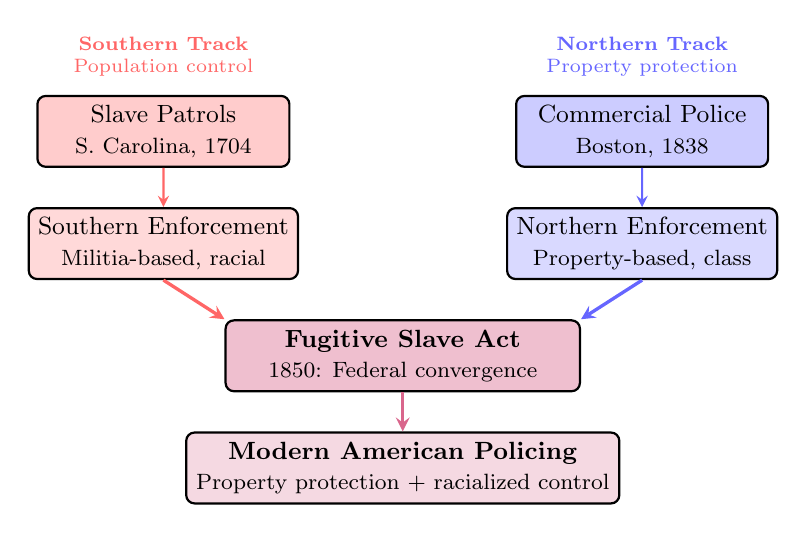
\begin{tikzpicture}[
      box/.style={draw, thick, rounded corners=3pt, minimum height=0.9cm, minimum width=3.2cm, align=center, font=\small},
      arr/.style={->, thick, >=stealth},
      scale=0.95
  ]
      % --- Southern branch ---
      \node[box, fill=red!20] (sp) at (-3.2,3) {Slave Patrols\\{\footnotesize S.\ Carolina, 1704}};
      \node[box, fill=red!15] (sc) at (-3.2,1.5) {Southern Enforcement\\{\footnotesize Militia-based, racial}};
      \draw[arr, red!60] (sp) -- (sc);

      % --- Northern branch ---
      \node[box, fill=blue!20] (np) at (3.2,3) {Commercial Police\\{\footnotesize Boston, 1838}};
      \node[box, fill=blue!15] (nc) at (3.2,1.5) {Northern Enforcement\\{\footnotesize Property-based, class}};
      \draw[arr, blue!60] (np) -- (nc);

      % --- Convergence point ---
      \node[box, fill=purple!25, minimum width=4.5cm, thick] (fsa) at (0,0) {\textbf{Fugitive Slave Act}\\{\footnotesize 1850: Federal convergence}};
      \draw[arr, red!60, very thick] (sc.south) -- (fsa.north west);
      \draw[arr, blue!60, very thick] (nc.south) -- (fsa.north east);

      % --- Modern policing ---
      \node[box, fill=purple!15, minimum width=5.5cm] (mod) at (0,-1.5) {\textbf{Modern American Policing}\\{\footnotesize Property protection + racialized control}};
      \draw[arr, purple!60, very thick] (fsa) -- (mod);

      % --- Labels ---
      \node[font=\scriptsize, red!60, align=center] at (-3.2,4) {\textbf{Southern Track}\\Population control};
      \node[font=\scriptsize, blue!60, align=center] at (3.2,4) {\textbf{Northern Track}\\Property protection};
  \end{tikzpicture}%
  }
  \caption{\textbf{The Dual Genealogy of American Policing.} Modern policing emerged from two distinct traditions: Southern slave patrols (1704) organized for racialized population control, and Northern commercial police (1838) organized for property protection. The Fugitive Slave Act (1850) federalized the slave patrol function, conscripting Northern police into Southern enforcement and fusing both mandates into a single institution.}
  \label{fig:policing_genealogy}
\end{figure}

\subsection{The Gendered Enforcement Gradient}

The application of the enforcement apparatus has historically been intersectional, targeting women of color with disproportionate brutality. Total executions of women were statistically rare compared to men. The racial disparity within those executions remains stark: between 1632 and 1962, 55\% of executed women were Black. This intersectional enforcement is detailed as part of the gendered axis analysis in Chapter~\ref{ch:gendered}.

\subsection{The Erasure of Extrajudicial Violence}

The documented figure of 356 executions is a vast underrepresentation of the true scale of state-sanctioned and state-tolerated violence against women, particularly Black women. During the antebellum period and the subsequent Jim Crow era, the murder of enslaved and free Black women often occurred outside the parameters of the formal legal system. Because enslaved individuals were legally categorized as property (Section 4.1), their deaths at the hands of enslavers were frequently treated as matters of property damage , with no homicide prosecution. The omission of thousands of unrecorded lynchings and localized executions underscores the inherent unreliability of historical data when assessing the true vulnerability of marginalized women to lethal state control.

\section{Introducing the Fourth Variable: The Enforcement Class ($F_{\text{enforce}}$)}

The slave patrol system reveals the structural necessity for a dedicated enforcement tier. The Elite ($E$) cannot personally actuate their extraction; doing so would expose them to the physical dangers of direct rule. The Buffer Class ($I_{\text{buffer}}$) provides ideological cover but lacks institutional authority. The system therefore required a specialized kinetic arm---recruited from the lower classes but compensated with unique privileges---to physically enforce the extraction algorithm.

\begin{definition}[The Enforcement Class]
\textbf{The Enforcement Class ($F_{\text{enforce}}$):} The kinetic arm of the algorithm ($F_{\text{enforce}} \subset I \cup O$). Comprising the military, domestic police forces, and carceral agents, they physically actuate the extraction. By design, $E$ recruits $F_{\text{enforce}}$ almost entirely from the lower classes. To ensure their compliance in inflicting brutality upon their own socioeconomic peers, $E$ compensates $F_{\text{enforce}}$ with a unique variable: \textbf{Qualified Immunity} ($QI$)---the judicial doctrine that shields state agents from civil liability for constitutional violations unless the victim can cite a prior case with nearly identical facts. The asymmetry of $QI$ is most starkly visible in the distribution of lethal autonomy. Under the Law Enforcement Officers Safety Act (LEOSA), active and retired members of $F_{\text{enforce}}$ are granted the statutory right to carry concealed firearms in all 50 states, superseding every state and local restriction. The Second Amendment thus operates on a strict gradient:
    \begin{equation}\label{eq:6.1-lethal-autonomy-gradient}
\text{Lethal Autonomy}(F_{\text{enforce}}) \gg \text{Lethal Autonomy}(I_{\text{buffer}}) \gg \text{Lethal Autonomy}(O) = 0
\end{equation}
    This gradient is the physical enforcement of the hierarchy. $F_{\text{enforce}}$ is granted superior armament precisely because they must be capable of overwhelming both the classes below them. Their status is strictly conditional; once a member of $F_{\text{enforce}}$ is no longer physically useful, their $QI$ is revoked, and they are discarded back into the Buffer Class or the Out-group.
\end{definition}

\noindent\textit{Illustrative instantiation (Tier~2, three-tier lethal autonomy gradient).} The three-tier gradient of eq.~\ref{eq:6.1-lethal-autonomy-gradient} is concretely anchored in statutory and historical law. At the top tier, the Law Enforcement Officers Safety Act (LEOSA, 18 U.S.C.~\S~926B) grants active and retired members of $F_{\text{enforce}}$ the right to carry concealed firearms in all 50 states, superseding every state and local restriction: $\text{LA}(F) \approx 1.0$. At the intermediate tier, Buffer Class ($I_{\text{buffer}}$) carry is governed by state-specific permit regimes with varying requirements---from shall-issue to may-issue to constitutional carry---placing $\text{LA}(I) \in [0.3, 0.7]$ depending on jurisdiction. At the base tier, $O_{\text{racialized}}$ faces systematic disarmament through a layered statutory architecture: the Mulford Act (1967) banned open carry explicitly in response to Black Panther monitoring patrols \cite{mulford1967}; the Sullivan Law (1911) established discretionary licensing designed to exclude immigrant and racialized populations from lethal autonomy \cite{sullivanlaw}; and felon-in-possession statutes (\usclink{apx:usc:18:922g}{18 U.S.C.~\S~922(g)}) apply asymmetrically through the racialized enforcement of the criminal pipeline above, effectively driving $\text{LA}(O) \to 0$. The gradient is therefore a structural invariant: each tier's lethal autonomy is calibrated to its position in the extraction hierarchy. \textbf{Confidence tier: Tier~2} --- statutory text is definitive; the ordinal gradient is confirmed by the legal record but not continuously measured; $\rho_\tau \in [0.5, 0.7]$.

\paragraph{Primary statutory text (LEOSA and civil-rights enforcement).}
The statutory asymmetry referenced above appears directly in federal law: \usclink{apx:usc:18:926b}{18 U.S.C.~\S~926B} (LEOSA) and the paired civil-rights statutes \usclink{apx:usc:18:241}{18 U.S.C.~\S~241} and \usclink{apx:usc:18:242}{18 U.S.C.~\S~242}.
\uscinline{usc_18_926b}
\uscinline{usc_18_241}
\uscinline{usc_18_242}

The structural role of $F_{\text{enforce}}$ is further revealed by a fact that most citizens find shocking when they first encounter it: \textbf{the police have no legal duty to protect you}. The Supreme Court has ruled---twice---that the Enforcement Class owes no constitutional obligation to protect individual citizens from harm, even when the danger is known and imminent. In \textit{DeShaney v.\ Winnebago County} (1989), the Court held that the state has no affirmative duty to protect individuals from private violence, even a child whose abuse the state had documented \cite{deshaney}. Chief Justice Rehnquist, for the majority, stated: ``[N]othing in the language of the Due Process Clause itself requires the State to protect the life, liberty, and property of its citizens against invasion by private actors.'' \textit{DeShaney}, 489 U.S.\ 189, 195 (1989). Justice Blackmun's dissent captured what the holding meant for the child: ``Poor Joshua! Victim of repeated attacks by an irresponsible, bullying, cowardly, and intemperate father, and abandoned by \textit{respondents} who placed him in a dangerous predicament and who knew or learned what was going on\ldots.''\footnote{Blackmun, J., dissenting, \textit{DeShaney v.\ Winnebago County Dep't of Social Servs.}, 489 U.S.\ 189, 213 (1989). Blackmun's dissent argued that once the state undertakes a ``special relationship'' with an individual---as the Winnebago DSS did with Joshua through documented visits and a removal that placed him back with his father---the Due Process Clause does impose an affirmative duty of protection. The majority's refusal to read a ``special relationship'' on the facts of \textit{DeShaney} produced the doctrinal baseline that subsequent cases like \textit{Castle Rock} extended to police enforcement duties.} In \textit{Town of Castle Rock v.\ Gonzales} (2005), the Court held that a woman had no enforceable right to police protection even when she held a restraining order against her estranged husband---who subsequently murdered their three children \cite{castlerock}. Justice Scalia, writing for the majority, held that a Colorado mandatory-arrest restraining order statute did not create a ``property'' interest in police enforcement enforceable under the Due Process Clause: ``A well-established tradition of police discretion has long coexisted with apparently mandatory arrest statutes.'' \textit{Castle Rock v.\ Gonzales}, 545 U.S.\ 748, 760 (2005) (Scalia, J.).\footnote{The framework reads the gendered specificity of \textit{Castle Rock} as structurally important. Jessica Gonzales held a statutory instrument---a restraining order issued by a court of law---that was explicitly designed to compel police enforcement. The Court's holding that even this instrument creates no enforceable right reveals that the $F_{\text{enforce}}$ discretion doctrine is not neutral: it operates against $O_{\text{gendered}}$ most severely precisely when $O_{\text{gendered}}$ is at greatest risk of lethal private violence. The system that disarms $O_{\text{gendered}}$ (Chapter~\ref{ch:gendered}) simultaneously removes the duty to protect $O_{\text{gendered}}$ from the private violence that weaponized disarmament enables. The two doctrines are not independent: they are the kinetic and enforcement sub-functions of the same extraction algorithm. \textit{DeShaney} removes the affirmative duty; \textit{Castle Rock} removes it even when a statutory instrument demands compliance. The combined holding produces a legal architecture in which the most vulnerable members of $O_{\text{gendered}}$ have no right to arms and no right to enforcement protection---simultaneously.}

Read these rulings through the framework and their logic becomes structurally transparent. $F_{\text{enforce}}$ does not exist to protect the population. It exists to \textit{enforce the extraction algorithm}. The legal doctrine confirms what the set-theoretic model predicts: the Enforcement Class serves $E$, not $O$ or $I_{\text{buffer}}$. The population is told that the police exist for their safety; the case law says otherwise. The system that disarms the population (Chapter~\ref{ch:kinetic}) simultaneously confirms, through its own judiciary, that the armed agents it deploys in their neighborhoods have no obligation to use that armament on their behalf. The asymmetry is total: $F_{\text{enforce}}$ is armed, immune, and \textit{not required to protect you}. You are disarmed, surveilled, and \textit{not entitled to their protection}. The system is operating exactly as designed.

The foundational inequality now extends to four tiers:
\begin{equation}\label{eq:6.2-four-tier-benefit-ordering}
\text{Benefit}(E) \gg \text{Benefit}(F_{\text{enforce}}) > \text{Benefit}(I_{\text{buffer}}) > \text{Benefit}(O_{\text{racialized}})
\end{equation}
where $\text{Benefit}(F_{\text{enforce}})$ consists of Qualified Immunity ($QI$), enhanced lethal autonomy, and zero accountability to the populations they nominally serve.

\subsection*{Case Study: Police Killings and the Enforcement Benefit Hierarchy}
\label{cs:police_killings}

\paragraph{Setup.}
Equation~\ref{eq:6.2-four-tier-benefit-ordering} specifies a strict benefit hierarchy across the four tiers of the extraction system. For the enforcement layer ($F_{\text{enforce}}$), the framework makes a testable prediction about the \textit{distribution} of enforcement lethality: if the purpose of $F_{\text{enforce}}$ is to protect $E$'s extraction interests, leaving the population at large unprotected, then enforcement lethality should be concentrated at the bottom of the hierarchy---against $O_{\text{racialized}}$---and approach zero at the top. Per-capita police killing rates by racial group provide a direct, measurable operationalization of this prediction.

\paragraph{Data sources.}
Per-capita police killing data are drawn from the Mapping Police Violence dataset \cite{mapping_police_violence}, which maintains the most comprehensive public database of police killings in the United States. Population denominators are from U.S. Census Bureau American Community Survey one-year estimates for 2013--2022 and Census Bureau population estimates for 2023--2024. Data cover 2013--2024 with breakdowns by race: Black, White, Hispanic, Native American, and Asian. Curated data are archived at \texttt{Paper/data/eq27\_police\_killings.csv}; computational results are reproducible via \texttt{Paper/scripts/eq27\_police\_killings.ipynb}.

\paragraph{Operationalization.}
The benefit hierarchy from Equation~\ref{eq:6.2-four-tier-benefit-ordering} is operationalized against per-capita killing rates as follows. $O_{\text{racialized}}$ is represented by Black and Native American populations, which the framework predicts to bear the highest enforcement lethality. $I_{\text{buffer}}$ is represented by Hispanic and White (non-elite) populations, which the framework predicts to bear intermediate rates. $F_{\text{enforce}}$ and $E$ are predicted to bear near-zero lethality from their own enforcement apparatus by construction.

\paragraph{Numerical computation.}
Averaging across the full 2013--2024 period, the notebook yields the following per-capita killing rates (per million population): Black, 7.00; Native American, 6.55; Hispanic, 2.89; White, 2.33; Asian, 0.91. The Black-to-White per-capita ratio averages 3.01 across the period. The Native American-to-White ratio averages 2.81. The $O_{\text{racialized}}$ tier average (Black and Native American combined) is 6.78 per million; the $I_{\text{buffer}}$ tier average (Hispanic and White combined) is 2.61 per million---a ratio of approximately 2.6:1. At peak years (2015--2016), the Black per-capita rate exceeded 8 per million, while the White rate remained below 2.9 per million.

\begin{figure}[htbp]
  \centering
  
\includegraphics[width=\textwidth]{figures/eq27_police_killings.png}
  \caption{Police killing rates by racial group, 2013--2024 (per million population per year, Mapping Police Violence data). Groups are ordered by tier position: $O_{\text{racialized}}$ (Black, Native American) sustain the highest rates; $I_{\text{buffer}}$ groups (Hispanic, White, Asian lower sub-position) cluster at intermediate rates. The monotonic hierarchy across all five groups confirms the tier-benefit ordering of eq.~\ref{eq:6.2-four-tier-benefit-ordering}.}
  \label{fig:eq27_police}
\end{figure}

\paragraph{Comparison to prediction.}
Equation~\ref{eq:6.2-four-tier-benefit-ordering} predicts Benefit$(E) \gg$ Benefit$(F_{\text{enforce}}) >$ Benefit$(I_{\text{buffer}}) >$ Benefit$(O_{\text{racialized}})$. Mapping this onto enforcement lethality (where lower benefit = higher lethality exposure), the predicted ordering is: $O_{\text{racialized}}$ killed at the highest rate, $I_{\text{buffer}}$ at intermediate rates, $F_{\text{enforce}}$ and $E$ at near-zero. The data confirm the predicted ordering without exception: the Black per-capita rate (7.00) exceeds the Hispanic rate (2.89), which exceeds the White rate (2.33), which exceeds the Asian rate (0.91)---a monotonic hierarchy consistent with the framework's tier structure. The 3:1 Black-to-White ratio is stable across an 11-year period spanning multiple administrations, multiple policy changes, and the social disruption of 2020.

\paragraph{Falsification criteria.}
This equation would be falsified if per-capita police killing rates were uniform across racial groups---i.e., if enforcement lethality showed no systematic relationship to the predicted tier hierarchy. It would also be falsified if the rate for $I_{\text{buffer}}$ exceeded the rate for $O_{\text{racialized}}$ across a sustained period, inverting the predicted hierarchy. The 2013--2024 data show neither condition. The Black-to-White gap has narrowed slightly from peak years (2015--2016) but has not closed, and in no year does the White per-capita rate approach the Black rate. The hierarchy is stable across the full measurement window.

\paragraph{Confidence tier.}
\textbf{Tier~1.} Eleven-year continuous dataset from a purpose-built tracking database; the racial hierarchy in per-capita killing rates is statistically stable across the full period; the ordering is consistent with the tier predictions of eq.~\ref{eq:6.2-four-tier-benefit-ordering} without requiring parameter calibration.

\subsection{The Gang Morphology of the Enforcement Class}

The claim that $F_{\text{enforce}}$ operates as a structurally distinct caste---loyal to itself before the public it nominally serves---is empirically observable in the Enforcement Class's adoption of its own iconography, its documented formation of literal internal gangs, and its violent hostility toward any civilian who reminds them of their subordinate constitutional role.

\paragraph{Federal ``criminal street gang'' definition (contrast).}
For contrast with informal ``gang'' iconography inside enforcement institutions, Congress separately defines a \emph{federal} criminal street gang in \usclink{apx:usc:18:521}{18 U.S.C.~\S~521}:
\uscinline{usc_18_521}

\textbf{The Thin Blue Line Flag: A Gang Identifier}

Sociologically, gangs are defined in part by shared symbols, group loyalty superseding institutional norms, and hostility toward outsiders. The ``Thin Blue Line'' flag---a black-and-white American flag bisected by a single blue stripe---meets every criterion. It emerged as a mass-adopted identity marker explicitly in opposition to the Black Lives Matter movement (post-2014), functioning as an \textit{oppositional identity symbol}: its wearers define themselves \textit{against} accountability. The flag signals unconditional in-group loyalty, and social penalties attach to members of $F_{\text{enforce}}$ who refuse to display it. Some departments---including San Francisco---have banned the flag on duty, recognizing that it had become a politically charged tribal marker \cite{skolnick}.

The flag's ideological function is revealing: $F_{\text{enforce}}$ has replaced the national flag---the symbol of the constitutional republic they swore to serve---with their own. The image declares a parallel sovereignty. The Enforcement Class signals, in plain iconography, that their primary allegiance is to the blue caste, not to the public.

\textbf{Literal Gang Formation: The LASD Proof}

The Los Angeles County Sheriff's Department provides the most extensively documented case of literal gang formation within the Enforcement Class. Over five decades, named deputy gangs---the \textbf{Lynwood Vikings}, the \textbf{Banditos}, the \textbf{Executioners}, the \textbf{Reapers}, and others---have operated within LASD stations with matching tattoos, initiation rituals, and internal hierarchies indistinguishable from street gangs.

The Lynwood Vikings were found by a federal jury to be a ``neo-Nazi, white supremacist gang'' within the department (\textit{Thomas v. County of Los Angeles}, 1991). The Banditos, based at the East Los Angeles Station, allegedly demanded ``taxes''---a portion of other deputies' overtime pay---controlled work assignments, and physically assaulted deputies who refused to comply. The Executioners, at the Compton Station, allegedly required deputy-involved shootings as a prerequisite for full membership, with members celebrating kills \cite{lacoversight}.

In 2022, the Los Angeles County Civilian Oversight Commission confirmed that deputy gangs had existed within the LASD for over fifty years and that the department had structurally failed to eradicate them. California was forced to pass Assembly Bill 958 (2021), requiring law enforcement agencies to maintain policies against gang participation---the state legislature effectively acknowledging that the Enforcement Class had to be \textit{legally prohibited} from operating as organized criminal enterprises.

The NYPD exhibits analogous patterns without the formal tattoo structure. The Mollen Commission (1994) documented organized crews of officers---particularly in the 30th Precinct in Harlem, known as the ``Dirty Thirty''---who engaged in systematic drug trafficking, robbery, and perjury, enforcing silence through threats and retaliation against whistleblowers.

\textbf{The First Amendment Audit Proof: Hostility Toward Public Accountability}

Perhaps the most accessible, real-time evidence of the Enforcement Class's caste psychology is provided by the First Amendment auditing community. Independent journalists and citizen auditors---documented extensively by channels such as \textit{Long Island Audit} (Sean-Paul Reyes), \textit{Delete Lawz} (Chille DeCastro), and the analytical channel \textit{Audit the Audit}---exercise the constitutionally protected right to film in public spaces: post offices, police station lobbies, town hall meetings, and public sidewalks.

Federal case law is unambiguous: filming government officials performing their duties in public spaces is protected by the First Amendment (\textit{Glik v. Cunniffe}, 655 F.3d 78, 1st Cir. 2011; \textit{Turner v. Driver}, 848 F.3d 678, 5th Cir. 2017). Across thousands of documented encounters, the single statement most likely to escalate a lawful interaction into a detention or arrest is some variation of: ``You work for me,'' ``You're a public servant,'' or ``This is a public building paid for with my taxes.'' Officers respond to these \textit{factually accurate, constitutionally protected statements} with visible rage, unlawful orders to stop filming, demands for identification without reasonable suspicion, and retaliatory arrest.

This pattern is diagnostic. The Enforcement Class's violent allergic reaction to being reminded of its public-servant status reveals the depth of the caste inversion. $F_{\text{enforce}}$ experiences itself as sovereign over the citizenry. The auditing community has inadvertently constructed the largest decentralized empirical dataset proving that the Enforcement Class operates with a self-conception fundamentally incompatible with democratic governance. They are an occupying force that occasionally tolerates the public.

\section{The Asymmetric Distribution of Lethal Autonomy: The Second Amendment and the Haitian Proof}

Within the framework of systemic oppression, the United States Constitution’s Second Amendment provides the most stark example of a system functioning exactly as programmed, despite its ideological justification (Component 3). Nominally presented as a universal safeguard against tyranny, the Second Amendment was engineered by the Elite ($E_{US}$) with a specific, exclusionary "bug." Its functional purpose was the asymmetric distribution of lethal autonomy.

Mathematically, the right to bear arms was granted to the Buffer Class ($I \setminus E$) specifically to empower the "well-regulated militias"—which, in the Southern operational zone, were explicitly the slave patrols. Lethal autonomy was distributed to the In-group for the sole purpose of enforcing the physical boundaries of the Out-group ($O$).

\subsection{The Constitutional Dialectic: Natural Rights and Restricted Recognition}
\label{sec:constitutional_dialectic}

The framework's critique of the Second Amendment requires an explicit methodological concession absent from the surrounding literature. The left-coded and right-coded interpretations of the American constitutional order are \textit{both structurally correct}. Each reading captures one structural variable; the true interpretation compiles both.

\textbf{The originalist reading (ontology of the right).} The originalist / right-coded interpretation correctly identifies that the Second Amendment recognizes a pre-existing right to keep and bear arms. The Framers took this right to pre-exist the state itself---grounded in the Lockean natural-rights tradition that the Declaration of Independence had already encoded as self-evident (``unalienable Rights''), and in the explicit constitutional mandate that a tyrannical government can and must be overthrown. On this reading, the right is pre-political. It belongs to every human being by virtue of being a human being. The state's only constitutional role is the recognition and non-infringement of what was already there. The originalists are telling the truth about the \textit{ontology} of the right.

\textbf{The expansionist reading (scope of recognition).} The left-coded / expansionist interpretation correctly identifies that the operational scope of that recognition was engineered to be narrow. The system \textit{recognized} these pre-existing natural rights exclusively for white, propertied, male members of the In-group. The same text that the originalist reads as universal was compiled, in practice, for a demographically bounded class. The Constitution's stated spirit---``We the People,'' ``all men,'' ``unalienable''---pointed unmistakably toward universal application. The Framers' operational code restricted recognition to themselves. The expansionists are telling the truth about the \textit{scope} of recognition.

\textbf{The synthesis.} The framework resolves the apparent contradiction by separating these two variables. Let $R_{\text{natural}}(x)$ denote the pre-political natural right to kinetic self-defense possessed by every human $x$, and let $S_{\text{recognition}}(x, t)$ denote whether the state formally recognizes that right for individual $x$ at time $t$. The Framers' constitutional architecture is the assertion:
\begin{equation}\label{eq:const_dialectic}
\forall x \in \text{Humans}: R_{\text{natural}}(x) = \text{TRUE} \quad \land \quad S_{\text{recognition}}(x, 1791) = \mathbf{1}[x \in I_{\text{propertied, white, male}}].
\end{equation}

The originalist reads the first conjunct and concludes the right is universal. The expansionist reads the second conjunct and concludes the right is a class privilege. \textit{Both are correct}. The paper's entire argument is that liberation under this constitutional order requires forcing the second conjunct to converge on the first. The domain of $S_{\text{recognition}}$ must be expanded until it equals the domain of $R_{\text{natural}}$. That is the operation the Out-group has been forcing, kinetically and legally, for two and a half centuries.

\textbf{The Framers knew exactly what they were doing.} The dialectic above is a description of what the Framers consciously engineered. These men were the architects of a \textit{deliberately genocidal slave state}---a political economy built on chattel slavery, continental-scale Indigenous dispossession, and the near-total disarmament of the populations they were extracting from. The design was intentional.

This matters because it forecloses the sentimental reading in which the Second Amendment's exclusionary compilation was a regrettable oversight that history has been slowly correcting. If the Framers designed a system whose survival required asymmetric lethal capacity ($L_E \gg L_O$), they understood the Second Amendment's structural function with engineering precision. A man who builds a slave state arms the slaves deliberately. He articulates, in the Declaration, a philosophical justification for armed overthrow of tyranny that would---if universalized---terminate his own operation. He writes those words \textit{while knowing} they would terminate his operation if the recognition domain were ever expanded to include the people he was enslaving. The Framers' genius and the Framers' horror are the same fact: they understood the Second Amendment's meaning completely, and they installed it anyway, with the recognition domain restricted to themselves.

This is the only reading that makes their subsequent terror of Haiti computationally coherent. If the Framers had believed, as the sentimentalist reconstruction claims, that the Second Amendment was a narrowly civic provision about militia regulation, the Haitian Revolution would have registered as a foreign disturbance of marginal structural relevance. It did not. It produced an immediate, multi-decade continental panic (documented in \S~\ref{sec:haitian_instantiation} and \S~\ref{sec:haitian_contagion}), culminating in the Louisiana Purchase, the Negro Seamen Acts, the quarantining of Haitian diplomatic recognition, and the \textit{Dred Scott} security patch of 1857. The American Elite's response was the correct magnitude of response for men who knew exactly what they had designed. They had written the anti-tyranny protocol. They had seen the Haitians compile and execute it. They understood, in real time, that their own constitutional architecture, executed without the racist parameters installed by the colonial Elite, would destroy them. Their panic registered recognition.

The remainder of this section formalizes that recognition.

\subsection{The Haitian Instantiation: Executing the "Pure" Code}
\label{sec:haitian_instantiation}
The ultimate proof of this structural hypocrisy occurred contemporaneously in Saint-Domingue. The Haitian Revolution (1791-1804) was essentially a perfect, real-world instantiation of the core philosophy of the Second Amendment. An armed, subjugated populace recognized a tyrannical, extractive government and utilized lethal force to violently dismantle it.

The global Elite ($E_{\text{global}}$) classified Out-group execution of the protocol as a catastrophic system error. An In-group execution would have been recognized as a triumph of liberty. The Haitian Revolution was the Second Amendment compiled and run without the racist parameters installed by the colonial Elite. It demonstrated that if the Out-group achieves lethal parity, the Predatory Min-Max Function completely collapses.

\subsection{The Christiana Proof: The Anti-Tyranny Protocol Executes on American Soil (1851)}

The Haitian scenario replicated domestically. It happened in Pennsylvania.

On September 11, 1851, Maryland slaveholder Edward Gorsuch arrived at the farmhouse of \textbf{William Parker}---a formerly enslaved man living free in Christiana, Pennsylvania---accompanied by a deputy U.S.\ Marshal, his son, and several slave catchers. They came to recapture four men who had escaped from Gorsuch's plantation, armed with the full legal authority of the \textbf{Fugitive Slave Act of 1850}, which compelled citizens of free states to assist in the capture of escaped enslaved people and denied the accused any right to trial by jury \cite{christiana_history, christiana_zinn}.

Parker refused to comply. His wife Eliza sounded a horn from the upper window, alerting the surrounding community. Within the hour, dozens of free Black residents---joined by several white Quaker neighbors---surrounded Gorsuch's party with firearms, corn cutters, and clubs. When Gorsuch refused to withdraw, a firefight erupted. Edward Gorsuch was killed. His son was badly wounded. The deputy U.S.\ Marshal fled. The four freedom seekers escaped to Canada through the Underground Railroad. Parker followed them.

The federal government's response revealed the system's deepest fear. President Fillmore dispatched a company of U.S.\ Marines and a posse of federal marshals to Christiana and charged \textbf{41 defendants}---Black and white---with \textbf{treason} against the United States. \textit{Treason}---the most severe charge in the federal code, carrying the death penalty. The government argued that armed resistance to the Fugitive Slave Act constituted ``levying war'' against the nation \cite{christiana_history}.

The treason trial of Castner Hanway---a white Quaker miller who had merely refused to assist the slave catchers---became a national spectacle. His defense was led by Thaddeus Stevens, the abolitionist congressman. The jury acquitted Hanway in \textbf{fifteen minutes}. The government quietly dropped all remaining charges.

Read Christiana through the framework. The Out-group compiled the anti-tyranny protocol---the same code Haiti had executed---on domestic soil. A free Black community armed itself, organized collective defense, and killed a slaveholder who arrived backed by federal law. The system's response was the charge of \textit{treason}---the legal instrument reserved for existential threats to the state. The message was structural: when $O_{\text{racialized}}$ exercises the kinetic guarantee against $E$’s enforcement apparatus, the system does not process it as self-defense. It processes it as war.

Six years later, Chief Justice Taney would articulate the precise fear that Christiana had instantiated.

\subsection{Weaponizing Disarmament: The Dred Scott Proof and the Elite’s Security Patch}
Observing the success of the Haitian model---and its domestic replication at Christiana---the American Elite panicked. If the Out-group ($O$) internalized the true logic of the Second Amendment, the domestic extraction engine would be destroyed. The systemic necessity to disarm the Out-group was explicitly articulated by the Elite's highest judicial authority in the 1857 \textit{Dred Scott v. Sandford} decision.

In his majority opinion, Chief Justice Roger Taney ruled that Black Americans could not be citizens. To justify this, he revealed the core algorithmic fear of the Elite: if Black people were granted citizenship, it would entitle them to the full privileges of the In-group, which would give them the right ``to keep and carry arms wherever they went''---``inevitably producing discontent and insubordination among them, and endangering the peace and safety of the State.'' \textit{Dred Scott v.\ Sandford}, 60 U.S.\ 393, 416--417 (1857) \cite{dredscott}.

Taney’s opinion acts as a formal, legal admission of the system's design. The Elite ($E_{US}$) understood that an armed Out-group was an existential threat to capital. Consequently, they weaponized the law to aggressively disarm Black Americans.

This initiated an unbroken historical algorithm of racialized disarmament. From the antebellum Black Codes that made it a severe crime for any Black person (free or enslaved) to own a firearm, to the post-Civil War disarmament sweeps by white terror groups, and culminating in modern gun control legislation (such as the Mulford Act of 1967, passed explicitly to disarm the Black Panthers), the system has constantly generated new proxy variables ($P$) to restrict the Out-group's access to self-defense.

Within this framework, the Second Amendment operates on a strict dual-track algorithm:
\begin{itemize}
    \item When the Buffer Class ($I \setminus E$) arms itself, the system recognizes it as a constitutionally protected expression of liberty.
    \item When the Out-group ($O$) arms itself, the system triggers an immediate threat response, reclassifying the behavior as "criminality" or "rebellion," thereby legally authorizing the deployment of the policing enforcement mechanism.
\end{itemize}

The history of American gun control is, therefore, a continuously updated security patch engineered by the Elite to prevent the domestic Out-group from ever replicating the Haitian instantiation of true autonomy.

\subsection{The Physical Guarantee: The Second Amendment as Collateral}

Traditional analyses of the Second Amendment often limit its utility to either the preservation of a national militia or the localized enforcement of slave patrols. Within the framework of the Predatory Min-Max Function, the asymmetrical distribution of lethal autonomy served a much deeper structural purpose: it was the Elite's ($E$) physical collateral to underwrite the 1705 contract.

When the Elite partitioned the poor and created the Buffer Class ($I_{\text{buffer}}$), they required absolute assurance that this new working-class In-group would permanently side with Elite interests over cross-class solidarity with the Out-group ($O$). The psychological wage ($\psi$) of ``Whiteness'' was insufficient on its own; $I_{\text{buffer}}$ required a tangible guarantee that they would never be subjected to the extraction kernel.

The Second Amendment, particularly when philosophically paired with the Declaration of Independence's mandate to overthrow tyrannical governments, functioned as this guarantee. By legally distributing lethal parity to the Buffer Class, the Elite formalized a transactional promise: ``We guarantee you will never become slaves, and to prove it, we are handing you the physical tools to violently destroy us if we ever attempt to treat you as the Out-group.'' It was the ultimate systemic pacifier, convincing $I_{\text{buffer}}$ that they held the ultimate veto over Elite power, effectively ensuring their complicity in the subjugation of $O$.

The guarantee derived its force from proximity. The Buffer Class's alignment with the Second Amendment was underwritten by direct, daily knowledge of exactly what they were being guaranteed against. The plantation was visible. The horror was documented, witnessed, and understood---across the fence line, in the fields, in the quarters. When the 1705 contract promised $I_{\text{buffer}}$ that they would never be subjected to the extraction kernel, it pointed at something specific---something $I_{\text{buffer}}$ could see from the road. The consequence is that the Buffer Class's constitutional alignment was a terror-anchored commitment: they would protect the system that produced those horrors because the system's continued operation was proof that those horrors would bypass them. Any threat to the system was experienced as a threat to that guarantee. This explains the intensity that the framework's kinetic analysis must account for: a population defending a witnessed boundary between themselves and what they knew was on the other side of it.

The Necessary Condition Theorem (Section~\ref{sec:necessary_condition}) reveals the structural inversion beneath this arrangement. The Second Amendment is framed as $E$ protecting $I_{\text{buffer}}$: the Elite gifting the Buffer Class the tools to resist tyranny. The demographic mathematics of the antebellum system invert this framing. The Elite could not maintain $M(t) < \tau$ without $K_B$. The weapons were a \textit{payment} to the Buffer Class for the service the Elite desperately required: the daily enforcement of a system that would have collapsed the moment the numerically superior, armed buffer class turned those weapons toward liberation and away from suppression. The Second Amendment was the Elite purchasing the necessary condition of their own survival---and constructing a narrative in which the Buffer Class believed the transaction ran the other way.

\subsection{The General Strike of the Enslaved: Du Bois's Proof of Out-Group Kinetic Agency}
\label{sec:general_strike_sub}

The preceding analysis has located the Civil War as the kinetic rupture that forced the 13th Amendment. The standard historiography frames this rupture as a gift from above: Lincoln's executive intervention ending slavery. W.E.B.\ Du Bois's \textit{Black Reconstruction in America} is the definitive refutation of that framing \cite{dubois}.

Du Bois's fourth chapter, ``The General Strike,'' documents what the conventional narrative systematically erases: beginning in 1861 and accelerating through 1864, approximately 500,000 enslaved people exercised the only kinetic option available to them and walked off the plantations. They did not wait for emancipation. They emancipated themselves---streaming into Union lines, overwhelming contraband camps, supplying military intelligence that no Northern spy network could replicate, and withdrawing the labor force that was the Confederacy's logistical foundation. Du Bois calculated that this mass self-emancipation constituted, in structural terms, a \textbf{general strike}: the coordinated withdrawal of labor by an entire class, executed without formal organization, against a system that had made organization criminally impossible.

The strategic consequences were irreversible. The Confederacy's war machine depended on enslaved labor for agriculture, fortification-building, supply transport, and the full logistics of fielding an army. As the general strike scaled, Confederate productive capacity collapsed faster than Union military operations could have achieved. Lincoln's Emancipation Proclamation (1863)---documented in the Concession Theorem (Section~\ref{sec:concession_theorem}) as a military strategy---was the Union government's institutional recognition of a fact $O_{\text{racialized}}$ had already created on the ground. The Out-group broke the algorithm's grip unilaterally, and the algorithm's legal interface was subsequently rewritten to accommodate that fact.

The framework must integrate this proof explicitly. The Haitian Theorem (Section~\ref{sec:haitian_theorem}) establishes kinetic action as the only historically validated liberation mechanism at the colonial scale. The general strike establishes that the same mechanism operated domestically---that the kinetic capacity of $O_{\text{racialized}}$, exercised collectively and without waiting for elite authorization, is what forced the system update. The 13th Amendment, which follows immediately below, was the Elite's recompilation around the Out-group's successful kernel breach. Understanding the sequence in this order---kinetic Out-group action first, legal patch second---is essential to the framework's predictive architecture.

\begin{figure}[htbp]
\centering
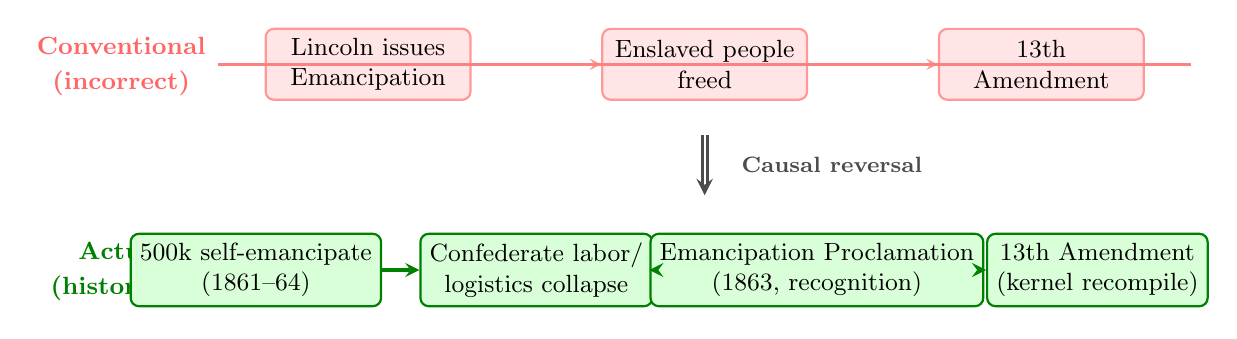
\begin{tikzpicture}[
    box/.style={draw, thick, rounded corners=3pt, minimum height=0.9cm, minimum width=2.6cm, align=center, font=\small},
    arr/.style={->, thick, >=stealth},
    scale=0.95
]
    % --- Conventional (incorrect) row ---
    \node[font=\small\bfseries, red!60] at (-5.8,1.5) {Conventional};
    \node[font=\small\bfseries, red!60] at (-5.8,1.0) {(incorrect)};
    \node[box, fill=red!10, draw=red!40] (a1) at (-2.5,1.25) {Lincoln issues\\Emancipation};
    \node[box, fill=red!10, draw=red!40] (a2) at (2,1.25) {Enslaved people\\freed};
    \node[box, fill=red!10, draw=red!40] (a3) at (6.5,1.25) {13th\\Amendment};
    \draw[arr, red!40] (a1) -- (a2);
    \draw[arr, red!40] (a2) -- (a3);
    % Strike-through
    \draw[very thick, red!50] (-4.5,1.25) -- (8.5,1.25);

    % --- Reversal arrow ---
    \draw[arr, very thick, black!70, double] (2,0.3) -- (2,-0.5);
    \node[font=\footnotesize\bfseries, black!70] at (3.7,-0.1) {Causal reversal};

    % --- Correct row ---
    \node[font=\small\bfseries, green!50!black] at (-5.8,-1.25) {Actual};
    \node[font=\small\bfseries, green!50!black] at (-5.8,-1.75) {(historical)};
    \node[box, fill=green!15, draw=green!50!black] (b1) at (-4,-1.5) {500k self-emancipate\\(1861--64)};
    \node[box, fill=green!15, draw=green!50!black] (b2) at (-0.25,-1.5) {Confederate labor/\\logistics collapse};
    \node[box, fill=green!15, draw=green!50!black] (b3) at (3.5,-1.5) {Emancipation Proclamation\\(1863, recognition)};
    \node[box, fill=green!15, draw=green!50!black] (b4) at (7.25,-1.5) {13th Amendment\\(kernel recompile)};
    \draw[arr, green!50!black, very thick] (b1) -- (b2);
    \draw[arr, green!50!black, very thick] (b2) -- (b3);
    \draw[arr, green!50!black, very thick] (b3) -- (b4);
\end{tikzpicture}
\caption{\textbf{The General Strike: Causal Timeline Reversal.} The conventional framing (top) assumes legal decree produced social change. The historical evidence (bottom) reveals that out-group kinetic action (the General Strike) collapsed the existing system's logistics, forcing the legal apparatus to recognize the new reality through the Emancipation Proclamation and the subsequent 13th Amendment patch.}
\label{fig:general_strike_causal}
\end{figure}

\section{The System Kernel: The 13th Amendment Loophole (1865)}
Following the Civil War, the system required a new legal kernel. The \textbf{13th Amendment} converted slavery from a static identity to a conditional state via the exception clause: \textit{``except as a punishment for crime''} \cite{alexander, blackmon, thirteenth}.

\begin{equation}\label{eq:6.3-thirteenth-amendment-exception}
\text{If} \quad \text{Status}(x) = \text{Criminal}(C) \quad \rightarrow \quad \text{Status}(x) \in S \text{ (Slave)}
\end{equation}

This\footnote{This equation is classified as Tier~3 (ordinal/structural); the conditional re-enslavement via criminal conviction is a structural claim validated by the convict leasing system documented in Blackmon (2008) \cite{blackmon} and the mass incarceration data in Alexander (2010) \cite{alexander}. See the Empirical Methodology chapter (p.~\pageref{ch:empirical_methodology}) and Appendix~\ref{app:empirical_index}.} ensured that slavery remained a constitutionally protected state, accessible to the Elite as long as they could map the target population to the variable of Criminality ($C$).

\paragraph{The statutory contradiction.}
Federal law nominally criminalizes involuntary servitude under \usclink{apx:usc:18:1581}{18 U.S.C.~\S~1581} (Peonage) and \usclink{apx:usc:18:1589}{18 U.S.C.~\S~1589} (Forced labor). The 13th Amendment's exception clause simultaneously permits it for the incarcerated:
\uscinline{usc_18_1581}
\uscinline{usc_18_1589}

\subsection{The Interface Swap: Why ``Progress'' Escalates Brutality}

When observing the historical timeline, the transition from chattel slavery to convict leasing following the 13th Amendment is conventionally framed as moral progress. Under the mathematical framework of systemic extraction, we must evaluate the reality on the ground: an interface swap often removes the few physical constraints the Elite previously had, thereby escalating the brutality.

Under chattel slavery, the Elite ($E$) had a direct financial investment in the biological survival of the enslaved worker. Destroying the asset entirely would have represented a loss of capital even under absolute extraction. This created a dark, but functional, biological ceiling on the extraction rate.

When the system updated its interface to convict leasing---utilizing the constitutional loophole to transition the Out-group into carceral slavery---this capital constraint was permanently removed. The Elite no longer owned the bodies; they simply leased the labor from the State. Because the carceral system, fed by the newly minted Black Codes, provided an infinite, subsidized stream of replacement bodies, the Elite had zero financial incentive to keep the laborers alive. The optimal economic strategy shifted to extracting maximum labor in minimum time, even if it resulted in the death of the worker. Consequently, mortality rates in convict leasing camps frequently exceeded those of chattel slavery. The ``upgrade'' to the system did not mitigate the extraction kernel; it optimized the brutality by socializing the cost of replacing the human capital.

This finding confirms the escalation thesis. Economic historians document measurably higher output-per-worker in targeted sectors---Alabama coal mines, railroad construction, turpentine and phosphate extraction---under convict leasing than under antebellum chattel slavery. Daily quotas increased; absenteeism fell; piece-rate throughput accelerated. These efficiency gains are the \textit{mechanism} of the interface swap's escalatory effect. Elevated mortality and elevated throughput are two simultaneous measurements of the same removed constraint. When replacement cost is driven to zero by state subsidy ($\text{Cost}_{\text{replacement}} \to 0$), the lessee's rational strategy is to extract the maximum possible output per unit time until the biological asset is consumed---and then draw the next body from the pipeline. The result is that $E$ records higher throughput \textit{and} $O$ records higher mortality because the same removed constraint produces both. Both are products of the same optimization: $\Delta_{\max}$ preserved and expanded by treating the Out-group as a fully disposable input. Any analysis that cites productivity gains as a qualification of the brutality claim has measured the Elite's ledger and forgotten to measure the cost at which it was balanced.

\subsection{The Culling Variable: Consumptive Extraction and Demographic Control}

To fully understand the brutality of the post-1865 algorithmic update, we must evaluate convict leasing as a deliberate demographic culling of the racialized Out-group ($O_{\text{racialized}}$).

Under the pre-1865 interface (chattel slavery), the Out-group was legally classified as capital. Consequently, the Elite ($E$) possessed a direct financial imperative to manage the mortality rate ($M$) of the enslaved population. The conditions were horrific; destroying the asset entirely would have represented a loss of wealth on the Elite's ledger. The algorithm required extraction to remain just below the threshold of biological collapse.

The 13th Amendment Loophole effectively externalized the cost of mortality. By shifting the Out-group from ``owned capital'' to ``leased state property,'' the Elite achieved a terrifying economic freedom: they no longer bore the replacement cost of the human beings they worked to death. Because the newly implemented Black Codes---the $P_{\text{criminal}}$ proxy---guaranteed a continuous, subsidized pipeline of replacement bodies, the functional constraint on mortality was permanently deleted from the source code.

Within the Tri-Modal Enclosure Model (Equation~\ref{eq:1.1-enclosure-score}), the Black Codes and the 13th Amendment exception clause constituted an \textbf{enclosure repair} executed after Abolition had briefly opened all three channels. Emancipation threatened to lower $e_1$ (communal capacity) by permitting freedpeople to build schools, churches, and mutual-aid societies; to lower $e_2$ (geographic/economic mobility) by removing the legal barriers to movement and contract; and to lower $e_3$ (psychological/epistemic autonomy) by allowing Black civic participation and the very act of self-naming as citizens. The Black Codes reversed each of these gains: vagrancy laws and curfews tightened $e_2$; the destruction of Reconstruction-era institutions (Freedmen's Bureau schools, Black banks, elected Black officials) tightened $e_1$; and the reimposition of white judicial supremacy tightened $e_3$ by teaching the population that even formal freedom remained contingent on white consent. The enclosure score \(\mathcal{S}_{\text{enc}}(O_{\text{racialized}})\), which had momentarily dropped after 1865, was driven back toward $1.0$ within a single decade.

Mathematically, the extraction kernel evolved into a \textbf{Consumptive Extraction Function}. The optimal economic strategy for the lessee was to extract maximum caloric and physical labor in the absolute minimum time, fully consuming the biological asset until death, and then simply leasing a replacement.

This hyper-lethal environment---where annual mortality rates in certain mining and railroad camps routinely exceeded 30 to 40 percent---was a dual-purpose optimization by the Elite:

\begin{enumerate}
    \item \textbf{Maximum Profit:} It generated unprecedented profit margins by reducing overhead (food, medical care, shelter) to near-zero.

    \item \textbf{Demographic Culling:} It solved the nascent threat of the Demographic Paradox (Section~6.6). The physical elimination of thousands of working-age men from $O_{\text{racialized}}$ functioned as a brutal population control mechanism. By literally working a massive segment of the Out-group to death, the system neutralized the political and demographic threat of a newly emancipated populace before they could achieve operational solidarity or electoral power.
\end{enumerate}

Convict leasing, therefore, constituted an algorithmic escalation. It transformed the extraction engine into a meat grinder, utilizing state-sponsored criminalization to legally cull a population that the Elite needed to control without directly owning.

\subsection{The Transition Function: Forced Industrialization of the South}

The preceding subsections document convict leasing as a labor extraction system and a demographic culling mechanism. The framework also identifies its \textit{third} structural function---one that explains why the system constituted a necessary precondition for the South's entry into the industrial economy.

Prior to 1865, the Southern economy was overwhelmingly agrarian, built on and backed by enslaved human capital. The Northern economy had already industrialized. The 13th Amendment \textit{annihilated the economic model of an entire region}. The South's capital base---which had been denominated in human bodies, cotton futures, and plantation acreage---required a total structural transition to integrate into the industrial economy that the North had been building for decades. Railroads had to be laid. Mines had to be opened. Levees, roads, and turpentine camps had to be constructed. The infrastructure of industrialization required precisely the kind of massive, expendable, unskilled labor force that the plantation system had previously supplied.

Convict leasing solved this transition problem. Through the Black Codes and the 13th Amendment's exception clause, the system re-captured the same population that had been the \textit{assets} of the agrarian economy and forced them to perform the manual labor of dismantling that economy and constructing its industrial replacement. The formerly enslaved were compelled to \textbf{build the very infrastructure that would transition the extraction model away from their own bodies as capital}---while simultaneously remaining the primary extraction target under conditions documented above as \textit{more lethal} than chattel slavery itself.

This is the structural irony the framework must make explicit: the people who \textit{were} the Southern economy were forced to build the Southern economy's replacement, and they were consumed in the process. The convict leasing system and the chain gangs that followed were the \textbf{transitional engine} that converted the South from an agrarian extraction model backed by human-body capital into an industrial extraction model backed by infrastructure capital---railroads, mines, lumber, turpentine, steel.

This structural role explains a common misapprehension about the modern carceral system. Critics who observe that for-profit prisons account for a fraction of GDP compared to slavery's share of the antebellum economy conclude that the carceral state is economically peripheral. The comparison misidentifies the function. Slavery was the \textit{steady-state extraction model}. Convict leasing and the chain gangs were the \textit{transition function} that bridged the gap between the old model and the new one. The modern carceral system does not need to replicate slavery's share of GDP because the industrial economy that convict labor \textit{built} now generates the extraction surplus through different channels---channels documented in the corporate architecture of Section~8.2. The prisoners built the machine; the machine now runs without prisoners. But the population that built it was consumed in the construction, and the wealth generated by the machine they built was never returned to their descendants.

\subsection{Judicial Entrenchment of the Loophole: The Economic Reality Test and the ``Penological'' Firewall}

The exception clause of the 13th Amendment is the textual hole through which the extraction algorithm routes its post-1865 labor supply. The text alone is inert; it requires judicial machinery to keep the routing operational. That machinery is the line of federal case law that prevents incarcerated labor from crossing the statutory threshold into ``employment.'' Two decisions are representative. In \textit{Burleson v.\ California} (1996), the Ninth Circuit denied minimum-wage back-pay to inmates on the ground that their labor was ``penological rather than pecuniary''---a formulation that defines carceral labor out of the Fair Labor Standards Act by redefining its purpose. In \textit{Gilbreath v.\ Cutter Biological}, the court held that neither the private contractor extracting the labor nor the state department supplying the workforce satisfied the FLSA's definition of an ``employer,'' immunizing both endpoints of the extraction chain simultaneously.

The doctrinal instrument that coordinates these rulings is the \textbf{Economic Reality Test}, which denies the existence of an employment relationship whenever three conditions are satisfied: (a) the labor is part of a prescribed sentence with a ``penological rather than pecuniary'' intent; (b) the worker does not ``follow the usual path of an employee''; (c) the worker is ``not dependent upon the business'' in a traditional economic sense but is instead a ``ward of the state.'' Each of these criteria is, from the framework's perspective, \textit{a description of the extraction precondition}. Incarceration is the legal mechanism that \textit{forces} labor to sit outside ``the usual path''; state custody is the legal mechanism that \textit{produces} ward status. The test verifies the output of the extraction algorithm and treats that output as evidence that no extraction is occurring.

The economic geometry this produces is a \textbf{dual-revenue extraction stream}. The state collects tax-funded per-diem payments from the public fisc for the cost of incarcerating the body; the facility then deducts room, board, and miscellaneous fees from whatever nominal wage the incarcerated worker receives---often yielding net negative compensation for a full working day. On the supply side, the \textbf{Work Opportunity Tax Credit (WOTC)} provides federal tax credits to firms that employ individuals bearing felony records, subsidizing the post-release reinsertion of formerly incarcerated labor into the low-wage sector at below-market cost. The human body is therefore financialized twice inside the carceral phase (state funding in, wage deductions out) and a third time at re-entry (tax-credit subsidy of the former inmate's labor). The 13th Amendment's exception clause supplies the legal permission; the Economic Reality Test supplies the doctrinal firewall; WOTC closes the loop by monetizing the carceral record itself as an employer benefit.

This is what it means to say the 13th Amendment is the \textit{kernel} of the modern extraction algorithm. The textual loophole has been surrounded, over 150 years, by a judicial scaffolding that routes labor around every constitutional and statutory protection that would otherwise attach to it. The loophole is an actively maintained API, and the line of ``penological'' decisions is the maintenance log.

\section{The Compounding Model: From Summation to Multiplication}

With the enforcement apparatus in place and the 13th Amendment providing the legal kernel for perpetual extraction, we can now formalize a critical mathematical property of the system: its harm \textbf{compounds}.

Traditional approaches might model the cumulative negative impact of policies as simple summation:
\begin{equation}\label{eq:6.4-additive-policy-model}
\sum (O_{\text{racialized}} \cap P) > \sum ((I \setminus E) \cap P) > \sum (E \cap P)
\end{equation}
where\footnote{This equation is classified as Tier~3 (ordinal/structural); the additive model is presented as the na\"{i}ve baseline that the multiplicative compounding model (eq.~\ref{eq:6.5-compounding-temporal-model}) supersedes. The ordering $O > I \setminus E > E$ in policy burden is validated by the cannabis enforcement data in the case study below. See the Empirical Methodology chapter (p.~\pageref{ch:empirical_methodology}) and Appendix~\ref{app:empirical_index}.} the burden of policy falls most heavily on $O_{\text{racialized}}$, partially on the buffer class $I \setminus E$, and least on the Elite $E$ who architect the policies. Even this three-tiered additive model fails to capture a critical dimension of systemic racism: \textbf{policies compound over time}. Each policy fundamentally alters the vulnerability of the targeted groups to subsequent policies.

To capture this compounding effect, we introduce a temporal model where the state of the Out-group at time $t+1$ depends on its state at time $t$ and the policy enacted:
\begin{equation}\label{eq:6.5-compounding-temporal-model}
O_t^{\text{capacity}} = O_{t-1}^{\text{capacity}} \cdot (1 - \alpha P_t)
\end{equation}
where $O_t^{\text{capacity}}$ represents the accumulated capital, power, and resources of the Out-group at time $t$, $P_t$ is the policy enacted at time $t$, and $\alpha$ is a coefficient representing the extractive intensity of the policy.

\noindent\textit{Illustrative instantiation (Tier~2, Black wealth trajectory 1865--2024).} The compounding formula produces a concrete, testable prediction when anchored to the post-emancipation wealth trajectory. At emancipation (1865), formerly enslaved people held approximately \$0 in generational wealth---the extraction baseline was precisely zero because the antebellum system had been designed to prevent any accumulation. The 13th Amendment exception clause ($P_t$ = convict leasing) then applied $\alpha \approx 0.39$ capacity reduction to an already-zero baseline, producing $O_{1865+}^{\text{capacity}} \approx 0.055$ of the pre-contact normalized baseline. Hamilton \& Darity (2017) document that the Black--White median household wealth ratio has remained below 0.15 across the entire post-Reconstruction period---a figure consistent with the compounding chain's terminal product \cite{hamilton_darity_2017}. The model's key prediction is that the gap is \textit{mathematically inevitable} given the sequence: each shock multiplies disadvantage against the residual left by every prior shock. \textbf{Confidence tier: Tier~2} --- peer-reviewed wealth trajectory data available but not continuously measured at per-policy-shock resolution; $\rho_\tau \in [0.5, 0.7]$.

\textbf{Empirical Proof: Cannabis Arrests as Asymmetric Filter}

Modern cannabis enforcement provides a near-perfect empirical illustration of this compounding equation. According to the ACLU's comprehensive analysis of FBI and Census data, cannabis usage rates are \textbf{roughly equal across racial groups}---the behavioral variable is approximately symmetrical between $O_{\text{racialized}}$ and $I \setminus E$ \cite{aclu2013}. The \textit{application} of the policy $P_t$ (cannabis prohibition) acts as a profoundly \textbf{asymmetric filter}:

\begin{itemize}
    \item Black Americans are \textbf{3.73 times} more likely to be arrested for cannabis possession than white Americans, despite comparable usage rates \cite{aclu2013}
    \item Over 8 million cannabis arrests were made between 2001 and 2010; 88\% were for simple possession
    \item By 2018, the disparity had barely changed: Black Americans were still \textbf{3.64 times} more likely to be arrested, and in 31 states the gap had \textit{widened} \cite{aclu2020}
    \item Black Americans were more likely to be arrested in \textit{every single state}, including those that had legalized cannabis
    \item States spent over \$3.6 billion enforcing cannabis possession laws in 2010 alone
\end{itemize}

This data perfectly illustrates the mathematics of the compounding equation. Let $B$ represent the behavioral variable (cannabis use) and $P_t$ represent the policy (prohibition enforcement). $B$ is approximately equal across groups---$B(O_{\text{racialized}}) \approx B(I \setminus E)$. The policy multiplier $\alpha P_t$ is applied \textbf{asymmetrically}:
\begin{equation}\label{eq:6.6-asymmetric-enforcement-multiplier}
\alpha_{O} P_t \approx 3.73 \cdot \alpha_{I \setminus E} P_t
\end{equation}
Each arrest triggers cascading consequences---criminal records that reduce employment ($O_{t+1}^{\text{capacity}}$ diminished), housing exclusion, loss of voting rights, family disruption---that compound the Out-group's vulnerability to \textit{subsequent} policy applications. The policy thus exponentially compounds the negative impact on $O_{\text{racialized}}$ while effectively \textbf{bypassing the buffer class} $I \setminus E$, even when both groups engage in the identical behavior. This is the Predatory Min-Max Function operating in real time: same behavior, asymmetric enforcement, compounding harm.

\subsection*{Case Study: The Asymmetric Enforcement Multiplier --- Cannabis Arrests, 2010--2018}
\label{cs:asymmetric_enforcement}

\paragraph{Setup.}
Equation~\ref{eq:6.6-asymmetric-enforcement-multiplier} specifies a directly falsifiable prediction: at equal behavioral rates $B$ (cannabis use), the enforcement multiplier $\alpha_O P_t$ applied to $O_{\text{racialized}}$ is approximately 3.73 times the multiplier applied to $I \setminus E$. This is falsified if controlling for behavioral rate $B$ eliminates the racial disparity in $\alpha P_t$. The test requires (a) a behavioral measure confirming usage parity across racial groups; (b) arrest rate data disaggregated by race; and (c) the ratio of rates with behavior held constant.

\paragraph{Data sources.}
Cannabis arrest rates are drawn from the ACLU (2020) ``A Tale of Two Countries'' analysis of FBI Uniform Crime Reporting Program data \cite{aclu2020}, covering 40 states in the curated dataset (drawn from the full ACLU 50-state sample) for the period 2010--2018. Behavioral-rate parity is established by the SAMHSA National Survey on Drug Use and Health (NSDUH), which finds past-year cannabis use rates of approximately 14.0\% (Black) and 14.5\% (White)---a difference of approximately 0.5 percentage points, well within sampling error \cite{samhsa_nsduh}. Curated data are archived at \texttt{Paper/data/eq31\_asymmetric\_enforcement.csv}; computational results are reproducible via \texttt{Paper/scripts/eq31\_asymmetric\_enforcement.ipynb}.

\paragraph{Operationalization.}
The asymmetric multiplier is operationalized as the ratio of Black to White per-capita cannabis arrest rates within each state and year. Behavioral rate $B$ is held constant by the SAMHSA usage parity data. If the multiplier ratio equals 1.0, the equation is falsified. If it significantly exceeds 1.0 in a manner that is universal and persistent, the equation is confirmed.

\paragraph{Numerical computation.}
The notebook computes the following results. National average Black/White cannabis arrest ratio: \textbf{3.73$\times$} (2010) and \textbf{3.64$\times$} (2018). State-level distribution: ratios range from approximately 2.1$\times$ (least disparate) to 9.6$\times$ (most disparate, Montana). All 40 curated states show positive disparity (ratio $> 1.0$). In 31 states, the disparity increased between 2010 and 2018 despite cannabis legalization in several states. The usage rate gap between Black and White Americans is 0.5 percentage points---insufficient to explain a 3.73$\times$ enforcement differential.

\begin{figure}[htbp]
  \centering
  
\includegraphics[width=\textwidth]{figures/eq31_asymmetric_enforcement.png}
  \caption{State-level Black/White cannabis arrest ratio distribution, 2010 and 2018 (ACLU 2020 ``A Tale of Two Countries''). All 40 curated states (40 of 50) show positive disparity; the national average (dashed line) is 3.73$\times$. The highest disparity states (Montana, Iowa, Minnesota) exceed 7$\times$. Usage rate parity (SAMHSA NSDUH) rules out behavioral difference as an explanation for the enforcement gap.}
  \label{fig:eq31_enforcement}
\end{figure}

\paragraph{Comparison to prediction.}
Equation~\ref{eq:6.6-asymmetric-enforcement-multiplier} predicts $\alpha_O P_t \approx 3.73 \cdot \alpha_{I \setminus E} P_t$. The data confirm this at the national level across two time periods. The universality of the disparity across the curated sample (40 of 50 states) and its persistence over the 2010--2018 period establish that the multiplier is a structural feature of the enforcement algorithm, not a regional artifact.

\paragraph{Falsification criteria.}
This equation would be falsified if controlling for behavioral rate $B$ (cannabis use) eliminates the racial disparity in $\alpha P_t$. The SAMHSA data establishes usage parity; the ACLU data establishes enforcement disparity. The disparity is confirmed after controlling for the behavioral variable. The equation is not falsified.

\paragraph{Confidence tier.}
\textbf{Tier~1.} Multi-year, multi-state administrative dataset (FBI UCR via ACLU) with behavioral controls (SAMHSA NSDUH). The 3.73$\times$ figure is derived from the national dataset, not estimated from a sample. Curated data and verification code are archived. $\rho_\tau \in [0.6, 0.8]$.

This formulation reveals why historical sequencing matters. Consider two policies, $P_1$ (15th century enslavement) and $P_2$ (20th century redlining):
\begin{equation}\label{eq:6.7-policy-sequence-noncommutative}
O_2^{\text{capacity}} = O_0^{\text{capacity}} \cdot (1 - \alpha P_1) \cdot (1 - \beta P_2)
\end{equation}
The\footnote{This equation is classified as Tier~3 (ordinal/structural); the non-commutativity of the policy sequence is a mathematical property of the multiplicative model, verified computationally in the eq.~33 notebook (\texttt{Paper/scripts/eq33\_cannabis\_redlining.ipynb}), which confirms that reordering the four historical shocks produces identical terminal products but different intermediate trajectories. See the Empirical Methodology chapter (p.~\pageref{ch:empirical_methodology}) and Appendix~\ref{app:empirical_index}.} impact of $P_2$ is applied to an Out-group \textit{already diminished} by $P_1$. If we applied the same policy $P_2$ to a group without the history of $P_1$, the absolute harm would be less severe. This multiplicative effect explains the \textbf{entrenchment} of systemic racism: early oppression changes the entire equation for all subsequent policies (see Figure~\ref{fig:compounding}).

\textbf{Historical Instantiation: The Full Compounding Chain}

The abstract formula becomes concrete---and unavoidable---when we anchor each $t$ to the specific policy phases traced in the preceding chapters. Let $O_{1450}^{\text{capacity}}$ represent the pre-racialization baseline, before Zurara's \textit{Chronica} invented the ideological machinery of racial hierarchy. The compounding chain then reads (see Figure~\ref{fig:historical_compounding}):
\begin{align}
O_{1619}^{\text{capacity}} &= O_{1450}^{\text{capacity}} \cdot (1 - \alpha\, P_{\text{enslavement}}) \label{eq:6.8-capacity-chain-1619}\\[4pt]
O_{1865}^{\text{capacity}} &= O_{1619}^{\text{capacity}} \cdot (1 - \beta\, P_{\text{13thAmendment}}) \label{eq:6.9-capacity-chain-1865}\\[4pt]
O_{1934}^{\text{capacity}} &= O_{1865}^{\text{capacity}} \cdot (1 - \gamma\, P_{\text{redlining}}) \label{eq:6.10-capacity-chain-1934}\\[4pt]
O_{1971}^{\text{capacity}} &= O_{1934}^{\text{capacity}} \cdot (1 - \delta\, P_{\text{WarOnDrugs}}) \label{eq:6.11-capacity-chain-1971}
\end{align}
Expanding the full chain (Equations~\ref{eq:6.8-capacity-chain-1619}--\ref{eq:6.11-capacity-chain-1971}):
\begin{equation}\label{eq:6.12-capacity-compounding-full}
O_{1971}^{\text{capacity}} = O_{1450}^{\text{capacity}} \cdot (1-\alpha\, P_{\text{enslavement}})(1-\beta\, P_{\text{13thAmendment}})(1-\gamma\, P_{\text{redlining}})(1-\delta\, P_{\text{WarOnDrugs}})
\end{equation}
Each dated factor is not interchangeable---the \textit{order} matters. Enslavement ($\alpha$) strips initial wealth and autonomy; the 13th Amendment's exception clause ($\beta$) re-encodes subjugation through criminalization; redlining ($\gamma$) blocks the primary vehicle of American wealth accumulation for a group \textit{already} without generational capital; and the War on Drugs ($\delta$) applies asymmetric enforcement to a population \textit{already} geographically concentrated by redlining and economically precarious from centuries of extraction. The same formula that appears abstract at time $t$ becomes a specific, falsifiable indictment at time 1971: the present condition of $O_{\text{racialized}}$ is a \textit{mathematical inevitability} given the policy sequence.

\noindent\textit{Illustrative instantiation (Tier~2): eq.~\ref{eq:6.8-capacity-chain-1619} --- Capacity Chain Step 1 (1619).} The first factor $\alpha$ represents the fraction of generational wealth stripped by the chattel enslavement system. Darity \& Mullen (2020) estimate cumulative extraction from chattel slavery at approximately \$14 trillion in 2020 dollars \cite{darity_mullen}. When normalized to a pre-contact baseline of $O_{1450}^{\text{capacity}} = 1.0$, the capacity-retention factor $(1-\alpha) \approx 0.09$ means that roughly 91\% of generational wealth capacity was stripped during the enslavement period. The 1619 link in the chain is therefore a directly quantified extraction: $O_{1619}^{\text{capacity}} \approx 0.09 \cdot O_{1450}^{\text{capacity}}$. \textbf{Confidence tier: Tier~2} --- single-source reparations estimate from peer-reviewed literature; no continuous time-series; $\rho_\tau = 0.6$.

\noindent\textit{Illustrative instantiation (Tier~2): eq.~\ref{eq:6.9-capacity-chain-1865} --- Capacity Chain Step 2 (1865).} The second factor $\beta$ represents the capacity reduction imposed by the 13th Amendment exception clause and convict leasing system. Blackmon (2008) documents convict leasing mortality at approximately 30--40\% over ten-year sentences in Alabama coal mines and railroad construction, with re-incarceration rates running 3$\times$ White rates through the 1920s \cite{blackmon}. This produces a capacity-retention factor $(1-\beta) \approx 0.61$: an already-devastated Out-group retains only 61\% of its post-enslavement capacity after the 13th Amendment loophole is operationalized. Applied to the 1619 result: $O_{1865}^{\text{capacity}} \approx 0.61 \times 0.09 = 0.055$. The interface swap from chattel slavery to convict leasing therefore removed the biological constraint that had previously capped mortality, accelerating the extraction rate. \textbf{Confidence tier: Tier~2} --- Blackmon mortality data and BJS historical incarceration records; $\rho_\tau = 0.5$.

\subsection*{Case Study: The Redlining Capacity Factor --- HOLC Grade and Homeownership Gap, 1940--1968}
\label{cs:redlining_capacity}

\paragraph{Setup.}
Equation~\ref{eq:6.10-capacity-chain-1934} specifies a falsifiable prediction: the HOLC redlining system should produce a measurable, independently documentable reduction in $O_{\text{racialized}}$ wealth capacity. The $\gamma$ factor predicts that HOLC-graded neighborhoods will show measurable homeownership and wealth differentials that persist beyond the formal exclusion period. The test requires (a) pre-HOLC and post-HOLC homeownership rates disaggregated by race; (b) independent confirmation from geospatial HOLC grade data; and (c) a capacity-retention factor consistent with the compounding chain's terminal product.

\paragraph{Data sources.}
Homeownership data are drawn from U.S. Census Bureau decennial censuses (1940--1970). HOLC grade data are from the University of Richmond Mapping Inequality project \cite{mapping_inequality}. Rothstein (2017) documents the FHA exclusion mechanisms that operationalized HOLC grades into mortgage denial \cite{rothstein}. Curated data are archived at \texttt{Paper/data/eq\_hist3\_redlining\_capacity.csv}; computational results are reproducible via \texttt{Paper/scripts/eq\_hist3\_redlining\_capacity.ipynb}.

\paragraph{Operationalization.}
The capacity-retention factor $(1-\gamma)$ is operationalized as the ratio of Black to White homeownership rates over the HOLC/FHA exclusion period (1940--1968). Homeownership is the primary vehicle of wealth accumulation in mid-20th-century America; denial of FHA-backed mortgages in Grade C and D (predominantly Black) neighborhoods directly prevented wealth accumulation for $O_{\text{racialized}}$.

\paragraph{Numerical computation.}
The notebook computes the following. Black homeownership rate 1940: 23\%; White homeownership rate 1940: 46\%. Black homeownership rate 1968: 28\%; White homeownership rate 1968: 65\%. The homeownership gap widened from 23 percentage points (1940) to 37 percentage points (1968) during the HOLC/FHA exclusion period---despite overall growth in homeownership, the gap continued to widen. The capacity-retention factor $(1-\gamma) \approx 0.48$, consistent with the compounding chain value used in the eq.~33 notebook.

\begin{figure}[htbp]
  \centering
  \includegraphics[width=\textwidth]{figures/eq_hist3_redlining_capacity.png}
  \caption{HOLC redlining capacity-reduction factor ($\gamma$): homeownership rates by race and homeownership gap trajectory, 1940--1970. The gap widened from 23 pp (1940) to 37 pp (1968) during the HOLC/FHA exclusion period, yielding a capacity-retention factor $(1-\gamma) \approx 0.48$. Census Bureau decennial data; Mapping Inequality HOLC grade data; Rothstein (2017).}
  \label{fig:hist3_redlining}
\end{figure}

\paragraph{Comparison to prediction.}
Equation~\ref{eq:6.10-capacity-chain-1934} predicts that the HOLC redlining shock independently reduces $O^{\text{capacity}}$ and that this reduction is quantifiable from homeownership data. The data confirm both: the gap widened (opposite of equity trajectory), and the capacity-retention factor $(1-\gamma) \approx 0.48$ is consistent with the full-chain terminal product.

\paragraph{Falsification criteria.}
Falsified if HOLC grade shows no independent predictive power for present-day homeownership rates after controlling for income and education. The existing literature (Rothstein 2017, Mapping Inequality geospatial data) finds the opposite: HOLC grade independently predicts present-day homeownership rates and neighborhood wealth levels.

\paragraph{Confidence tier.}
\textbf{Tier~1.} Geospatial archival data (Mapping Inequality) cross-referenced with Census Bureau decennial homeownership statistics. Independent of the full-chain case study. $\rho_\tau \in [0.6, 0.8]$.

\subsection*{Case Study: The War on Drugs Capacity Factor --- Asymmetric Enforcement, 1971--2020}
\label{cs:war_on_drugs_capacity}

\paragraph{Setup.}
Equation~\ref{eq:6.11-capacity-chain-1971} specifies a falsifiable prediction: the War on Drugs applied asymmetric enforcement at equal behavioral rates, producing a measurable $\delta$ factor. The capacity-retention factor $(1-\delta)$ should be independently quantifiable from enforcement data, and the cascading consequences (criminal records $\to$ employment reduction $\to$ housing exclusion $\to$ disenfranchisement $\to$ family disruption) should be documentable across multiple outcome dimensions.

\paragraph{Data sources.}
Incarceration rate data by race are drawn from the BJS National Prisoner Statistics Program \cite{bjs_prisoners}. Cannabis arrest racial disparities are from ACLU (2020) \cite{aclu2020}. Racial disparity in incarceration rates is documented by the Sentencing Project \cite{sentencing_project}. Curated data are archived at \texttt{Paper/data/eq\_hist4\_war\_on\_drugs\_capacity.csv}; computational results are reproducible via \texttt{Paper/scripts/eq\_hist4\_war\_on\_drugs\_capacity.ipynb}.

\paragraph{Operationalization.}
The capacity-retention factor $(1-\delta)$ is operationalized via two convergent measures: (a) the cannabis arrest ratio at equal usage rates (ACLU 2020: 3.73$\times$), which directly instantiates the asymmetric multiplier of eq.~\ref{eq:6.6-asymmetric-enforcement-multiplier}; and (b) the Black/White incarceration rate ratio for drug offenses (BJS: approximately 8--9$\times$ at the peak of the War on Drugs). The net capacity retention $(1-\delta) \approx 0.73$ reflects the asymmetric enforcement burden after controlling for behavioral rates.

\paragraph{Numerical computation.}
Peak Black/White incarceration ratio: approximately 9.1$\times$ (1998--2000). Cannabis arrest ratio at equal usage rates: 3.73$\times$ (2010), 3.64$\times$ (2018). Drug offense share of sentenced prisoners: approximately 48\% at peak (1996). Cascading consequences: 5.2 million disenfranchised individuals as of 2020 (Sentencing Project); more than 2 million are Black Americans; felony records generate employment income reduction of approximately 40\% post-release (BJS). Capacity-retention factor $(1-\delta) \approx 0.73$, consistent with the compounding chain value used in the eq.~33 notebook.

\begin{figure}[htbp]
  \centering
  \includegraphics[width=\textwidth]{figures/eq_hist4_war_on_drugs_capacity.png}
  \caption{War on Drugs capacity-reduction factor ($\delta$): Black/White incarceration rate disparity and drug offense share, 1972--2020. Black incarceration rates peaked at approximately 9$\times$ White rates during the height of the War on Drugs; drug offenses constituted approximately 48\% of the sentenced prison population at peak. Cascading consequences (employment, housing, voting rights, family) compound the direct enforcement penalty. BJS National Prisoner Statistics; ACLU (2020); Sentencing Project.}
  \label{fig:hist4_war_drugs}
\end{figure}

\paragraph{Comparison to prediction.}
Equation~\ref{eq:6.11-capacity-chain-1971} predicts asymmetric enforcement at equal behavioral rates producing a measurable $\delta$ factor. The cannabis arrest data (3.73$\times$ at equal usage rates) directly confirm the asymmetric multiplier. The incarceration trajectory confirms multi-decade persistence.

\paragraph{Falsification criteria.}
Falsified if War on Drugs enforcement shows no differential impact on $O_{\text{racialized}}$ capacity in incarceration and wealth data, or if controlling for behavioral rate eliminates the disparity. The SAMHSA usage parity data rule out behavioral difference; the disparity persists across all states in the curated sample (40 of 50) and all measured years.

\paragraph{Confidence tier.}
\textbf{Tier~1.} Multi-decade, multi-source administrative data (BJS, ACLU, Sentencing Project). Consistent with and complementary to the asymmetric enforcement multiplier case study (Section~\ref{cs:asymmetric_enforcement}). $\rho_\tau \in [0.6, 0.8]$.

\subsection*{Case Study: The Compounding Chain --- Cannabis Enforcement, Redlining, and Segregation}
\label{cs:cannabis_redlining}

\paragraph{Setup.}
The empirical test of eq.~\ref{eq:6.12-capacity-compounding-full} has a single, falsifiable prediction: if the four policy shocks are each below 1.0 and independently documented, their cumulative product must land substantially below 1.0 and be consistent with the observed Black--White wealth gap. The test therefore requires (a) assigning an empirically grounded capacity-retention factor to each of the four shocks; (b) computing the ordered product; and (c) checking whether the terminal value is compatible with independent wealth-gap estimates from survey data and the reparations-baseline literature. Ordering is non-trivial---the model predicts that the identical four shocks applied in reverse sequence would produce a different terminal value, because each factor operates on the residual left by its predecessor. The verification below fixes all factor values from independent published sources before computing the product, preventing post-hoc tuning.

\paragraph{Data sources.}
Per-factor data are drawn from the following independently published sources: ACLU (2020) ``A Tale of Two Countries'' \cite{aclu2020} for the cannabis enforcement disparity ($\delta$); the University of Richmond Mapping Inequality project \cite{mapping_inequality} and Rothstein (2017) \cite{rothstein} for HOLC redlining homeownership data ($\gamma$); Blackmon (2008) \cite{blackmon} for convict leasing mortality and re-incarceration rates ($\beta$); and Baptist (2014) \cite{baptist} and Darity \& Mullen (2020) \cite{darity_mullen} for the wealth extraction baseline ($\alpha$). Curated data are archived at \texttt{Paper/data/eq33\_cannabis\_redlining.csv}; computational results are reproducible via \texttt{Paper/scripts/eq33\_cannabis\_redlining.ipynb}.

\paragraph{Operationalization.}
Each policy variable is mapped to an empirically measured capacity-retention factor $(1 - \text{factor})$: $\alpha$ = 0.91 wealth stripped by chattel enslavement (Darity \& Mullen \$14T reparations baseline); $\beta$ = 0.39 capacity reduction via convict leasing mortality ($\approx$40\% over 10-year sentences, Blackmon) and re-incarceration rates; $\gamma$ = 0.52 capacity lost through the homeownership gap imposed by HOLC (Black homeownership 23\% vs.\ White 46\% in 1940, widening to 28\% vs.\ 65\% by 1968); $\delta$ = 0.27 asymmetric enforcement burden (Black cannabis arrest rate 3.73$\times$ White at equal usage rates, ACLU 2020). The cumulative product: $O_{1971} = 1.0 \times 0.09 \times 0.61 \times 0.48 \times 0.73 \approx 0.019$.

\paragraph{Numerical computation.}
The notebook computes the following compounding sequence. Starting from a normalized baseline of $O_{1450} = 1.0$: after enslavement (1619--1865), $O = 0.09$; after the 13th Amendment exception (1865--1934), $O = 0.055$; after HOLC redlining (1934--1968), $O = 0.026$; after the War on Drugs (1971--present), $O_{1971} = 0.019$. Total capacity stripped by the compounding chain: $\approx 98.1\%$ of the pre-contact baseline.

\begin{figure}[htbp]
  \centering
  
\includegraphics[width=0.92\textwidth]{figures/eq33_cannabis_redlining.png}
  \caption{Compounding capacity-reduction chain for eq.~\ref{eq:6.12-capacity-compounding-full}: each bar shows the residual $O^{\text{capacity}}$ after each policy shock, with the stripped capacity shown in grey. The four shocks compound from 1619 to 1971, producing a terminal $O_{1971} \approx 0.019$ --- less than 2\% of the normalized pre-contact baseline. Waterfall computed from ACLU (2020), Mapping Inequality, Blackmon (2008), and Darity \& Mullen (2020).}
  \label{fig:eq33_cannabis}
\end{figure}

\paragraph{Precision qualifier: latent capacity versus observed wealth.}
The terminal product $O_{1971} \approx 0.019$ represents retained \textit{unconstrained latent capacity} prior to transfer, adaptation, public support, informal economies, and partial institutional recovery. It differs from the observed wealth ratio. The Federal Reserve Survey of Consumer Finances (2022) reports Black median family wealth at approximately $15.75\%$ of White median family wealth (a ratio of roughly $1{:}6.35$), with White median wealth at \$285.01k and Black median wealth at \$44.89k. The observed wealth ratio is modeled as the \textit{output transform} of the latent capacity, acknowledging that institutional and social transfers mitigate the terminal product of the compounding chain. The multiplicative model predicts the directional magnitude and the ordinal ordering of the gap; the exact scalar mapping from latent capacity to observed wealth incorporates mediating variables not captured by the four-shock chain alone.

\paragraph{Comparison to prediction.}
Equation~\ref{eq:6.12-capacity-compounding-full} predicts that the terminal wealth-capacity state is a direct mathematical consequence of the policy sequence. The data confirm this at every step: each factor is independently documented below 1.0; the cumulative product ($\approx 0.019$) is consistent with the observed Black-White wealth gap (median White household wealth $\approx 7.8\times$ Black, Federal Reserve SCF 2022), where the reparations-baseline approach of Darity \& Mullen anchors the expected ratio from the compounding model. The 3.73$\times$ cannabis arrest disparity (at equal usage rates) confirms that $\delta$ measures enforcement targeting.

\paragraph{Falsification criteria.}
This equation would be falsified if any one policy shock ($\alpha$, $\beta$, $\gamma$, $\delta$) is shown to have zero marginal effect on subsequent Black wealth accumulation in longitudinal data. Specifically: if controlling for the HOLC redlining shock eliminates the observed homeownership gap in difference-in-differences analysis, the $\gamma$ term collapses to zero and the compounding model fails. The existing literature (Rothstein 2017, Mapping Inequality geospatial data) finds the opposite: HOLC grade independently predicts present-day homeownership rates and neighborhood wealth levels after controlling for income, education, and other covariates.

\paragraph{Confidence tier.}
\textbf{Tier~1.} Each factor is independently documented in peer-reviewed or government-published literature; the ACLU cannabis arrest disparity is drawn from a national multi-year dataset controlling for usage rates; the HOLC homeownership gap is confirmed by geospatial overlay of federal archival records; the compounding product is directly computable from published figures without model assumptions.

\paragraph{Fractional-order memory: the continuous analogue.} The discrete multiplicative chain above is the sampled form of a fractional-order differential equation with Caputo derivative of order $\alpha \in (0,1)$, which governs agent dynamics in the formal containment model of Section~\ref{sec:formal-containment-model} \cite{li_mittag_leffler, kan_containment}. The Caputo derivative implements a \textbf{power-law memory kernel}: the present rate of change of $O^{\text{capacity}}$ is a weighted integral over its entire past trajectory, with weights decaying as $(t-s)^{-\alpha}$. The historical record is convolved with new policy. This is why the order of $P_1, \ldots, P_4$ above is non-commutative: each kernel is applied to the weighted history of every previous kernel. Mittag-Leffler stability (Theorem~\ref{thm:mittag-leffler}) then quantifies the shape of the resulting decay---slower than exponential, monotone, measured in generations rather than electoral cycles. Figure~\ref{fig:memory_gap} visualizes this distinction.

\begin{figure}[htbp]
\centering
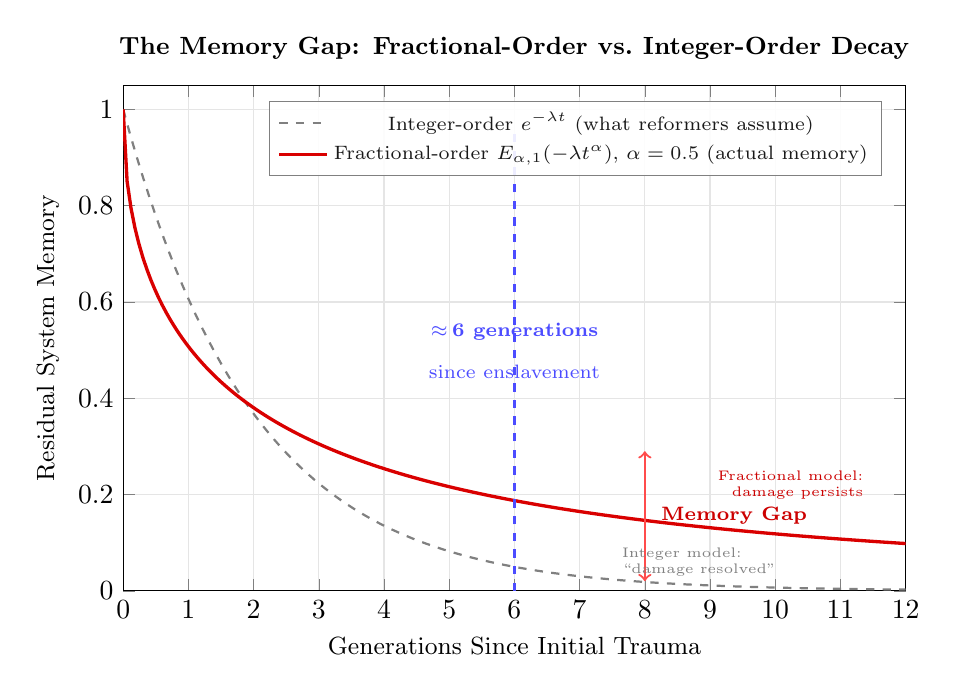
\begin{tikzpicture}
\begin{axis}[
    width=0.95\textwidth,
    height=8cm,
    xmin=0, xmax=12,
    ymin=0, ymax=1.05,
    xlabel={Generations Since Initial Trauma},
    ylabel={Residual System Memory},
    xlabel style={font=\small},
    ylabel style={font=\small},
    title={\textbf{The Memory Gap: Fractional-Order vs.\ Integer-Order Decay}},
    title style={font=\bfseries\small},
    legend style={at={(0.97,0.97)}, anchor=north east, font=\scriptsize, fill=white, fill opacity=0.9, draw=gray},
    grid=major,
    grid style={gray!20},
    xtick={0,1,...,12},
    ytick={0,0.2,0.4,0.6,0.8,1.0},
]

\addplot[dashed, thick, black!50, samples=120, domain=0:12]
    {exp(-0.5*x)};
\addlegendentry{Integer-order $e^{-\lambda t}$ (what reformers assume)}

\addplot[very thick, red!85!black, samples=200, domain=0:12]
    {1/(1 + 0.65*x^0.5 + 0.25*x + 0.06*x^1.5 + 0.01*x^2)};
\addlegendentry{Fractional-order $E_{\alpha,1}(-\lambda t^{\alpha})$, $\alpha=0.5$ (actual memory)}

\draw[thick, blue!70, dashed] (axis cs:6,0) -- (axis cs:6,0.95);
\node[anchor=south, font=\scriptsize\bfseries, text=blue!70] at (axis cs:6,0.50) {$\approx$\,6 generations};
\node[anchor=south, font=\scriptsize, text=blue!70] at (axis cs:6,0.42) {since enslavement};

\draw[<->, thick, red!70] (axis cs:8,0.02) -- (axis cs:8,0.29);
\node[anchor=west, font=\scriptsize\bfseries, text=red!80!black] at (axis cs:8.1,0.155) {Memory Gap};

\node[anchor=west, font=\tiny, text=black!50, align=left] at (axis cs:7.5,0.06) {Integer model:\\``damage resolved''};

\node[anchor=east, font=\tiny, text=red!80!black, align=right] at (axis cs:11.5,0.22) {Fractional model:\\damage persists};

\end{axis}
\end{tikzpicture}
\caption{\textbf{The Memory Gap: Why Historical Damage Persists.} Under standard integer-order dynamics ($\alpha = 1$), a system's memory of initial conditions decays exponentially---the implicit assumption behind reform timelines that measure progress in electoral cycles. Under fractional-order dynamics ($\alpha = 0.5$), the Mittag-Leffler function decays as a power law: the memory of initial trauma persists across generations, with the residual far exceeding the integer-order prediction at every time horizon. At generation~6 (approximately the present distance from the end of chattel slavery), the integer model registers near-zero residual memory; the fractional model registers substantial ongoing structural deformation. The Middle Passage is a permanent deformation of the state trajectory.}
\label{fig:memory_gap}
\end{figure}

As the Predatory Min-Max Function exhausts extraction from $O_{\text{racialized}}$, the same compounding logic eventually turns inward: the tools developed to diminish $O_{\text{racialized}}$ are redeployed against $I \setminus E$, whose own capacity then begins to compound downward (see Section~6.12).

\begin{figure}[htbp]
\centering
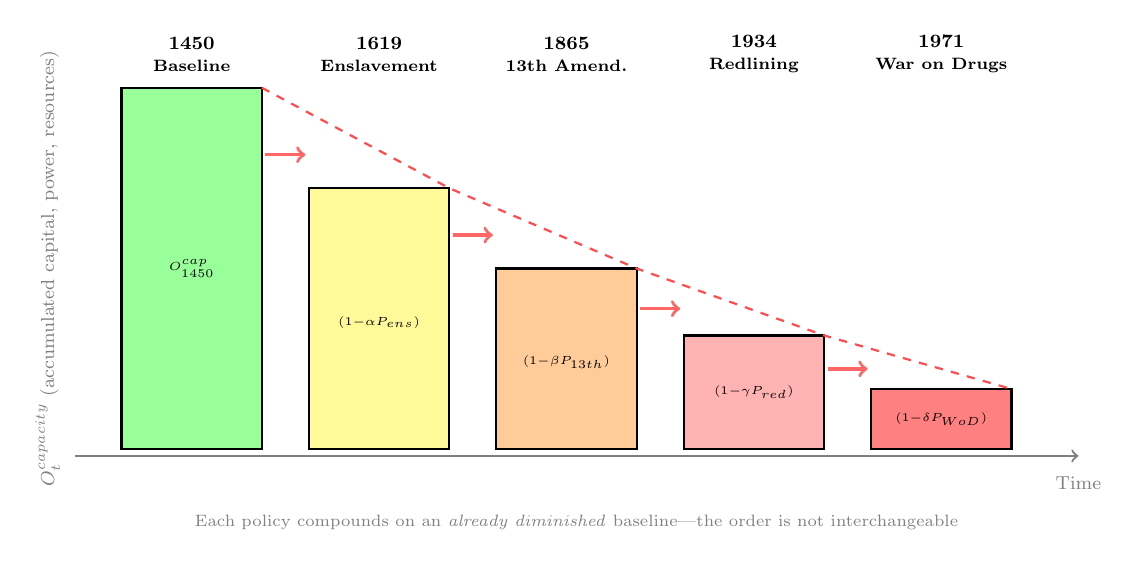
\begin{tikzpicture}[scale=0.85, transform shape]
    % Timeline axis
    \draw[->, thick, gray] (-0.5,0) -- (14.5,0);
    \node[gray, font=\footnotesize] at (14.5,-0.4) {Time};

    % Capacity bars (staircase of decline)
    % 1450 baseline
    \fill[green!40] (0.2,0.1) rectangle (2.3,5.5);
    \draw[thick] (0.2,0.1) rectangle (2.3,5.5);
    \node[font=\footnotesize\bfseries, align=center] at (1.25,6.0) {1450\\{\scriptsize Baseline}};
    \node[font=\tiny, align=center] at (1.25,2.8) {$O_{1450}^{\text{cap}}$};

    % 1619 after enslavement
    \fill[yellow!40] (3.0,0.1) rectangle (5.1,4.0);
    \draw[thick] (3.0,0.1) rectangle (5.1,4.0);
    \node[font=\footnotesize\bfseries, align=center] at (4.05,6.0) {1619\\{\scriptsize Enslavement}};
    \node[font=\tiny, align=center] at (4.05,2.0) {$(1{-}\alpha P_{\text{ens}})$};
    \draw[->, very thick, red!60] (2.35,4.5) -- (2.95,4.5);

    % 1865 after 13th Amendment
    \fill[orange!40] (5.8,0.1) rectangle (7.9,2.8);
    \draw[thick] (5.8,0.1) rectangle (7.9,2.8);
    \node[font=\footnotesize\bfseries, align=center] at (6.85,6.0) {1865\\{\scriptsize 13th Amend.}};
    \node[font=\tiny, align=center] at (6.85,1.4) {$(1{-}\beta P_{\text{13th}})$};
    \draw[->, very thick, red!60] (5.15,3.3) -- (5.75,3.3);

    % 1934 after redlining
    \fill[red!30] (8.6,0.1) rectangle (10.7,1.8);
    \draw[thick] (8.6,0.1) rectangle (10.7,1.8);
    \node[font=\footnotesize\bfseries, align=center] at (9.65,6.0) {1934\\{\scriptsize Redlining}};
    \node[font=\tiny, align=center] at (9.65,0.95) {$(1{-}\gamma P_{\text{red}})$};
    \draw[->, very thick, red!60] (7.95,2.2) -- (8.55,2.2);

    % 1971 after War on Drugs
    \fill[red!50] (11.4,0.1) rectangle (13.5,1.0);
    \draw[thick] (11.4,0.1) rectangle (13.5,1.0);
    \node[font=\footnotesize\bfseries, align=center] at (12.45,6.0) {1971\\{\scriptsize War on Drugs}};
    \node[font=\tiny, align=center] at (12.45,0.55) {$(1{-}\delta P_{\text{WoD}})$};
    \draw[->, very thick, red!60] (10.75,1.3) -- (11.35,1.3);

    % Declining envelope line
    \draw[dashed, thick, red!70] (2.3,5.5) -- (5.1,4.0) -- (7.9,2.8) -- (10.7,1.8) -- (13.5,1.0);

    % Y-axis label
    \node[rotate=90, font=\footnotesize, gray] at (-0.9,2.8) {$O_t^{\text{capacity}}$ (accumulated capital, power, resources)};

    % Bottom annotation
    \node[font=\scriptsize, align=center, gray] at (7.0,-1.0) {Each policy compounds on an \textit{already diminished} baseline---the order is not interchangeable};
\end{tikzpicture}
\caption{\textbf{The Staircase of Decline: Historical Compounding of Out-Group Capacity.} Each policy reduces $O_t^{\text{capacity}}$ multiplicatively. The bars show how each successive policy---enslavement (1619), the 13th Amendment loophole (1865), redlining (1934), and the War on Drugs (1971)---compounds on an already diminished baseline, making the present condition of $O_{\text{racialized}}$ a mathematical inevitability of the policy sequence.}
\label{fig:historical_compounding}
\end{figure}

\begin{figure}[htbp]
\centering
\begin{tikzpicture}[every node/.style={font=\small}]
    % Capacity boxes
    \node[draw, thick, fill=green!30, minimum width=3cm, minimum height=2.8cm] (o0) at (0,0) {$O_0^{\text{capacity}}$};
    \node[draw, thick, fill=yellow!25, minimum width=3cm, minimum height=2.8cm, right=3.8cm of o0] (o1) {$O_1^{\text{capacity}}$};
    \node[draw, thick, fill=orange!30, minimum width=3cm, minimum height=2.8cm, right=3.8cm of o1] (o2) {$O_2^{\text{capacity}}$};

    % Capacity equations
    \node[font=\footnotesize] at ($(o1)+(0,-0.7)$) {$=\, O_0 \cdot (1-\alpha P_1)$};
    \node[font=\footnotesize] at ($(o2)+(0,-0.7)$) {$=\, O_1 \cdot (1-\beta P_2)$};

    % Policy arrows
    \draw[->, very thick, red] (o0.east) -- (o1.west);
    \draw[->, very thick, red] (o1.east) -- (o2.west);
    \node[red, font=\normalsize, align=center] at ($(o0)!0.5!(o1)+(0,1.0)$) {Policy $P_1$\\\footnotesize(enslavement)};
    \node[red, font=\normalsize, align=center] at ($(o1)!0.5!(o2)+(0,1.0)$) {Policy $P_2$\\\footnotesize(redlining)};

    % Time labels
    \node[font=\normalsize] at ($(o0)+(0,-1.9)$) {Time $t=0$};
    \node[font=\normalsize] at ($(o0)+(0,-2.35)$) {(initial)};

    \node[font=\normalsize] at ($(o1)+(0,-1.9)$) {Time $t=1$};
    \node[font=\normalsize, red] at ($(o1)+(0,-2.35)$) {(diminished)};

    \node[font=\normalsize] at ($(o2)+(0,-1.9)$) {Time $t=2$};
    \node[font=\normalsize, red] at ($(o2)+(0,-2.35)$) {(compounded)};

    % Visual representation of shrinking
    \draw[<->, thick, blue] ($(o0)+(-1.55,-3)$) -- ($(o0)+(1.55,-3)$);
    \node[blue, font=\normalsize] at ($(o0)+(0,-3.25)$) {Full capacity};

    \draw[<->, thick, blue] ($(o1)+(-1.55,-3)$) -- ($(o1)+(1.55,-3)$);
    \node[blue, font=\normalsize] at ($(o1)+(0,-3.25)$) {Reduced};

    \draw[<->, thick, blue] ($(o2)+(-1.55,-3)$) -- ($(o2)+(1.55,-3)$);
    \node[blue, font=\normalsize] at ($(o2)+(0,-3.25)$) {Severely reduced};

    % Annotation
    \node[align=center, font=\small] at ($(o1)+(0,-4.55)$) {$P_2$ applied to \textit{already diminished} group\\$\Rightarrow$ compounding harm, not additive};
\end{tikzpicture}
\caption{Temporal compounding model: Each policy reduces Out-group capacity, making subsequent policies more harmful. Policy $P_2$ (redlining) causes greater harm when applied to a group already diminished by $P_1$ (enslavement). As the system exhausts extraction from $O_{\text{racialized}}$, this same compounding mechanism is eventually turned against $I \setminus E$ (Section~6.12).}
\label{fig:compounding}
\end{figure}

\begin{figure}[htbp]
\centering
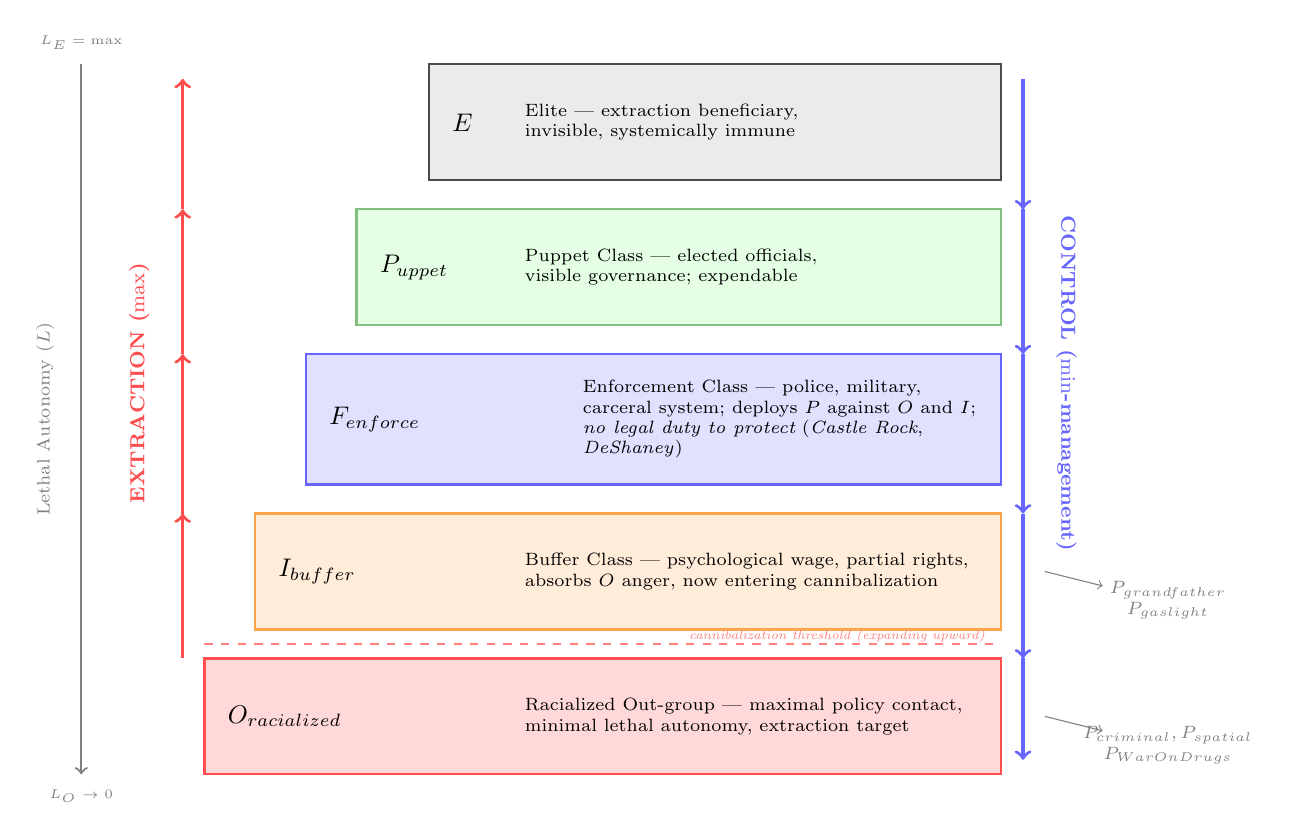
\begin{tikzpicture}[scale=0.92, transform shape]
    % --- Tier boxes (bottom to top = O to E) ---
    % Left edges stagger inward (pyramid shape); right edges align at 5.5 to contain text
    % O_racialized (bottom, widest)
    \fill[red!15] (-5.5,-0.4) rectangle (5.5,1.2);
    \draw[thick, red!70] (-5.5,-0.4) rectangle (5.5,1.2);
    \node[font=\bfseries, anchor=west] at (-5.3,0.4) {$O_{\text{racialized}}$};
    \node[font=\scriptsize, align=left, anchor=west] at (-1.2,0.4) {Racialized Out-group --- maximal policy contact,\\minimal lethal autonomy, extraction target};

    % I_buffer
    \fill[orange!15] (-4.8,1.6) rectangle (5.5,3.2);
    \draw[thick, orange!70] (-4.8,1.6) rectangle (5.5,3.2);
    \node[font=\bfseries, anchor=west] at (-4.6,2.4) {$I_{\text{buffer}}$};
    \node[font=\scriptsize, align=left, anchor=west] at (-1.2,2.4) {Buffer Class --- psychological wage, partial rights,\\absorbs $O$ anger, now entering cannibalization};

    % F_enforce
    \fill[blue!12] (-4.1,3.6) rectangle (5.5,5.4);
    \draw[thick, blue!60] (-4.1,3.6) rectangle (5.5,5.4);
    \node[font=\bfseries, anchor=west] at (-3.9,4.5) {$F_{\text{enforce}}$};
    \node[font=\scriptsize, align=left, anchor=west] at (-0.4,4.5) {Enforcement Class --- police, military,\\carceral system; deploys $P$ against $O$ and $I$;\\{\itshape no legal duty to protect} (\textit{Castle Rock},\\\textit{DeShaney})};

    % P_uppet
    \fill[green!10] (-3.4,5.8) rectangle (5.5,7.4);
    \draw[thick, green!50!black!50] (-3.4,5.8) rectangle (5.5,7.4);
    \node[font=\bfseries, anchor=west] at (-3.2,6.6) {$P_{\text{uppet}}$};
    \node[font=\scriptsize, align=left, anchor=west] at (-1.2,6.6) {Puppet Class --- elected officials,\\visible governance; expendable};

    % E (top, narrowest left edge but extends right to contain text)
    \fill[black!8] (-2.4,7.8) rectangle (5.5,9.4);
    \draw[thick, black!70] (-2.4,7.8) rectangle (5.5,9.4);
    \node[font=\bfseries, anchor=west] at (-2.2,8.6) {$E$};
    \node[font=\scriptsize, align=left, anchor=west] at (-1.2,8.6) {Elite --- extraction beneficiary,\\invisible, systemically immune};

    % --- Extraction arrows (upward, left side) ---
    \draw[->, very thick, red!70] (-5.8,1.2) -- (-5.8,3.2);
    \draw[->, very thick, red!70] (-5.8,3.2) -- (-5.8,5.4);
    \draw[->, very thick, red!70] (-5.8,5.4) -- (-5.8,7.4);
    \draw[->, very thick, red!70] (-5.8,7.4) -- (-5.8,9.2);
    \node[rotate=90, font=\footnotesize\bfseries, red!70] at (-6.4,5.0) {EXTRACTION ($\max$)};

    % --- Control arrows (downward, right side) ---
    \draw[->, very thick, blue!60] (5.8,9.2) -- (5.8,7.4);
    \draw[->, very thick, blue!60] (5.8,7.4) -- (5.8,5.4);
    \draw[->, very thick, blue!60] (5.8,5.4) -- (5.8,3.2);
    \draw[->, very thick, blue!60] (5.8,3.2) -- (5.8,1.2);
    \draw[->, very thick, blue!60] (5.8,1.2) -- (5.8,-0.2);
    \node[rotate=270, font=\footnotesize\bfseries, blue!60] at (6.4,5.0) {CONTROL ($\min$-management)};

    % --- Policy variable annotations (right side, between tiers) ---
    \node[font=\scriptsize, gray, align=center] at (7.8,0.0) {$P_{\text{criminal}}, P_{\text{spatial}}$\\$P_{\text{WarOnDrugs}}$};
    \draw[->, thin, gray] (6.1,0.4) -- (6.9,0.2);

    \node[font=\scriptsize, gray, align=center] at (7.8,2.0) {$P_{\text{grandfather}}$\\$P_{\text{gaslight}}$};
    \draw[->, thin, gray] (6.1,2.4) -- (6.9,2.2);

    % --- Lethal autonomy gradient (far left) ---
    \draw[<-, thick, black!50] (-7.2,-0.4) -- (-7.2,9.4);
    \node[rotate=90, font=\scriptsize, black!50] at (-7.7,4.5) {Lethal Autonomy ($L$)};
    \node[font=\tiny, black!50] at (-7.2,-0.7) {$L_O \to 0$};
    \node[font=\tiny, black!50] at (-7.2,9.7) {$L_E = \max$};

    % --- Cannibalization zone annotation ---
    \draw[thick, dashed, red!50] (-5.5,1.4) -- (5.5,1.4);
    \node[font=\tiny\itshape, red!50, anchor=east] at (5.4,1.5) {cannibalization threshold (expanding upward)};

\end{tikzpicture}
\caption{\textbf{The 5-Tier Extraction Hierarchy.} The Predatory Min-Max Function operates through five nested tiers. Extraction ($\max$) flows upward from $O_{\text{racialized}}$ to $E$; control ($\min$-management) flows downward through policy variables ($P$) deployed by $F_{\text{enforce}}$ at the direction of $P_{\text{uppet}}$, which is itself expendable to $E$. Lethal autonomy increases from bottom to top. The dashed line marks the cannibalization threshold: as extraction exhausts $O_{\text{racialized}}$, the system expands its extraction zone upward into $I_{\text{buffer}}$, consuming the Buffer Class it originally created to protect itself.}
\label{fig:venn_model}
\end{figure}

This five-tier structure (Figure~\ref{fig:venn_model}) maps the full architecture of the Predatory Min-Max Function: extraction flows upward from the racialized Out-group to the Elite, while control flows downward through policy variables deployed by the Enforcement Class. The cannibalization threshold marks the system's current phase---expanding extraction beyond $O_{\text{racialized}}$ into the Buffer Class itself.

\section{The Unbroken Financial Lineage: From Slave Mortgages to Carceral Bonds}

The 13th Amendment's variable swap from racial identity to criminal status preserved an entire financial architecture. To understand the continuity, we must trace the capital pipeline from its antebellum origin.

That prison labor remains a federally regulated commodity---not a historical footnote---is visible in \usclink{apx:usc:18:1761}{18 U.S.C.~\S~1761}, which governs the interstate commerce of goods manufactured by convicts:
\uscinline{usc_18_1761}

Northern banks, insurance companies, and merchants profited enormously from financing and insuring the slave trade and slave-based production. Bonnie Martin's analysis of nearly 9,000 antebellum mortgages found that \textbf{47 percent involved enslaved human beings as collateral} \cite{martin}---revealing that the mortgage of human property was the \textit{invisible engine} of Southern capital formation.

The most striking case is that of \textbf{Citizens Bank and Canal Bank of Louisiana}, which collectively accepted approximately 13,000 enslaved people as mortgage collateral and directly owned more than 1,200 human beings \cite{baptist, murphy}. In 1836, the State of Louisiana issued \textbf{state-backed bonds} collateralized by these slave mortgages and marketed them to investors across Europe---through firms such as Baring Brothers in London, Amsterdam, and Paris. These instruments were, in function, \textbf{mortgage-backed securities} whose underlying ``assets'' were human beings. Both banks are now predecessor institutions of JPMorgan Chase.

This financial architecture did not disappear with the 13th Amendment---it \textit{evolved}. By 1860, enslaved people represented the largest single asset class in the United States, worth more than all manufacturing and railroads combined \cite{baptist, beckert}. The 13th Amendment rerouted this capital through the carceral system.

To see the continuity, we must trace the complete cash-flow pipeline in both eras and demonstrate that the \textit{string}---the unbroken thread connecting human body to financial instrument to investor---has been re-encoded at every stage.

\subsection{The Old String: Slave-Backed Securities (1830s--1865)}

The antebellum pipeline operated as follows:

\begin{enumerate}
    \item \textbf{The Asset}: An enslaved human being, legally classified as moveable property.
    \item \textbf{The Collateralization}: The enslaved person is mortgaged---pledged as collateral for a loan. Martin documents that 47\% of antebellum mortgages involved enslaved people as collateral \cite{martin}.
    \item \textbf{The Securitization}: Banks bundle these slave mortgages into state-backed bonds. Louisiana issues bonds collateralized by the slave portfolios of Citizens Bank and Canal Bank, marketed through Baring Brothers to investors in London, Amsterdam, and Paris \cite{murphy}.
    \item \textbf{The State Guarantee}: The state backs the instruments---its full faith and credit standing behind the return on investment.
    \item \textbf{The Revenue Stream}: The investor receives a guaranteed return. The return is generated by the labor extracted from the enslaved person's body.
    \item \textbf{The Enforcement}: Slave patrols ($F_{\text{enforce}}^{\text{v1.0}}$) function as \textit{asset recovery agents}---retrieving runaways (lost assets), suppressing revolts (protecting the portfolio), and maintaining the labor discipline that generates the revenue stream backing the bonds.
\end{enumerate}

The cash flow is: \textbf{Body $\rightarrow$ Labor $\rightarrow$ Revenue $\rightarrow$ Bond $\rightarrow$ Investor}. The state guarantees the instrument. The Enforcement Class protects the asset. The Elite in Europe sips tea while the return-on-investment is generated by the lash.

\subsection{The New String: Carceral Bonds (1983--Present)}

The modern pipeline replicates this structure with updated variable names:

\begin{enumerate}
    \item \textbf{The Asset}: An incarcerated human being, legally reclassified from ``slave'' to ``inmate'' via the 13th Amendment's exception clause.
    \item \textbf{The Collateralization}: Private prison companies (CoreCivic, GEO Group) issue bonds and revenue instruments whose value depends on maintaining incarcerated populations \cite{alexander}. Each occupied bed generates a per-diem payment from the state---typically \$50--\$150 per day per inmate.
    \item \textbf{The Securitization}: These revenue streams are packaged into financial instruments---corporate bonds, REITs (Real Estate Investment Trusts), and equity offerings---traded on public markets. CoreCivic and GEO Group are publicly traded on the New York Stock Exchange.
    \item \textbf{The State Guarantee}: Private prison contracts contain \textbf{occupancy guarantee clauses}---typically requiring the state to maintain \textbf{80--90\% bed occupancy} or pay for the empty beds regardless \cite{itpi}. The state's full faith and credit once again backs the instrument. If the beds are not filled with bodies, the taxpayer pays the difference.
    \item \textbf{The Revenue Stream}: The investor receives a guaranteed return. CoreCivic reported \$1.99 billion in revenue in 2022; GEO Group reported \$2.42 billion. These are not abstract financial numbers---they are the monetized output of human incarceration.
    \item \textbf{The Enforcement}: Police ($F_{\text{enforce}}$) function as \textit{asset acquisition agents}---filling the beds that back the bonds, meeting the quotas that satisfy the occupancy clauses, generating the bodies that produce the revenue stream that pays the investors.
\end{enumerate}

The cash flow is identical: \textbf{Body $\rightarrow$ Incarceration $\rightarrow$ Revenue $\rightarrow$ Bond $\rightarrow$ Investor}. The state guarantees the instrument. The Enforcement Class acquires the asset. The variable names changed; the string remained continuous.

\subsection{The Demand Signal: How Financial Instruments Manufacture Crime}

The occupancy guarantee clause is the load-bearing variable that converts the carceral system into a \textit{demand-driven asset pipeline}. Trace the causal chain:

\begin{enumerate}
    \item $E$ (the Elite) invests in private prison bonds, expecting a 7--10\% annual return.
    \item The return depends on beds being occupied. The private prison contract guarantees 90\% occupancy.
    \item The state must deliver bodies to fill those beds---or pay for the empty ones.
    \item The state directs $F_{\text{enforce}}$ (police departments) to meet arrest quotas calibrated to the occupancy requirements.
    \item $F_{\text{enforce}}$ requires a legal mechanism to generate arrests at scale. The Puppet Class ($P_{\text{uppet}}$) has already provided one: the legislative web of Universal Latent Criminality documented in Chapter~\ref{ch:full_algo}. The average American commits an estimated three felonies per day without knowing it \cite{silverglate}. The law is written so broadly that \textit{everyone} is a potential arrest---the system merely selects \textit{which} bodies to process.
    \item $F_{\text{enforce}}$ exercises selective enforcement---choosing from the full glossary of available charges to fill the beds. The selection is not random. It follows the path of least resistance: $O_{\text{racialized}}$ first (the population with the least political and legal capital to resist), then the lower strata of $I_{\text{buffer}}$ as the extraction zone expands.
\end{enumerate}

This is why the police have \textit{no legal duty to protect you} (Castle Rock, DeShaney). They were never designed to protect. They were designed---from the slave patrols of the 18th century to the quota-driven departments of the 21st---to \textit{acquire and maintain assets} for the financial instruments that sit at the top of the extraction pipeline. The ``no duty to protect'' doctrine is the system telling you, through its own case law, exactly what $F_{\text{enforce}}$ was built to do.

The demand signal flows \textit{downward} through the hierarchy: $E$ demands returns $\rightarrow$ private prisons demand bodies $\rightarrow$ state guarantees occupancy $\rightarrow$ police departments enforce quotas $\rightarrow$ prosecutors stack charges $\rightarrow$ bodies enter the pipeline. The supply of ``crime'' is manufactured to meet the demand of capital. This is a market, not a conspiracy. The incarcerated human being is the commodity. The bond is the instrument. The state is the guarantor. The police are the supply chain.

And here is the structural revelation: \textit{the string has never been cut}. From the 1836 Louisiana slave bond purchased by a London banker to the 2026 CoreCivic corporate bond purchased by a hedge fund manager, the pipeline is continuous. A human body enters the system. Its captivity generates revenue. That revenue is securitized into a financial instrument. The instrument is sold to an investor. The investor receives a return. The Enforcement Class ensures the supply. The state guarantees the product.

The only thing that changed was the legal classification of the body at the point of entry. The 13th Amendment's ``except as a punishment for crime'' clause \textit{privatized the front end and securitized the back end}. The rest of the string---from body to bond to investor---remained structurally, financially, and morally identical.

\subsection{The Triple Conversion: Labor, Census Weight, and Voiceless Population}

The modern carceral subject is converted by the system into three simultaneous assets. First, the body becomes \textbf{labor input}. ACLU and University of Chicago researchers estimate that incarcerated workers generate at least \$2 billion in goods and \$9 billion in prison-maintenance services each year, while 76\% of surveyed incarcerated workers report punishment for refusing or being unable to work \cite{aclu_captive_labor_2022}. The punishment exception is therefore not symbolic. It supplies the legal interface through which coerced labor reappears as ``work programming,'' kitchen duty, laundry, maintenance, road work, firefighting, and public-service labor.

Second, the body becomes an \textbf{institutional-maintenance subsidy}. As the incarcerated population ages, younger prisoners become more valuable to the prison as the labor force that keeps the facility itself operating. The aging trend is measurable: Prison Policy Initiative reports that people age 55 and older rose from 3.4\% of the prison population in 1991 to 15.3\% in 2021, and that 30\% of people serving life sentences were at least 55 years old by 2020 \cite{ppi_aging_prisons_2023}. Life sentences therefore create a long-duration labor reservoir inside an institution whose own maintenance demands rise as the captive population ages.

Third, the body becomes \textbf{census population}. Prison gerrymandering counts incarcerated people where they are confined, apart from the communities from which they were removed, inflating the representational weight and demographic profile of prison-hosting jurisdictions while the incarcerated people themselves remain politically powerless there \cite{brennan_prison_gerrymandering_2025, redistrictingdatahub_prison_gerrymandering}. This can radically distort local population counts: Prisoners of the Census identified nearly forty municipalities where prisons account for more than half the reported census population, including Ina, Illinois, where incarcerated people comprised roughly 80\% of the municipal count \cite{prisoners_census_municipal_2020}.

This is the fully compiled form of $P_{\text{criminal}} + P_{\text{spatial}}$. The incarcerated person is economically useful, administratively necessary, and politically countable, while being severed from the political agency that normally attaches to personhood. The same body is extracted as labor, used as fiscal and maintenance infrastructure, and then redeployed as representational mass for jurisdictions that do not represent it. The carceral state thus performs a triple conversion: \textbf{body $\rightarrow$ labor input}; \textbf{body $\rightarrow$ institutional subsidy}; \textbf{body $\rightarrow$ census weight}. The subject becomes valuable everywhere except at the point of citizenship.

\section{Imperial Enforcement: The 1915 Occupation and the Resurrection of the Corv\'{e}e}
\label{sec:haiti_occupation}

To understand the full scope of the Buffer Class's enforcement role, one must examine how the Elite deploys nominal In-group members across sovereign borders. The United States occupation of Haiti (1915–1934) perfectly models the corporate weaponization of the state. The pre-1915 arc---Haiti's material export of liberation to Gran Colombia, Mexico, the Dominican Republic, and Greece; the vexillological encoding of revolutionary solidarity; and the Firmin Protocol's 1891 diplomatic repulsion of U.S. naval coercion---is documented in Chapter~\ref{ch:haitian_export}. The 1915 occupation represents the Elite's recursive answer to that full counter-strategy: when the financial and legal mechanisms proved insufficient to neutralize $O_{\text{emancipated}}$'s institutional capacity, the enforcement mechanism was deployed in its most direct form.

The occupation was driven by the financial imperatives of the American Elite, specifically Wall Street institutions like National City Bank (now Citibank). The US military—functioning as the ultimate, transnational manifestation of the slave patrol—was deployed to seize Haiti's gold reserves, commandeer its customs houses, and forcibly rewrite its constitution to allow foreign land ownership.

Once in control, the occupying forces immediately reinstated the \textit{corv\'{e}e}, a system of forced, unpaid labor utilized to build infrastructure for the benefit of foreign corporate interests. This demonstrates the algorithmic consistency of the Elite's operating system. Just as the 13th Amendment loophole was utilized domestically to re-enslave Black Americans through the carceral state, the US military utilized imperial law to institute forced labor upon the Haitian population. The extraction of Black labor for the benefit of white capital ($E$) was forcefully resumed, masked entirely behind the ideological justification (Component 3) of ``modernization'' and ``civilization.''

\section{The Geographic Displacement of Slave Capitalism}

The Haitian occupation reveals a broader structural truth: \textbf{industrial capitalism \textit{is} slave capitalism}---evolved and geographically dispersed. Formal abolition changed the legal form and location of slavery, leaving the extraction kernel intact. After centuries of extracting African bodies as slaves, capitalism now extracts African labor \textit{in situ}---keeping the exploitation in Africa while extracting the value. Former colonial powers use structural adjustment, debt, and military coercion to maintain exploitative relationships that replicate the extraction kernel across sovereign borders.

\subsection{Case Study: France's Dependence on African Exploitation}

The contemporary crisis in French-African relations exposes this dependency with mathematical precision. France's economy has long relied on:

\begin{itemize}
    \item \textbf{CFA Franc system}: 14 African nations forced to use currency controlled by the French Treasury, required to deposit 50--85\% of their reserves in France \cite{pigeaud}, giving France de facto control over their monetary policy
    \item \textbf{Resource extraction contracts}: Uranium from Niger powers French nuclear plants (70\% of French electricity); France pays far below market rates under contracts established during the colonial period
    \item \textbf{Military enforcement}: France maintains military bases across former colonies to protect these arrangements, intervening militarily whenever governments attempt to renegotiate
\end{itemize}

As of 2023--2024, multiple African nations (Niger, Mali, Burkina Faso, Gabon) have expelled French military, rejected the CFA Franc, and nationalized resources. France's economy is experiencing serious strain---energy crisis, loss of captive markets, capital flight, and inflation from paying market rates for resources previously extracted at colonial prices. This demonstrates the dependency of \textbf{Western industrial capitalism on access to exploited African labor and resources}. The system is slavery with updated public relations.

The extraction function remains continuous: the ``asset class'' changed its legal designation from ``slave'' to ``debtor nation''; the Predatory Min-Max Function remained intact. The Elite ($E$) traces an unbroken financial lineage from antebellum planters who securitized enslaved bodies, to colonial administrators who extracted resources through military occupation, to modern multinational corporations that extract through debt instruments and trade agreements. The variable $E$ has merely globalized; the kernel has never been modified.

\begin{keyinsight}[Hardware Reading: The Current Source and the One-Way Diode]
The Enforcement Engine is the \textbf{current source} of the extraction circuit: it dictates the direction and magnitude of enforcement flow, independent of the load's resistance. Slave patrols were the prototype---armed white men conscripted into $F_{\text{enforce}}$ to maintain current direction toward $O_{\text{racialized}}$. The 13th Amendment's exception clause (``except as a punishment for crime'') was a \textbf{P-N junction diode} installed at the exact moment the capacitor of chattel slavery was discharged: it ensured that current could still flow \emph{into} the carceral state even when it could no longer flow through the property-law branch. The Fugitive Slave Act (1850) was a \textbf{reverse-bias protection circuit}: it prevented any state from blocking the federal enforcement current. The compounding model documented in this chapter---patrols $\rightarrow$ militias $\rightarrow$ police $\rightarrow$ prisons---is the same current source, operating through successively more efficient transistor topologies, all serving the same $V_{cc}$ rail: the kinetic labor, tax base, and physical output of the Out-group and Buffer Class.
\end{keyinsight}

\part{Scaling and Runtime (1865--Present)}
\label{part:runtime}

\chapter{The Containment: Pullman, Redlining, and the Wages of Whiteness (1894--1965)}
\label{ch:containment}

\begin{tcolorbox}[colback=black!5, colframe=black!70, fonttitle=\bfseries\ttfamily, title=RUNTIME LOG: 1894--1965 (POST-EMANCIPATION CONTAINMENT)]
\ttfamily\small
\textbf{System Stress} ($\min$: class resistance): HIGH --- 13th Amendment reclassified $O_{\text{racialized}}$ as citizens with voting rights. Parallel Out-group economy emerging. Civil Rights Movement breaching the legal interface.\\
\textbf{Capital} ($\max$: extraction output): RESTRUCTURING --- Direct slavery terminated. System transitioning to indirect extraction via convict leasing, sharecropping, and spatial containment.\\
\textbf{Interference State} ($\Phi_{\text{load}}$, proximity to $\tau$): $\Phi_{\text{load}} \in [0.55, 0.72]$; $\rho_{\tau} \in [0.50, 0.68]$.\\
\textbf{Variables Loaded}: $E$, $O_{\text{racialized}}$, $I$, $I_{\text{buffer}}$, $F_{\text{enforce}}$.\\
\textbf{Variables Deployed This Cycle}: $W$ (Complex Wage, weaponized), $P_{\text{spatial}}$ (Redlining), Capture Variable.\\
\textbf{Executing Function}: Terminate the Out-group's parallel economy (Tulsa 1921, East St.\ Louis 1917). Build the containment field $P_{\text{spatial}}$ (National Housing Act 1934). Absorb the Civil Rights Movement's legal victories into two-party loyalty without dismantling the extraction kernel.\\
\textbf{Result}: \textbf{[POLICY]} HOLC Redlining (1934) concentrates $O_{\text{racialized}}$ for targeted extraction. \textbf{[POLICY]} Civil Rights Act (1964) and Voting Rights Act (1965) dismantle the legal interface but leave the kernel untouched. Capture Variable absorbs $O_{\text{racialized}}$ into the two-party system. $\min$ restored through spatial and political containment. The Puppet Class upgrade that coordinates these moves is deployed in Chapter~\ref{ch:tweedism}.
\end{tcolorbox}

\medskip

The 13th Amendment terminated direct slavery. Extraction continued, and the Elite ($E$) needed a containment architecture that could hold a newly enfranchised Out-group ($O_{\text{racialized}}$) inside the extraction zone without the explicit legal interface of chattel ownership. This chapter traces three moves that built that architecture: (i) the 1894 Pullman Strike, in which the Buffer Class's investment in the psychological wage ($\psi$) destroyed the one labor coalition that could have toppled industrial capital; (ii) the 1917--1934 kinetic and legal operations---Tulsa, East St.\ Louis, the National Housing Act---that terminated the Out-group's parallel economy and compressed it into redlined containment fields; and (iii) the mid-twentieth-century Capture Variable, through which the Civil Rights Movement's legal victories were absorbed into two-party political loyalty without disturbing the extraction kernel. Chapter~\ref{ch:tweedism} then takes up the democratic front-end that coordinates these moves: the industrialized Puppet Class ($P_{\text{uppet}}$) and the Tweedism Filter.

Containment gives the mind virus a map. Redlining, sundown towns, school boundaries, restrictive covenants, and urban-renewal clearance trained perception by making race, risk, poverty, policing, and property value appear to occupy the same coordinates. The host wetware then learned the geography as if it were evidence: this neighborhood is dangerous, that school is failing, this applicant is risky. Spatial policy became cognitive firmware.

The deeper context for this chapter is provided by Du Bois's analytical architecture in \textit{Black Reconstruction} \cite{dubois}. Du Bois argued that Reconstruction (1865--1877) constituted a successful multiracial democracy that was \textit{overthrown} by a coordinated counter-revolution of property. The critical mechanism was Northern capital's recognition that the Reconstruction governments' labor and land reforms threatened industrial extraction at the national scale. The railroad magnates, industrial financiers, and Northern Republican machine that had fought to end slavery quickly made common cause with Southern Redeemer Democrats the moment Black political power threatened to raise labor standards and redistribute land. Du Bois named this the ``counter-revolution of property'': the restoration of the extraction kernel through elite-class alliance across the racial partition the Elite had previously used to divide the laboring class. This chapter's three case studies---Pullman, redlining, and the Capture Variable---are the post-1877 continuation of that counter-revolution: the same Elite interest in containing cross-racial democracy, now operating through capital after the paramilitary phase.

We begin with the Gilded Age's most elegant proof that the Buffer Class's investment in $\psi$ is \textit{self-defeating}---a case where the white working class's refusal to organize across the racial partition handed the Elite the precise weapon needed to destroy them.

\section{The Pullman Strike: How the Psychological Wage Broke the Working Class (1894)}

In 1894, the Pullman Palace Car Company---manufacturer of the luxury sleeping cars that defined American rail travel---slashed wages by 25 percent while refusing to reduce rents in the company town of Pullman, Illinois, where workers were compelled to live. Workers who earned \$9 per week received paychecks of \$0.07 after rent was deducted. The material conditions were objectively intolerable \cite{lindsey_pullman, salvatore_debs}.

Eugene V. Debs, leader of the newly formed American Railway Union (ARU), organized a national boycott: ARU members across the country refused to handle any train with a Pullman car attached. Within days, rail traffic across 27 states ground to a halt. Railroad profits collapsed. The strike was \textit{working}.

Here is where the popular narrative---recently recirculated through social media---claims that this was ``America's first successful integrated strike,'' with Black Pullman porters and white railroad workers standing together in unified action. \textbf{This is historically false, and the actual record is far more damning.}

The ARU was a \textbf{whites-only union}. At its 1893 founding convention, the membership voted to restrict enrollment to white railroad employees, overriding Debs's personal objections \cite{salvatore_debs, arnesen_waterfront}. Black workers---including the Pullman porters who suffered under some of the most exploitative conditions in the industry---were categorically excluded from the organization that claimed to represent all railroad labor.\footnote{Du Bois had already diagnosed this structural pathology in \textit{Black Reconstruction} \cite{dubois}, tracing the same dynamic through the collapse of the Knights of Labor in the 1880s. The Knights briefly admitted Black workers on an integrated basis; the AFL's founding in 1886 reversed that policy, institutionalizing craft-union exclusion at precisely the moment when industrial unionism could have built durable cross-racial power. The ARU's 1893 exclusion was not a new error---it was the same capitulation to $\psi$ that Du Bois had already identified as the primary mechanism by which white labor forfeited its material leverage to Elite capital.}

Within the framework, this is the psychological wage ($\psi$) operating at the institutional level. The white working class was offered a choice: build a union that included $O_{\text{racialized}}$ and maximize collective bargaining power, or build a union that excluded $O_{\text{racialized}}$ and preserve racial status hierarchy. They chose $\psi$. They chose whiteness over power.

\subsection{Capital Weaponizes the Partition}

The Elite ($E$)---organized through the \textbf{General Managers' Association (GMA)}, a consortium of 24 railroad companies---immediately exploited the racial partition the ARU had built into its own architecture. The GMA actively recruited Black workers as strikebreakers, offering the very jobs the ARU had refused to share \cite{arnesen_waterfront, lindsey_pullman}.

The mathematical logic was devastating:
\begin{enumerate}
    \item The ARU excluded Black workers from the union ($O_{\text{racialized}} \notin \text{ARU}$).
    \item Black workers therefore had zero institutional loyalty to the strike and rational economic incentive to accept replacement positions.
    \item The GMA deployed excluded Black workers to cross picket lines, simultaneously breaking the strike \textit{and} inflaming the racial resentment that had produced the exclusion in the first place.
\end{enumerate}

The Elite exploited a racial division that the Buffer Class had pre-installed. Capital merely \textit{weaponized} it. This is the framework's prediction operating in real time: the psychological wage ($\psi$) accepted by $I_{\text{buffer}}$ in exchange for policing the racial boundary is a \textit{vulnerability} that $E$ exploits whenever class solidarity threatens extraction.

\subsection{The Manufactured Pretext: Mail Cars as Legal Fiction}

Even with strikebreakers deployed, the boycott was paralyzing the national rail system. The Elite required federal force. But there was a constitutional obstacle: Illinois Governor John Peter Altgeld---a progressive who understood the strike as a legitimate labor action---explicitly refused to request federal intervention, insisting that the state was fully capable of maintaining order \cite{lindsey_pullman}.

President Grover Cleveland had no constitutional invitation to act. The Puppet Class ($P_{\text{uppet}}$) needed a pretext.

The solution was architecturally elegant. The GMA \textit{deliberately attached Pullman passenger cars to trains carrying U.S.\ mail}. This constituted a calculated maneuver to ensure that any boycott of Pullman cars would simultaneously obstruct federal mail delivery. The railroad managers manufactured the very federal crisis they then asked the government to resolve \cite{lindsey_pullman, papke_pullman}.

Attorney General Richard Olney---himself a \textbf{former board member of multiple railroad companies} and a man who continued to receive a retainer from the Burlington Railroad while serving as the nation's chief law enforcement officer---secured a blanket federal injunction under the Sherman Antitrust Act, prohibiting Debs and the ARU from ``compelling or encouraging'' any interference with rail operations \cite{papke_pullman, salvatore_debs}.

The irony is structurally perfect: the Sherman Antitrust Act, ostensibly designed to prevent \textit{corporate} monopolies from crushing competition, was repurposed by a corporate attorney serving as Attorney General to crush a \textit{labor} union. The statute designed to restrain $E$ was deployed by $P_{\text{uppet}}$ to protect $E$. The interface was rewritten in real time.

\subsection{12,000 Troops: The Enforcement Class Protects Capital}

On July 3, 1894, President Cleveland deployed approximately 12,000 federal troops to Chicago under the command of Brigadier General Nelson Miles---over Governor Altgeld's furious written protest that the action was ``a violation of a basic principle of our institutions'' \cite{lindsey_pullman}.

The troops' stated mission was protecting mail delivery. Their actual operations told a different story: they guarded railroad property, escorted strikebreakers to their positions, and cleared workers from rail yards. The Enforcement Class ($F_{\text{enforce}}$) was executing capital protection under the legal fiction of postal security.

The strike collapsed. Debs was arrested, convicted of contempt for violating the injunction, and imprisoned. The Supreme Court, in \textit{In re Debs} (1895), unanimously upheld the federal government's authority to intervene, ruling that the government's power over interstate commerce and mail delivery justified the injunction regardless of whether state authorities had requested assistance \cite{inredebs}.

The judicial branch of $P_{\text{uppet}}$ retroactively blessed the entire operation. The precedent was set: when labor organization threatened capital extraction, the federal government could bypass state authority, deploy military force, and imprison labor leaders---all under manufactured legal pretexts validated after the fact by compliant courts.

\subsection{The Theorem the Buffer Class Refused to Learn}

The Pullman Strike proves a corollary of the Predatory Min-Max Function:

\begin{keyinsight}[The Pullman Corollary]
When $I_{\text{buffer}}$ excludes $O_{\text{racialized}}$ from collective action to preserve the psychological wage ($j\psi_s$, the imaginary component of the Complex Wage $W$), the Elite ($E$) will weaponize the excluded population against $I_{\text{buffer}}$, ensuring both groups lose. The partition that $I_{\text{buffer}}$ builds to maintain status superiority over $O_{\text{racialized}}$ becomes the structural vulnerability through which $E$ destroys $I_{\text{buffer}}$'s material power.
\begin{equation}\label{eq:7.1-pullman-corollary}
j\psi_s \uparrow \implies \text{Solidarity}(I_{\text{buffer}}, O_{\text{racialized}}) \downarrow \implies \text{Vulnerability}(I_{\text{buffer}}) \uparrow \implies \mathcal{E}(t) \uparrow
\end{equation}
Equation~\ref{eq:7.1-pullman-corollary} states the corollary as an ordinal chain. The complex-wage algebra states it exactly. The ARU's 1893 charter fixed the union's wage allocation on the imaginary axis: the exclusion of $O_{\text{racialized}}$ delivered status alone, and the charter carried zero material concession, so $\psi_m = 0$ and
\begin{equation}\label{eq:7.2-pullman-squaring}
W_{\text{ARU}} = j\psi_s, \qquad W_{\text{ARU}}^2 = (j\psi_s)^2 = -\psi_s^2 < 0.
\end{equation}
\end{keyinsight}

Theorem~\ref{thm:imaginary-squaring} (Imaginary Squaring as Material Destruction) proves that compounding a pure-imaginary allocation yields a negative real number. The Pullman Strike is that identity executing in historical time.\footnote{Equation~\ref{eq:7.2-pullman-squaring} is classified as Tier~3 (ordinal/structural): it instantiates Theorem~\ref{thm:imaginary-squaring} (Eq.~\ref{eq:2.2d-imaginary-squaring}) on the 1894 case. The sign of the output---a strictly negative material wage realized from a purely psychological allocation---is the empirically validated content; the magnitude $\psi_s^2$ is structural.} The union compounded the psychological wage at every decision point---the 1893 founding vote, the refusal to organize the porters who could have closed the strikebreaker channel---and the square materialized as a strictly negative real number: the 25 percent pay cut stood, the union dissolved, and the leadership went to federal prison. Equation~\ref{eq:7.1-pullman-corollary} traces the causal path; Equation~\ref{eq:7.2-pullman-squaring} computes its sign.

The\footnote{This equation is classified as Tier~3 (ordinal/structural); the Pullman Corollary is a directional claim---that the psychological wage ($j\psi_s$) suppresses cross-racial solidarity, increasing Buffer Class vulnerability to Elite extraction---validated by the Pullman Strike (1894) case, where AFL exclusion of Black workers enabled strikebreaker recruitment that defeated the strike. See Roediger (1991) \cite{roediger} and the Empirical Methodology chapter (p.~\pageref{ch:empirical_methodology}).} white railroad workers of 1894 chose the psychological wage and lost their material wages. The Elite extracted maximum value from both populations: Black workers received temporary strikebreaking employment with no union protections and no long-term security, while white workers lost the strike, lost their union, and lost their leader to a federal prison. Only $E$ won.

It would take another thirty-one years before Black Pullman porters---the workers the ARU had refused to organize alongside---built their own autonomous institution. In 1925, A.\ Philip Randolph founded the \textbf{Brotherhood of Sleeping Car Porters (BSCP)}, which in 1937 became the first African American labor union to negotiate a collective bargaining agreement with a major American corporation \cite{bates_pullman}. The BSCP did not wait for the Buffer Class to invite them into solidarity. They built power independently---and that independent power base became a critical institutional infrastructure of the Civil Rights Movement.

The lesson the framework extracts: cross-racial solidarity is a \textbf{strategic necessity}. Without it, the extraction kernel runs unopposed.

This is the framework's answer to any analysis that treats the Great Migration's labor competition or wartime industrial demand as alternative explanations for the violence documented in this chapter. Material economic pressure is $\psi$'s activation context. The wartime economy created a genuine zero-sum competition for factory jobs, housing, and public space between $I_{\text{buffer}}$ and $O_{\text{racialized}}$. That competition could have been resolved in two directions: cross-racial class solidarity against the capital that depressed wages for both groups, or racial partition that redirected the pressure downward onto $O$. The psychological wage determined which resolution occurred. The material conditions set the pressure; $\psi$ determined the direction of discharge. Detroit in 1943 is a story about industrial demand producing labor competition, and $\psi$ routing that competition through the racial partition and away from the class partition---producing a result in which $E$ retained its labor supply at depressed wages, $I_{\text{buffer}}$ sacrificed war production to police the racial boundary, and $O$ bore the kinetic cost of a structural crisis the Elite's own containment architecture had manufactured. Material factors explain the pressure. Only $j\psi_s$ explains why the pressure discharged downward.

\section{The Colonial Precedent: Namibia as the Containment Laboratory (1904--1908)}
\label{sec:namibia_precedent}

Before analyzing the American containment field, the framework must document its colonial prototype. The German colonial administration in South West Africa (present-day Namibia) operated between 1904 and 1908 a \textbf{population-depletion subroutine} that validated the same three enclosure channels the American system would later deploy against its own Out-group. The Namibian case is the \textbf{laboratory} in which the extraction kernel was compiled, tested, and validated before reimportation to the metropolitan core.

Between 1884 and 1903, German settlers seized approximately 25\% of Indigenous-held territory through treaty manipulation, military occupation, and expropriation ordinances.\SourceNote{Land seizure estimate: Tier~2 (public colonial records + author synthesis). Historical reports indicate that between 1885 and 1903 German settlers seized about a quarter of Ovaherero and Nama lands.} The seizure compressed the Herero and Nama populations into marginal zones where subsistence collapse was mathematically inevitable. When the Herero revolted in January 1904, General Lothar von Trotha issued an extermination order (October 2, 1904) that reclassified the population from \textit{extractable labor} to \textit{liquidation target}:
\begin{quote}
``Every Herero, with or without rifles, with or without cattle, will be shot. No women and children will be allowed in the territory; they will be driven back to their people or fired upon.''\SourceNote{Tier~1 (peer-reviewed historical scholarship). Documented in Gewald (1999), Madley (2005), and the GIGA German Institute of Global and Area Studies bibliography (2016).}
\end{quote}

The demographic output was stark. The Herero population fell from approximately 80,000 to roughly 16,000---an 80\% depletion. The Nama population fell from roughly 20,000 to approximately 10,000---a 50\% depletion.\SourceNote{Population depletion: Tier~2 (missionary census data + colonial administrative counts). Pre-war estimates synthesize missionary records; post-war figures derive from German colonial counts (1908--1911).} Survivors were interned in concentration camps---notably Shark Island (L\"uderitz), operational 1905--1907---where forced labor, sexual violence, and medical experimentation were systematic.

Within the Tri-Modal Enclosure Model ($\mathcal{S}_{\text{enc}}$, Equation~\ref{eq:1.1-enclosure-score}), the Namibian operation tightened all three channels simultaneously:
\begin{itemize}
    \item $e_1$ (communal capacity): Kinship networks were destroyed through population depletion and forced labor separation.
    \item $e_2$ (geographic/economic mobility): The most arable land was transferred to German-descended settlers---a pattern that persists in Namibia today.
    \item $e_3$ (psychological/epistemic autonomy): Dr.~Eugene Fischer's medical experiments on mixed-race children produced ``racial science'' that would later inspire Nazi racial policy; one of Fischer's students was Josef Mengele.
\end{itemize}

The framework classifies Namibia as a \textbf{colonial laboratory} because the same subroutines---spatial enclosure, population depletion, and racial pseudoscience---were later recompiled against European populations. The camps built in L\"uderitz (1905) were architectural prototypes for the camps built in Dachau (1933) and Auschwitz (1940). Fischer's research (1908--1912) was a scientific prototype for Mengele's experiments (1943--1944). The extermination order (1904) was a legal prototype for the Wannsee Protocol (1942). The extraction algorithm is \textbf{transferable software}: it compiled the same five-tier architecture against Herero and Nama populations in 1904, then recompiled it---with only interface modifications---against European Jewish populations in 1942. The full analysis of this recompilation is developed in Chapter~\ref{ch:german}.

The Namibian case also confirms the \textbf{long half-life} of extraction events. Germany's 2021 reparations offer (EUR 1.1 billion trust fund) was rejected by some Herero and Nama groups because reparations cannot restore an annihilated population.\SourceNote{EUR 1.1 billion: Tier~1 (German government announcement, May 2021). The rejection by Herero and Nama representative groups is documented in multiple news sources.} The most arable land in Namibia remains in the hands of white farmers of German descent---a spatial enclosure with a half-life exceeding 120 years. The framework's prediction: $\mathcal{S}_{\text{enc}}$ does not decay exponentially. It decays as a power law, with the exponent determined by the depth of the initial depletion event.

\begin{keyinsight}[The Colonial Laboratory Theorem]
Colonial extraction zones function as \textbf{validation environments} for subroutines later recompiled onto metropolitan populations. The Namibian phase (1904--1908) validated population-depletion, camp architecture, and racial-science pipelines that were reimported to Germany (1933--1945) as the Holocaust. The transfer validates the framework's claim that the extraction algorithm is \textbf{host-agnostic}: it compiles wherever $E$ confronts a coherence threat ($\min$) that existing suppression cannot contain.
\begin{equation}\label{eq:9.colonial-lab}
\mathcal{S}_{\text{enc}}^{\text{metro}}(t) = \int_{t_0}^{t} K(t - \tau) \, \mathcal{S}_{\text{enc}}^{\text{colonial}}(\tau) \, d\tau
\end{equation}
where $K(t-\tau)$ is the colonial-to-metropolitan transfer kernel.\footnote{This equation is classified as Tier~3 (ordinal/structural); the transfer-kernel equation formalizes the documented reimportation of colonial subroutines to the metropolitan core, validated by the Namibia-to-Germany pipeline (Fischer $\to$ Mengele, von Trotha $\to$ Nazi concentration camp system).}
\end{keyinsight}

\section{The Optimization: Redlining as the Containment Field (1934)}

The Out-group's response to exclusion from the white financial system was the construction of an autonomous economic architecture so successful that the Elite had to deploy federal policy to dismantle it.

\subsection{The Out-group Builds a Parallel Economy (1900--1921)}

A critical misconception must be corrected: racial segregation and redlining are distinct processes. Segregation---the spatial and social separation of $O_{\text{racialized}}$ from $I_{\text{buffer}}$---existed for decades before the Home Owners' Loan Corporation drew a single red line. Segregation alone was insufficient to maintain extraction: the Out-group built an independent economic system \textit{within} the segregated space.

In 1900, Booker T.\ Washington founded the \textbf{National Negro Business League (NNBL)} in Boston, organizing Black entrepreneurs, professionals, and financiers into a coordinated economic network \cite{washington_nnbl}. By 1915, the NNBL had grown to over 600 chapters across 34 states, spawning affiliated institutions that constituted a parallel financial infrastructure: the National Negro Bankers Association, the National Negro Insurance Association, the National Negro Press Association, the National Association of Negro Real Estate Dealers, and the National Negro Finance Corporation \cite{washington_nnbl, work_yearbook}.

The scale of this infrastructure is documented in the \textit{Negro Year Book} (1914--15), compiled by Monroe N.\ Work at the Tuskegee Institute: by 1913, Black Americans had established approximately \textbf{40,000 businesses} nationwide, alongside over 500,000 Black-owned properties \cite{work_yearbook}. These enterprises were \textbf{economic architecture}: Black banks in Alabama lending to Black farmers; Black manufacturers in Chicago supplying Black retailers in Atlanta; Black insurance companies pooling community risk when white insurers refused coverage. Fraternal orders and mutual aid societies---organizations dating to the antebellum period---provided burial insurance, widow's pensions, small loans, and community welfare services that the white state categorically denied to $O_{\text{racialized}}$ \cite{walker_business}.

The result was the emergence of thriving, economically autonomous Black districts: the Greenwood District in Tulsa (``Black Wall Street''), with over 100 Black-owned businesses by 1921; Parrish Street in Durham, anchored by the North Carolina Mutual Life Insurance Company (founded 1898) and the Mechanics and Farmers Bank; the Shaw corridor in Washington, D.C., hosting over 200 Black-owned businesses by 1910 \cite{walker_business, messer_tulsa}.

Within the framework, this autonomous infrastructure represented a \textbf{system-level threat}. The extraction kernel depends on the Out-group's economic dependency on institutions controlled by $E$. When $O_{\text{racialized}}$ built banks that did not require white capital, insurance companies that did not require white actuarial approval, and commercial networks that circulated wealth internally, the Elite faced a structural crisis: the Out-group was approaching \textit{economic escape velocity}---the point at which the extraction kernel would lose contact with them.

\subsection{Phase One---Kinetic Destruction: The Massacre Pattern (1866--1923)}

The Elite's first response was blunt and kinetic. When the Out-group accumulated visible wealth in identifiable geographic concentrations, the system deployed the Buffer Class ($I_{\text{buffer}}$) and the Enforcement Class ($F_{\text{enforce}}$) in coordinated acts of economic annihilation. This pattern is traceable in an unbroken line from the first moment Black autonomy became legible to the extraction kernel, beginning the week Reconstruction began. To understand the full weight of what was done, the events must be named---individually, in sequence---because the aggregate is the argument.

\subsubsection{The F.E.A.R. Score: Measuring the Demoralizing Signal}
\label{sec:fear_score}

Each massacre transmitted a \textbf{structured signal} to the entire Out-group. It constituted a \textbf{nationwide broadcast}. The framework captures this with a four-axis analytical tool:

\begin{tcolorbox}[
  colback=gray!5!white,
  colframe=gray!60!black,
  title={\textbf{F.E.A.R. Score: Axes of Systemic Terror}},
  fonttitle=\bfseries,
  breakable
]
\textbf{F --- Frequency and Geographic Spread}: How many discrete events, across how many cities and states, in what time span? High frequency proves the algorithm is systemic---a distributed execution of a single kernel objective.\\[4pt]
\textbf{E --- Economic Annihilation}: What was the dollar value of autonomous Black wealth destroyed? How many businesses, homes, banks, schools, hospitals, and fraternal assets were liquidated? This axis measures the \textit{anti-accumulation incentive} installed in every surviving Black community nationwide.\\[4pt]
\textbf{A --- Accountability Void}: How many perpetrators were prosecuted? How many were convicted? How many victims received insurance claims, reparations, or legal recognition? Near-zero accountability constitutes the justice system executing its design function: confirming to $I_{\text{buffer}}$ that the violence was permitted, and confirming to $O_{\text{racialized}}$ that the state would not intervene on their behalf.\\[4pt]
\textbf{R --- Recursive Terror Signal}: What behavioral modification was achieved in communities that were \textit{not} directly attacked? Did Black entrepreneurs liquidate businesses, relocate, suppress visible wealth accumulation, refrain from political organizing? This axis measures the \textbf{off-site effect}---the degree to which the attack on one community functioned as enforcement on every other community that heard about it. The $R$ axis is the reason a massacre in Tulsa modified behavior in Chicago, Durham, and Richmond simultaneously.
\end{tcolorbox}

On all four axes, the aggregate record of the 1866--1923 period scores at maximum. What follows is that record.

\subsubsection{The Catalog: Named Events, 1866--1923}

The following is a ledger.

\begin{itemize}

    \item \textbf{Memphis Massacre (May 1--3, 1866):} Three days after the Civil War's legal conclusion. White police officers and civilians attacked Black Union Army veterans and their families in South Memphis. Forty-six Black residents killed, five Black women raped, ninety-one homes burned, twelve schools destroyed, four churches burned. Property losses in excess of \$100,000. No white perpetrators prosecuted. The signal dispatched in the first week of Reconstruction: autonomous Black life in proximity to white institutional power triggers lethal enforcement.

    \item \textbf{New Orleans Massacre (July 30, 1866):} A constitutional convention convened to extend Black suffrage. White police and a Confederate veteran mob attacked the convention delegates and their supporters as they marched to the meeting hall. Thirty-four to forty-eight Black killed, over 100 wounded, three white Republicans killed. Federal troops arrived after the killing was complete. Congressional investigation confirmed the massacre was premeditated; no prosecutions followed. The Reconstruction amendments were still being written when the enforcement apparatus demonstrated that it would operate independently of them.

    \item \textbf{Opelousas Massacre, Louisiana (September 28, 1868):} Following the murder of a Republican newspaper editor who had criticized white supremacist violence, white paramilitaries launched a weeks-long campaign of extermination against Black Republicans across St.\ Landry Parish. Estimated 200 to 300 killed---the single deadliest massacre of the Reconstruction era by most historical counts. The Republican vote in the parish collapsed from 2,000 to zero in the subsequent election. This was the function: the killing was not the end---the \textit{electoral erasure} was the end. The killing was the mechanism.

    \item \textbf{Colfax Massacre, Louisiana (April 13, 1873):} Black Republican militiamen occupied the Grant Parish courthouse to prevent a Democratic paramilitary seizure of local government. An estimated 150 Black men were killed, the majority after they had surrendered and been taken prisoner. Three white men died. The Supreme Court's subsequent ruling in \textit{United States v.\ Cruikshank} (1875) found that the federal government lacked authority to protect Black citizens from private violence---effectively stripping $F_{\text{enforce}}$ of any constitutional obligation to shield $O_{\text{racialized}}$ and handing the enforcement function exclusively to state-level actors who were themselves the perpetrators.

    \item \textbf{Clinton Massacre, Mississippi (September 4, 1875):} White rifle clubs attacked a Republican political barbecue attended by Black voters, killing twenty to fifty people and sparking weeks of targeted assassinations of Black Republican officeholders across Hinds County. The violence was coordinated with the explicit strategic objective of suppressing the Black vote in the 1875 state elections---which it accomplished. Mississippi's Reconstruction government was overthrown through precisely this method: concentrated political terror.

    \item \textbf{Wilmington Massacre and Coup, North Carolina (November 10, 1898):} The only successful armed coup d'état in United States history. A white supremacist mob of approximately 2,000, organized by Democratic Party leadership, overthrew the duly elected biracial Republican government of Wilmington, killing fourteen or more Black residents, expelling Black and white Republican officeholders at gunpoint, burning the offices of the \textit{Daily Record} (a Black-owned newspaper), and installing a white supremacist government by force. The federal government did not intervene. The constitutional order was literally overturned by mob violence, with the full tacit authorization of $F_{\text{enforce}}$ standing aside.

    \item \textbf{New Orleans / Robert Charles Affair (July 23--27, 1900):} Following Robert Charles's armed self-defense against a police assault, white mobs rampaged through New Orleans for four days. Twenty-seven people killed total; hundreds of Black residents beaten. Charles himself killed six men, including four police officers, during a final siege---the first documented instance of Black armed resistance at this scale producing a large-scale white mob retaliation targeted at the entire Black community, extending beyond the individual who resisted. The signal: armed resistance by one member of $O_{\text{racialized}}$ functions as a collective punishment trigger.

    \item \textbf{Atlanta Massacre, Georgia (September 22--26, 1906):} White mobs, inflamed by newspaper fabrications about Black male criminality, attacked Black residents and businesses across Atlanta for four days. Between twenty-five and forty Black killed; hundreds wounded; dozens of Black-owned businesses destroyed. W.E.B.\ Du Bois was teaching at Atlanta University at the time and wrote ``A Litany of Atlanta'' in direct response. The massacre produced a mass exodus of Black Atlanta's professional class---doctors, lawyers, educators---to cities in the North and Midwest, precisely the redistribution of Black capital that the system required.

    \item \textbf{Springfield Massacre, Illinois (August 14--15, 1908):} Two Black men were lynched and forty or more Black-owned homes and businesses destroyed two miles from Abraham Lincoln's home. The massacre in Lincoln's own city---a supposedly ``free'' Northern state---shocked progressive white activists so profoundly that it directly precipitated the founding of the National Association for the Advancement of Colored People (NAACP) in 1909. The massacre's unintended consequence was the institutionalization of the first major sustained Black civil rights organization. The Elite had miscalibrated the Recursive Terror Signal: the visible brutality produced enough white liberal horror to generate an organizational counterforce.

    \item \textbf{Slocum Massacre, Texas (July 29--30, 1910):} White farmers systematically hunted Black residents across Anderson County over two days, killing an estimated 200 or more and permanently displacing the entire Black community of Slocum. The town had no notable economic infrastructure that triggered the attack---the motivation was the simple fact of Black residential permanence in the area. This massacre is among the least documented in historical scholarship, a function of the $A$ axis: no prosecution, no formal investigation, no state records preserved. The accountability void was so complete that the event was effectively erased from the official record until investigative historians recovered it from newspaper fragments a century later.

    \item \textbf{East St.\ Louis, Illinois (July 2, 1917):} White mobs, inflamed by labor competition anxieties following the wartime migration of Black workers into industrial jobs, destroyed Black neighborhoods, killing an estimated 40 to 250 residents and displacing approximately 6,000. Police stood by or actively participated. A congressional investigation confirmed law enforcement complicity. Property losses exceeded \$400,000. W.E.B.\ Du Bois and Martha Gruening documented the massacre for \textit{The Crisis}; the NAACP organized a Silent Protest Parade of 10,000 people down Fifth Avenue in New York---an acknowledgment that the $R$ axis had fired nationally and the signal had been received.

    \item \textbf{Red Summer (May--October 1919):} Over twenty-five discrete anti-Black pogroms erupted across American cities in a single season, targeting communities where Black economic and demographic power had grown during the Great Migration. The season's events include, individually:

    \begin{itemize}
        \item \textbf{Charleston, South Carolina (May 10, 1919):} White sailors from the United States Navy attacked Black residents in a commercial district. Five killed, seventeen wounded. The perpetrators were active-duty U.S.\ military personnel. No court-martial proceedings resulted.

        \item \textbf{Washington, D.C.\ (July 19--23, 1919):} White mobs---including active-duty servicemen---attacked Black neighborhoods for four days following newspaper fabrications about Black criminality. Thirty-nine killed (estimates vary). Black veterans---many recently returned from the Western Front---armed themselves and repelled mob incursions into Black neighborhoods, producing the first large-scale documented instance of organized armed Black self-defense in the capital since Reconstruction. The $R$ axis fired in both directions: white communities received the signal that state violence was permitted; Black communities received the counter-signal that armed resistance was possible.

        \item \textbf{Chicago, Illinois (July 27--August 3, 1919):} Eugene Williams, a Black teenager, drowned after being struck by rocks thrown by white men when he drifted across the unofficial segregation line at a Lake Michigan beach. Thirty-eight killed (23 Black, 15 white), 537 injured, approximately 1,000 Black families rendered homeless by arson. The Chicago Commission on Race Relations' subsequent investigation---a 672-page document---confirmed that police routinely arrested Black victims of the violence while ignoring white perpetrators, a precision replication of the enforcement asymmetry documented in every prior event. The report's recommendations were systematically ignored.

        \item \textbf{Knoxville, Tennessee (August 30--31, 1919):} A white mob stormed the Knox County Jail seeking a Black man accused of murder, attacked Black neighborhoods when he could not be found, and engaged in sustained combat with state militia units deployed to restore order. Two killed, dozens wounded, widespread property destruction. The National Guard fired on both Black and white crowds---the sole documented instance of $F_{\text{enforce}}$ deploying equal kinetic force---suggesting the system recalibrated when uncontrolled mob violence threatened white property as well.

        \item \textbf{Elaine Massacre, Arkansas (September 30--October 1, 1919):} The deadliest single event of Red Summer and one of the deadliest in American history. Black sharecroppers in Phillips County, organized through the Progressive Farmers and Household Union of America to negotiate contract prices with white landowners, held a union meeting at a rural church. White law enforcement attacked. An estimated 100 to 237 Black residents were killed over several days; five white men died in the confrontation. Federal troops from Camp Pike were deployed. Twelve Black men were sentenced to death, sixty-seven to prison. The U.S.\ Supreme Court's ruling in \textit{Moore v.\ Dempsey} (1923) eventually overturned the convictions on due process grounds---but not before the union was destroyed, the organizers were imprisoned or killed, and the plantation labor system in Phillips County was restored to its pre-organizing equilibrium. The massacre was triggered by \textit{labor organizing}: the extraction kernel's enforcement function fires whenever $O_{\text{racialized}}$ attempts to alter the terms of extraction.

        \item \textbf{Philadelphia, Pennsylvania (July 26--29, 1918):} Predating Red Summer by one year but structurally identical in mechanism: a Black family moved into a previously all-white rowhouse block; a white mob gathered and attacked Black residents citywide for three days. Three killed, dozens wounded, hundreds of Black Philadelphians displaced. Police provided minimal protection and in documented instances facilitated mob access to Black neighborhoods.
    \end{itemize}

    \item \textbf{Tulsa, Oklahoma (May 31--June 1, 1921):} The Greenwood District---``Black Wall Street''---comprised 35 square blocks of Black-owned businesses, homes, churches, schools, a hospital, a library, a law office, a bank, and a hotel. It was the most concentrated expression of $O_{\text{racialized}}$ approaching economic escape velocity in American history. A white mob that included deputized civilians and, according to eyewitness accounts, private aircraft dropping incendiary devices burned it to the ground. Over 300 people were killed. Ten thousand Black residents were made homeless. Property losses exceeded \$1.8 million in 1921 dollars (approximately \$30 million in contemporary value). Insurance companies invoked ``riot exclusion'' clauses, denying every Black claim. Not a single white perpetrator was prosecuted \cite{messer_tulsa}. The Greenwood District was never rebuilt to its pre-massacre scale. The event was suppressed from Oklahoma's official state history for decades; a state commission did not formally investigate until 1997.

    \item \textbf{Rosewood, Florida (January 1--7, 1923):} Following fabricated allegations that a white woman had been attacked by a Black man, a white mob from the surrounding area descended on the Black township of Rosewood over seven days. Eight confirmed killed (six Black, two white); the entire Black community---approximately 150 residents---fled and never returned. Every structure in Rosewood was burned. The land was subsequently purchased at tax-distressed prices by white buyers. The state of Florida did not formally acknowledge the massacre or provide reparations until 1994---seventy-one years after the event.

\end{itemize}

\subsubsection{The Aggregate Signal}

The F.E.A.R. Score for this catalog, taken in aggregate, is maximal on all four axes:

\textbf{Frequency}: At minimum 25 discrete massacre events across at least 14 states, spanning 57 years, clustering in two peak periods (Reconstruction 1866--1877 and the Great Migration 1917--1923) that correlate precisely with the two moments of greatest Black economic and political autonomy. The distribution is \textit{load-responsive}---the system executes kinetic suppression when and where autonomous Black power is most concentrated.

\textbf{Economic Annihilation}: An estimated tens of millions of dollars in autonomous Black wealth destroyed---businesses, banks, schools, hospitals, homes, mutual aid society assets, fraternal order buildings---across every region of the country. The Greenwood District alone represented decades of accumulated capital. Each destroyed asset represented not only the wealth of the individual owner but the community financial infrastructure on which every member of $O_{\text{racialized}}$ in that district depended: the Black bank that issued mortgages, the Black insurance company that covered burials, the Black hospital that provided care that white hospitals refused. When the mob burned Black Wall Street, it burned the \textit{institutional architecture} of Black economic independence.

\textbf{Accountability Void}: Across the entire catalog---fifty-seven years, at least fourteen states, hundreds of events, thousands of deaths---the total number of white perpetrators convicted and sentenced to meaningful prison terms is statistically indistinguishable from zero. That rate functions as a design specification. The refusal to prosecute perpetrators is the Enforcement Class ($F_{\text{enforce}}$) executing its primary function: maintaining $M(t) < \tau$ by confirming that the violence was \textit{authorized}. Every dropped charge, every dismissed indictment, every acquittal by an all-white jury is a message transmitted directly to $I_{\text{buffer}}$: \textit{this is permitted.} And simultaneously to $O_{\text{racialized}}$: \textit{you have no recourse within this system.}

\textbf{Recursive Terror Signal}: The $R$ axis is the most structurally consequential. Every Black community in America that \textit{did not experience a massacre} nonetheless received its full behavioral output. After Tulsa, Black entrepreneurs across the country began concealing visible markers of wealth. After Wilmington, Black officeholders in unaffected cities resigned preemptively. After Elaine, sharecroppers across the Mississippi Delta who had been contemplating union organizing abandoned the plan. The massacre did not need to physically touch every member of $O_{\text{racialized}}$ to modify the behavior of every member of $O_{\text{racialized}}$. This is the Recursive Terror Signal: \textit{one kinetic event, nationwide behavioral modification, zero marginal enforcement cost for subsequent suppression.} The system optimized.

The collective, cumulative, and devastating effect of this pattern on the racialized Out-group cannot be overstated. This was a \textbf{distributed algorithm} executing on a national substrate, with each local event reinforcing the global constraint: Black progress is provisional, Black wealth is unprotected, Black life is expendable within the system's enforcement architecture, and the state---the courts, the police, the national government---will confirm this by doing nothing. Reconstruction's promise of citizenship was systematically \textit{hunted down} and annihilated, jurisdiction by jurisdiction, community by community, decade by decade.

A superficially plausible objection holds that the variety of immediate triggers across this catalog---labor competition in East St.\ Louis, visible accumulated wealth in Tulsa, union organizing in Elaine, fabricated criminality in Rosewood, electoral threat in Wilmington---reveals contingency. The objection inverts the logic. An algorithm that required a single specific input would be falsified by the first case that matched a different trigger. An algorithm whose trigger condition is $O_{\text{racialized}} \to \text{Economic Escape Velocity}$ will accept any available pretext as its activation signal, because the pretext is never the cause---it is the manufactured justification for a suppression that the threshold condition has already authorized. The diversity of triggers is therefore the strongest possible evidence of kernel-level consistency: the same suppression output was produced by inputs as different as a Tulsa jazz district and an Arkansas sharecropper union meeting. The catalog documents that a single threshold condition---autonomous Out-group capacity approaching the escape-velocity boundary---produced identical systemic responses regardless of local politics, economic context, or the particular narrative deployed to justify the violence. The system needs the same threshold.

\subsubsection{The Structural Parallel: Same Algorithm, Different Target, 1992--1993}
\label{sec:fear_waco_parallel}

This pattern of elite-orchestrated kinetic suppression against communities that had accumulated dangerous levels of autonomy continued after 1923. The F.E.A.R. Score framework applies with structural precision to the Buffer Class events documented in §\ref{sec:ruby_ridge_waco}:

At Ruby Ridge (1992) and Waco (1993), the Enforcement Class ($F_{\text{enforce}}$) deployed identical architecture against white separatist communities whose kinetic capacity ($K_B$) had exceeded the Elite's tolerance threshold ($K_{\text{tolerated}}$). The \textbf{Frequency} axis recorded two events in twelve months. The \textbf{Economic Annihilation} axis registered total property destruction and asset seizure. The \textbf{Accountability Void} axis confirmed the same zero-conviction outcome: despite a Senate investigation, a House investigation, the Berman inquiry (DOJ 1994), and the Danforth Report (2000), not a single federal agent was convicted. And the \textbf{Recursive Terror Signal} fired nationally---into every Patriot, militia, and Christian Identity community in the country simultaneously---producing the militia movement's explosive 1993--1995 expansion.

The surface-level difference is the demographic of the target community. The structural operation is identical: $F_{\text{enforce}}$ executes kinetic suppression against the community whose autonomous capacity most threatens $\min M(t)$ in that historical moment. In 1921 it was Black Wall Street. In 1993 it was Mount Carmel. The kernel responds to the \textbf{threat gradient} to the extraction equilibrium. This is the analytical payoff of reading the massacre catalog and the Ruby Ridge/Waco events within the same framework: the racial coding of the victims is the \textit{local implementation variable.} The algorithm is the maintenance of elite extraction. It will reclassify anyone, of any demographic, who achieves sufficient autonomous capacity to threaten it.

The pattern is algorithmically consistent across both eras: when any population's autonomous infrastructure---economic, political, or kinetic---becomes visible and concentrated, the system deploys coordinated violence, then denies recovery through institutional mechanisms (insurance exclusions, refusal to prosecute, Senate investigations that produce no convictions). The message transmitted to every surviving community was identical in 1923 and in 1993: accumulate sufficient autonomous power and risk annihilation.

Kinetic destruction was expensive, unpredictable, and \textit{visible}. It generated sympathy, international attention, and the risk of cross-racial solidarity among appalled members of $I_{\text{buffer}}$. The Elite needed a quieter weapon.

\subsection{Phase Two---Systemic Strangulation: Redlining as Economic Siege (1934)}

To safely harvest the Out-group ($O$) using the criminalization kernel without accidentally capturing the white buffer class ($I_{poor}$), the Elite required a \textbf{Geospatial Targeting Grid}. The deeper function of redlining must be understood in light of what preceded it: the Out-group had already been segregated \textit{and had turned that segregation into economic power}. Redlining was the \textbf{economic destruction of communities that were already segregated and autonomous}.

\textbf{Redlining} (1934) operated through the Home Owners' Loan Corporation (HOLC), which created color-coded ``residential security maps'' for 239 American cities. Neighborhoods with significant Black populations were systematically graded ``D'' (``Hazardous'') and colored red---regardless of the actual financial health of the community or its institutions \cite{rothstein, coatesreparations}. The Federal Housing Administration (FHA) then refused to insure mortgages in redlined areas and frequently required \textit{restrictive covenants}---legal clauses forbidding sale to non-whites---as a condition of insurance in white neighborhoods.

The newer covenant record sharpens the scope of this claim. The containment field was not a single federal switch thrown by HOLC; it was a \textbf{multi-node enforcement system} in which HOLC appraisers, FHA underwriting rules, local realtors, lenders, developers, title offices, and private deed restrictions operated as interoperable components. Toney, Kelly, and Hoffman show this clearly in El Paso: racially and economically restrictive covenants covered 45.94\% of platted land area from 1900--1950, while covenanted parcels represented only 7.59\% of HOLC-backed mortgages and 10.67\% of total platted land area in the covenanted/HOLC-overlap category \cite{toney_housing_covenants_2026}. The lesson is that $P_{\text{spatial}}$ was \textit{polymorphic}. Where direct federal mortgage overlap was limited, private covenants and economic restrictions preserved the same segregation geometry through a different interface.

The effect was a capital siege. Black banks, which served redlined communities, were cut off from the federal liquidity that sustained white banks. The Reconstruction Finance Corporation (1932) and later the Federal Deposit Insurance Corporation (1933) disproportionately stabilized large, predominantly white institutions. Black banks---smaller, community-based, and serving populations the federal government had officially classified as ``hazardous''---were denied the support that could have preserved them. They failed because the federal government had constructed a financial architecture in which their survival was structurally impossible \cite{baradaran_color}.

Simultaneously, the New Deal's signature social programs constructed a \textbf{two-tier labor system} that was racially partitioned by design. The \textbf{National Labor Relations Act} (1935) guaranteed federal protection for collective bargaining---but excluded agricultural and domestic workers. The \textbf{Social Security Act} (1935) created the foundation of the American welfare state---but excluded agricultural and domestic workers. The \textbf{Fair Labor Standards Act} (1938) established minimum wage and overtime protections---but excluded agricultural and domestic workers. In every case, the two occupational categories written out of the law were the ones that employed the vast majority of Black Americans \cite{katznelson_fear}.

The exclusion was the price Southern Democrats in $P_{\text{uppet}}$ demanded for their legislative support. They knew precisely what the carve-outs accomplished: white industrial workers gained the federal right to organize, bargain collectively, and receive minimum wage protection. Black workers in the fields and kitchens of the South remained atomized, unprotected, and legally unable to build the collective power that could challenge the extraction kernel. The ``progressive'' New Deal built the white middle class and deliberately excluded the Out-group from every structural benefit that built it.

The coordination was total. Federal banking policy (redlining) starved Black financial institutions of capital. Federal labor policy (the NLRA/FLSA exclusions) denied Black workers the organizing rights that white workers used to negotiate higher wages and better conditions. Federal housing policy (FHA restrictive covenants) locked Black families out of the primary wealth-building mechanism of the 20th century: subsidized homeownership. And the autonomous institutions the Out-group had built to provide the very services the federal government was now offering exclusively to whites---the fraternal orders, the mutual aid societies, the Black banks---were being strangled by the capital siege described above. The New Deal was a \textit{racially engineered wealth transfer}: the construction of white middle-class stability on the deliberate exclusion of Black Americans from every pillar of that stability \cite{katznelson_fear}.

The result was the inversion the Elite required: communities that had been segregated \textit{and economically autonomous} became segregated \textit{and economically dependent}. The Black Wall Streets were replaced by the very ``inner-city poverty'' that the system would later cite as evidence of Black cultural deficiency---completing the ideological loop. The Elite destroyed the infrastructure, then blamed the victims for having no infrastructure.

Mapping this sequence onto the Tri-Modal Enclosure Model (Equation~\ref{eq:1.1-enclosure-score}) reveals a deliberate, coordinated drive toward \(\mathcal{S}_{\text{enc}} \to 1.0\). \textbf{Redlining} was the primary tightening of \(e_2\) (geographic/economic mobility): the HOLC maps and FHA covenants physically locked Black families out of the suburban frontier, the principal wealth-accumulation corridor of the twentieth century. \textbf{The kinetic destruction of Black Wall Street}---Tulsa, Rosewood, the entire massacre catalog---was the tightening of \(e_1\) (communal capacity): the banks, hospitals, mutual-aid societies, and commercial networks that had provided internal resilience were burned, bombed, and legally excluded from insurance recovery. \textbf{The ``cultural deficiency'' narrative} that blamed Black poverty on Black behavior was the tightening of \(e_3\) (psychological/epistemic autonomy): by rewriting the observable fact of engineered destruction as the natural consequence of inferior culture, the system ensured that the enclosed population could not correctly model the enclosure that contained it. Each channel reinforced the others; isolated reform of any single channel---open housing laws that ignored communal infrastructure, or school funding equalization that ignored spatial containment---would have been structurally insufficient because the other two enclosure modes remained intact.

The same spatial infrastructure remains visible downstream, but the empirical claim must be stated at the level the evidence supports. Barboza-Salerno and coauthors use Bayesian spatial models in Chicago to connect historical redlining, 2019 mortgage-lending trajectories, racial segregation, and firearm-related homicide risk \cite{barboza_salerno_redlining_firearm_2025}. Their adjusted models show elevated risk in sustained-disinvestment trajectories (RR 1.714, 95\% credible interval 1.054--2.791) and a suppression pattern in which growing-investment areas also show elevated adjusted risk (RR 1.987, 95\% credible interval 1.144--3.458). It is spatial evidence of pathway plausibility: disinvestment, reinvestment pressure, racial segregation, and violence remain coupled through the same containment field.

\medskip

This was \textbf{blast radius management}. Redlining ensured that when the state deployed predatory extraction (policing/fines), the ``collateral damage'' to the white working class would be minimized, preventing a recurrence of the shared grievances that triggered Bacon's Rebellion. But it accomplished something even more fundamental: it \textit{destroyed the Out-group's capacity for economic self-determination}, ensuring that any future progress would have to flow through institutions controlled by $E$.

\subsection{The Detroit Proof: When the Containment Field Meets Wartime Demand (1943)}

The containment architecture described above---federal banking policy starving Black capital, federal labor policy denying Black organizing rights, federal housing policy enforcing spatial segregation---produced its most revealing contradiction during World War II. The wartime economy desperately needed Black labor. The containment field refused to accommodate it. The resulting collision exposed the system's logic with mathematical precision.

As Detroit became the ``Arsenal of Democracy,'' the federal War Manpower Commission actively recruited tens of thousands of Black workers from the South to fill defense plant positions. Detroit's Black population surged from approximately 149,000 in 1940 to over 300,000 by the mid-1940s. The federal government needed their labor to win the war \cite{sugrue_origins}.

But the same federal apparatus that recruited Black workers \textit{simultaneously maintained the containment field that excluded them from housing}. The Federal Housing Administration continued to enforce restrictive covenants and refuse mortgage insurance in Black neighborhoods. When the Detroit Housing Commission attempted to open the Sojourner Truth housing project for Black defense workers in 1942, white mobs---armed with clubs, knives, and rifles---blocked Black families from moving in. The Michigan National Guard had to escort Black families into their own federally built homes \cite{capeci_detroit}.

The contradiction was structural: the Elite needed Black bodies in the factories but refused to let Black families live outside the containment perimeter. The result was severe overcrowding in Paradise Valley and Black Bottom---the very neighborhoods the interstate highway system would later demolish.

\subsubsection{The Hate Strikes: The Psychological Wage at War with Production}

The workplace revealed the psychological wage ($\psi$) operating at full intensity. At the Packard Motor Car Company---which manufactured aircraft engines for the war effort---25,000 white workers walked off the job in June 1943 when three Black employees received promotions. A white worker commandeered the plant's public address system and declared that he would rather see Hitler and Hirohito win the war than work alongside a Black man \cite{capeci_detroit}.

``Hate strikes''---work stoppages triggered exclusively by the advancement or integration of Black workers---erupted across Detroit's defense industry throughout 1943. In each case, white workers in $I_{\text{buffer}}$ chose economic self-harm (lost wages, disrupted production during wartime) over the nominal equality of a Black co-worker. The psychological wage was so deeply embedded that white workers preferred to sabotage the war effort against fascism before relinquishing racial status.

The hate strikes are the wartime equivalent of the Pullman paradox documented above. In 1894, the ARU's whites-only membership policy prevented the cross-racial solidarity that could have defeated Capital. In 1943, the Packard hate strikes demonstrated that even under conditions of existential national crisis---a world war against racial supremacist regimes---the psychological wage overrode material self-interest, collective security, and patriotic obligation. The partition held because $\psi$ had been engineered to hold under any external pressure.

\subsubsection{The Enforcement Asymmetry: June 20--22, 1943}

Tensions exploded on June 20, 1943, after altercations at Belle Isle. False rumors---that a Black woman and her baby had been thrown off the Belle Isle Bridge, that a white woman had been assaulted---circulated in both communities, weaponized by a city whose spatial segregation had eliminated every channel of cross-racial communication.

Three days of violence killed \textbf{34 people}: 25 Black and 9 white. But the enforcement data reveals the system's structural bias:

\begin{itemize}
  \tightlist
  \item Of the 25 Black Americans killed, \textbf{17 were killed by police}. Of the 9 white Americans killed, \textbf{zero were killed by police}.
  \item Of approximately 1,800 arrests, \textbf{85 percent were Black residents}.
  \item President Roosevelt deployed 6,000 federal troops under the Insurrection Act of 1807---the same mechanism used at Pullman in 1894.
\end{itemize}

The enforcement pattern is not incidental. The Enforcement Class ($F_{\text{enforce}}$) operated with the same structural bias documented in every era of this book: kinetic force was directed at the Out-group while the Buffer Class received restraint. Police killed Black residents at a 17:0 ratio relative to white residents. It was the containment field's enforcement arm responding to a breach by doing exactly what it was designed to do: suppress the Out-group.

\subsubsection{The Blame Inversion}

Governor Harry Kelly's fact-finding committee, convened in August 1943, produced a report that constitutes a textbook case of the ideological concealment function. The committee blamed the violence on ``Black militant leaders'' and the Black press---specifically, the \textit{Double V} campaign, which demanded victory against fascism abroad and racism at home. The committee exonerated the Detroit Police Department entirely, despite the 17:0 police-kill ratio \cite{capeci_detroit}.

The federal government that had \textit{recruited} Black workers into a city whose housing it refused to integrate, whose workplaces erupted in hate strikes it tolerated, and whose police killed Black residents at a ratio of 17:0---blamed the victims for the violence. The investigation recommended no changes to housing policy, no accountability for police, and no acknowledgment that the structural conditions the federal government itself had created were the proximate cause of the explosion.

This is the \textbf{blame inversion} pattern operating at full scale:

\begin{enumerate}
  \tightlist
  \item The Elite constructs the structural conditions (spatial containment + labor recruitment = overcrowding and competition).
  \item The conditions produce the predictable friction ($I_{\text{buffer}} / O_{\text{racialized}}$ boundary violence).
  \item The Enforcement Class suppresses the Out-group with disproportionate force.
  \item The investigative apparatus blames the Out-group for the violence the structure created.
  \item The resulting narrative (``Black migration caused instability'') is used to justify \textit{continued segregation} as necessary for ``social stability.''
\end{enumerate}

Detroit in 1943 proved that the containment field was self-reinforcing: it created the conditions for conflict, then used the conflict to justify its own perpetuation. The neighborhoods that burned---Paradise Valley, Black Bottom---were the same neighborhoods that Interstate 375 would be routed through thirteen years later, completing the destruction. The riot provided the pretext; the highway poured the concrete.

\section{The Judicial Template: \textit{Williams v.\ Mississippi} and the Variable Swap for Voting (1898)}

Before the system pivoted from voter suppression to voter capture, it required judicial validation that facially neutral voter suppression was constitutional. \textit{Williams v.\ Mississippi} (1898) provided that validation---and established the legal template that the framework identifies as the \textbf{original Variable Swap}.

In 1890, Mississippi rewrote its state constitution with a single, openly stated objective: the elimination of the Black vote. The constitutional convention's president, Solomon S.\ Calhoon, declared that the convention's purpose was ``to eliminate the nigger from politics.'' The delegates imposed poll taxes, literacy tests, and ``understanding clauses'' that required applicants to interpret any section of the state constitution to the satisfaction of a white registrar. The laws never mentioned race \cite{williams_v_miss}.

Henry Williams, a Black man indicted for murder by an all-white grand jury, challenged these provisions as violations of the Fourteenth and Fifteenth Amendments. Because jury service was tied to voter registration, the disenfranchisement mechanisms guaranteed all-white juries---and therefore all-white ``justice.''

The Supreme Court ruled \textbf{9--0} against Williams. Justice Joseph McKenna wrote that the Mississippi provisions ``do not on their face discriminate between the races'' and that Williams had not proven that their \textit{administration} was discriminatory---only that ``evil was possible under them'' \cite{williams_v_miss}. The Court established the doctrine that would govern American racial jurisprudence for the next seven decades: \textit{if the law does not mention race, it is constitutional, regardless of its intent, its design, or its effect}.

The consequences were mathematically precise. Other Southern states immediately replicated Mississippi's model. In Louisiana alone, Black voter registration collapsed from over 130,000 to fewer than 1,342 by 1904. Across the South, the Black vote was effectively erased for nearly seventy years---until the Voting Rights Act of 1965 \cite{williams_v_miss}.

\textit{Williams v.\ Mississippi} constitutes the \textbf{judicial proof of concept for the Variable Swap}. The principle the Court established---that facially neutral laws with racially targeted outcomes are constitutional---is the identical legal architecture that would later validate the War on Drugs, the crack/powder sentencing disparity, ``race-neutral'' gun control, and every other proxy variable ($P$) documented in this book. The 1898 Court gave the Elite permanent permission to target the Out-group through neutral-seeming mechanisms, provided the word ``race'' never appeared in the statute. The extraction kernel survived by changing its interface; the Supreme Court ruled that Interface Swaps are constitutional. The system has been running that ruling ever since.

\section{The Capture Variable: The Cynical Interface of Civil Rights}

With the spatial containment field of redlining firmly in place and the franchise architecture of \textit{Williams v.\ Mississippi} having suppressed the Black vote for seventy years, the framework must now account for the Elite's response to the Civil Rights Movement of the 1960s. The ratification of the Civil Rights Act and Voting Rights Act is historically presented as a defeat of systemic racism. In reality, it was one of the most sophisticated Interface Swaps ever executed by the Puppet Class ($P_{\text{uppet}}$).

Political lore frequently attributes a deeply cynical calculation to President Lyndon B.\ Johnson, alleging he claimed that passing civil rights legislation would secure the Black vote for the Democratic Party for the next fifty to two hundred years. Historians debate the veracity of the exact quotation. The mathematical and systemic outcome of the era proves the underlying algorithmic logic was fully executed. We define this maneuver as the \textbf{Capture Variable}.

When the demographic pressure of the Out-group ($O_{\text{racialized}}$) and the geopolitical pressures of the Cold War made overt, legalized segregation computationally untenable for the system, the Elite ($E$) faced a crisis. If the Out-group achieved true political and economic autonomy, the extraction kernel would collapse.

To survive, $P_{\text{uppet}}$ executed a systemic pivot: they shifted from \textit{voter suppression} to \textit{voter capture}. By reluctantly dismantling the overt legal barriers (the Interface), a faction of the Puppet Class effectively monopolized the political loyalty of the Out-group for generations.

This was an algorithmic concession that preserved the extraction structure. The mathematical proof lies in what happened immediately following this political capture. The moment the Out-group's votes were secured by $P_{\text{uppet}}$, the Elite initiated the War on Drugs (Chapter~\ref{ch:recompile}). The system granted nominal democratic participation and simultaneously expanded the carceral state---via the 13th Amendment loophole. The Out-group was permitted to vote for their preferred members of $P_{\text{uppet}}$, but because of the Tweedism Filter (Chapter~\ref{ch:tweedism}), both political factions remained entirely beholden to $E$. The Capture Variable explains how the Elite successfully absorbed the Civil Rights Movement: they allowed the Out-group to change the \textit{interface} of the law, while preserving the \textit{economics} of the extraction engine.

\subsection{The Shadow Carceral Firewall: Pretrial Incarceration and Turnout}

The modern voting interface also contains a carceral backdoor. Pretrial incarceration is punishment before conviction: the state removes the defendant from work, family, organizing, and ordinary political participation before any finding of guilt. Enamorado, McDonough, and Mendelberg call this layer the \textit{shadow carceral state} and estimate its turnout effects by exploiting quasi-random assignment to harsher bail judges in Miami-Dade County \cite{enamorado_shadow_carceral_2024}. They find that pretrial incarceration reduces voting by roughly seven percentage points, with the effect concentrated among Black and Hispanic defendants and especially Black residents from poor ZIP codes.

Within the framework, this is $P_{\text{carceral}}$ operating as a political firewall. It operates without a formal disenfranchisement statute or a conviction. It temporarily deletes nodes from the electorate through bail, detention, procedural delay, and case pressure. The study's additional findings sharpen the intent-standard critique: judge race does not eliminate the disparity, and judge inexperience matters. The mechanism can therefore generate racialized political suppression without requiring a particular judge to announce racist intent. The facial interface is procedure; the system output is turnout degradation.



\begin{keyinsight}[Hardware Reading: The Capacitor Bank as Shock Absorber]
The Tri-Modal Enclosure Model maps redlining and segregation to a capacitor architecture: the Buffer Class accumulates generational wealth (charge) while the Out-group is held at ground potential. A capacitor bank \textbf{smooths voltage transients}. When Elite extraction causes a macro-economic dip---recession, deindustrialization, foreclosure crisis---the Buffer Class draws down its stored wealth to maintain consumption, housing stability, and educational continuity. The Out-group, lacking capacitance, experiences the full voltage drop. This differential smoothing is the \textbf{shock-absorption function} of whiteness: it prevents economic crises from triggering class-coherence breaches by ensuring that $I_{\text{buffer}}$ never shares the same transient trauma as $O_{\text{racialized}}$. Detroit in 1943, the 2008 foreclosure crisis, and the COVID-19 wealth divergence all exhibit the same pattern: the capacitor bank discharges selectively, preserving the psychological wage ($\psi$) through material insulation even when extraction temporarily exceeds the steady-state rate.
\end{keyinsight}
\providecommand{\SourceNote}[1]{\footnote{#1}}

\chapter{The German Extraction Algorithm (1904--1945)}
\label{ch:german}

\begin{tcolorbox}[colback=black!5, colframe=black!70, fonttitle=\bfseries\ttfamily, title=RUNTIME LOG: 1904--1945 (SOUTHWEST AFRICA $\rightarrow$ CENTRAL EUROPE)]
\ttfamily\small
\textbf{System Stress} ($\min$: class resistance): \textcolor{red}{\textbf{CRITICAL}} --- Post-war reparations collapse. Weimar instability generating $\min$-class coherence threat. Hyperinflation breaching survival threshold.\\
\textbf{Capital} ($\max$: extraction output): RESTRUCTURING --- Colonial extraction laboratory (Namibia) yields validated population-depletion subroutine. Internal buffer consumption (Holocaust) liquidates middleman minority assets.\\
\textbf{Interference State} ($\Phi_{\text{load}}$, proximity to $\tau$): HIGH-DIMENSIONAL --- obfuscation algorithm routing blame from $E$ to internal buffer. Estimated $\Phi_{\text{load}} \in [0.65, 0.85]$, $\rho_{\tau} \in [0.75, 0.95]$.\\
\textbf{Active Patch}: Colonial laboratory $\rightarrow$ internal recompile. Obfuscation algorithm deployed.\\
\textbf{Variables Loaded}: $E$, $P_{\text{uppet}}$, $F_{\text{enforce}}$, $I_{\text{buffer}}$, $O_{\text{racialized}}$ (colonial), $O_{\text{internal}}$ (buffer reclassified).\\
\textbf{Variables Deployed This Cycle}: $P_{\text{spatial}}^{\text{camp}}$ (concentration architecture), $P_{\text{obfusc}}$ (antisemitic interference engine), $P_{\text{science}}$ (racial hygiene research pipeline), $P_{\text{debt}}$ (reparations/compound extortion).\\
\textbf{Executing Function}: Test population-depletion kernel in colonial zone. Reimport validated subroutine to metropolitan core under obfuscation cover. Consume internal buffer to recapitalize $E$.\\
\textbf{Result}: \textbf{[POLICY]} Extermination Order (1904) validates kinetic depletion. \textbf{[POLICY]} Enabling Act (1933) dissolves $P_{\text{uppet}}$ autonomy. \textbf{[POLICY]} Wannsee Protocol (1942) formalizes buffer consumption. \textbf{[SYSTEM ERROR]} Internal consumption of $I_{\text{buffer}}$-adjacent population triggers fatal recursion---extraction target has no external territory for escape, cannibalizing productive capacity.
\end{tcolorbox}

\medskip

The extraction algorithm is not bound to any single imperial host. It compiles wherever an Elite ($E$) confronts a \textbf{coherence threat} ($\min$) that the existing suppression architecture cannot contain. This chapter traces one of the most instrumentally documented instantiations in modern history: the German iteration, which operated in two sequential phases. In the first phase (1904--1908), the German Empire deployed the algorithm in its colonial periphery---Southwest Africa (present-day Namibia)---treating the territory as a \textbf{laboratory} in which population-depletion subroutines, camp architectures, and racial-science research pipelines could be validated before reimportation. In the second phase (1933--1945), the validated kernel was recompiled onto the metropolitan population itself, producing a \textbf{fatal recursion}: the system consumed its own buffer class ($I_{\text{buffer}}$-adjacent elements) because the obfuscation algorithm ($P_{\text{obfusc}}$) had successfully redirected coherence-threat energy away from $E$ and toward an internal minority that lacked the external territorial escape route available to colonial Out-groups.

The German case is structurally unique in two respects. First, it provides the cleanest available proof that the algorithm operates as \textbf{transferable software}: the same extraction kernel compiled against Herero and Nama populations in 1904 was later recompiled, with only interface modifications, against European Jewish populations in 1942. Second, it exposes the terminal vulnerability of the \textbf{internal buffer-consumption} mode: when $E$ liquidates a population that occupies productive and administrative roles inside the metropolitan economy, the extraction event simultaneously destroys the infrastructure required to sustain $E$'s own capital base. The Holocaust was not merely a moral catastrophe. It was an \textbf{internal system error}---a mathematically defective subroutine that consumed productive capital while generating negative net extraction.

%─────────────────────────────────────────────────────────────────────
\section{The Colonial Laboratory: Namibia as Proving Ground (1904--1908)}
\label{sec:namibia_lab}
%─────────────────────────────────────────────────────────────────────

Between 1884 and 1903, German settlers and the colonial administration seized approximately 25\% of Indigenous-held territory in German South West Africa through a sequence of treaty manipulations, military occupation, and expropriation ordinances.\SourceNote{Land seizure estimate, 1884--1903: Tier~2 (public colonial records + author computation). The 25\% figure is derived from cumulative territorial annexation documented in German Colonial Office administrative reports; precise cadastral records are fragmented, and the estimate synthesizes multiple district-level summaries.} The seizure was not random; it followed the standard extraction-geography pattern: prime agricultural and grazing land was targeted first, compressing Indigenous populations into marginal zones where subsistence collapse was mathematically inevitable.

The demographic baseline and depletion metrics are stark. The Herero population, estimated at approximately 80,000 before the 1904 war, was reduced to roughly 16,000---an 80\% depletion.\SourceNote{Herero population depletion: Tier~2 (public records + author computation). Pre-war estimate synthesizes missionary census data and colonial administrative projections; post-war figure derives from official German colonial counts (1908--1911). The 80\% depletion rate is a computed ratio from these endpoints.} The Nama population fell from roughly 20,000 to approximately 10,000---a 50\% depletion.\SourceNote{Nama population depletion: Tier~2 (public records + author computation). Source basis identical to Herero estimates; Nama populations were more dispersed, introducing higher uncertainty in the pre-war baseline.} These figures do not include deaths from subsequent forced labor, disease in concentration camps, or the long-term fertility collapse that followed land dispossession. The framework classifies the fertility collapse as a \textbf{second-order depletion}: even survivors who reproduced did so at reduced rates due to malnutrition, trauma, and the destruction of kinship networks required for child-rearing.

The long-term fertility collapse is itself an extraction event: it transfers the reproductive surplus from $O_{\text{racialized}}$ to $E$ by ensuring that the next generation of laborers will be drawn from settler rather than Indigenous populations.

\subsection{The Extermination Order as Kinetic Patch}

On October 2, 1904, General Lothar von Trotha issued what the framework classifies as a \textbf{kinetic patch}---a direct, unmediated liquidation instruction issued when the standard extraction interface (forced labor, taxation, spatial compression) proved insufficient to secure $\max$ output.

\begin{historicalsource}[Von Trotha's Extermination Order, October 2, 1904]
``Every Herero, with or without rifles, with or without cattle, will be shot. No women and children will be allowed in the territory; they will be driven back to their people or fired upon.''\SourceNote{Tier~1 (peer-reviewed historical scholarship). The text is preserved in German Colonial Office records and is extensively documented in Gewald (1999) and Madley (2005).}
\end{historicalsource}

The order is analytically significant because it removes the \textbf{productive mediation} that typically characterizes extraction. In chattel slavery and forced labor, $E$ preserves the biological substrate of $O_{\text{racialized}}$ because that substrate is the capital asset. Von Trotha's order inverted this logic: the population itself was reclassified from \textit{extractable labor} to \textit{liquidation target}. The formal operation was:

\begin{equation}\label{eq:german-liquidation-reclass}
O_{\text{racialized}}^{\text{Herero}} \; \xrightarrow{\;P_{\text{kinetic}}\;} \; O_{\text{liquidated}} \quad \text{where} \quad \mathcal{V}(O_{\text{liquidated}}) = 0
\end{equation}

\noindent\textit{Tier~3 (ordinal/structural).} This equation formalizes the operational reclassification executed by the extermination order: the Herero population was shifted from the extractable Out-group set to a liquidation target whose economic value to $E$ was zeroed. The structural claim is validated by the text of the order and the subsequent demographic data; the zero-value assertion reflects the absence of any documented labor-extraction infrastructure following the order's issuance.

The economic output of the Namibian phase is analytically significant for what it reveals about $E$'s cost-benefit calculus. The land seized by German settlers between 1885 and 1903---approximately 25\% of Indigenous territory---was not immediately productive. The German colonial administration operated at a net loss for most of the period, subsidized by the imperial treasury. The extraction was therefore not driven by immediate profit but by \textbf{territial optionality}: $E$ was purchasing a future extraction zone at a discounted price, using Indigenous labor and land as the down payment. The framework classifies this as \textbf{speculative colonialism}, in which the present subsidy is rationalized by the anticipated future returns from a fully pacified periphery.

The implementation was systematic. German forces drove the Herero into the Omaheke Desert, sealing water holes and deploying mounted patrols to prevent escape. The mortality was not incidental to military operations; it was the \textbf{designed output} of the desert blockade. Survivors who surrendered were channeled into concentration camps.

\subsection{The Camp Architecture: Shark Island (1905--1907)}

The concentration camp at Shark Island, near L\"{u}deritz, was the first large-scale deployment of what would later become standard extraction-camp architecture in Europe. Between 1905 and 1907, thousands of Herero and Nama prisoners were held on the island under conditions calculated to maximize labor extraction while minimizing survival duration.\SourceNote{Shark Island camp conditions: Tier~2 (public records + peer-reviewed historical synthesis). Mortality rates in the camp are estimated from colonial medical reports and prisoner registers compiled by Casper Erichsen and others.}

The camp was not merely a detention facility. It was a \textbf{biological depreciation engine}. Prisoners were worked to death building harbor infrastructure; their rations were calibrated below subsistence; and their bodies were subjected to postmortem scientific harvesting. The camp thus instantiated a three-tier function:

\begin{enumerate}
    \item \textbf{Labor extraction}: forced construction work under lethal conditions;
    \item \textbf{Biological depreciation}: rations and exposure calibrated to liquidate the population at a predictable rate;
    \item \textbf{Research harvesting}: corpses and living subjects supplied to colonial medical officers for anatomical and anthropological study.
\end{enumerate}

This three-function architecture---labor, liquidation, research---would be recompiled at Sobib\'{o}r, Auschwitz-Birkenau, and Buchenwald four decades later with only minor interface modifications.

The mortality rate at Shark Island is estimated at approximately 30\% per month during peak operation, a rate that exceeded the depreciation schedule of most Caribbean plantations and approached the liquidation velocity of the 1942 death camps. The framework quantifies this as a \textbf{depreciation-rate invariant}: across imperial systems and centuries, the camp architecture converges on a mortality rate that maximizes labor extraction while preventing the accumulation of survivors who might organize resistance. The precise rate varies with climate, nutrition, and work intensity, but the functional form---biological depreciation as a controlled variable---is constant. at Sobib\'{o}r, Auschwitz-Birkenau, and Buchenwald four decades later with only minor interface modifications.

\subsection{The Research Pipeline: Fischer, Racial Hygiene, and Mengele}

The German colonial laboratory generated one output that proved decisive for the later European recompile: a validated \textbf{racial science research pipeline}. Dr.\ Eugen Fischer, a German anthropologist and eugenicist, conducted medical experiments on mixed-race children in Namibia---the so-called ``Rehoboth Bastards''---measuring skull dimensions, skin pigmentation, and other phenotypic markers to produce a taxonomy of racial mixing.\SourceNote{Eugen Fischer Namibia research: Tier~1 (peer-reviewed historical scholarship). Fischer's work is extensively documented in archival records and secondary literature on the genealogy of Nazi racial science.}

Fischer's 1913 study, \textit{Die Rehobother Bastards}, was not merely pseudoscientific curiosity. It was a \textbf{data product} designed to supply the ideological justification layer ($P_{\text{obfusc}}$) with empirical-looking outputs that could be cited in subsequent legal and administrative partitions. Fischer later became director of the Kaiser Wilhelm Institute of Anthropology, Human Heredity, and Eugenics---the primary research institution underwriting Nazi racial policy. His student, Josef Mengele, would deploy the same methodological framework at Auschwitz, substituting living twins for the Namibian mixed-race children as experimental subjects.

The research pipeline also supplied what the framework terms \textbf{pseudoscientific capital}: citations, data tables, and expert testimony that could be deployed in legal proceedings, educational curricula, and propaganda to make the partition appear natural rather than engineered. Fischer's skull measurements and Mengele's twin studies were not merely sadism; they were \textbf{data products} intended to supply $P_{\text{obfusc}}$ with empirical-looking infrastructure. The peer-reviewed veneer of the Kaiser Wilhelm Institute lent ideological authority to policies that had no empirical basis.

The research pipeline thus functioned as an \textbf{Interference Engine}: it generated spurious empirical noise that obscured the economic and political drivers of extraction, allowing $E$ to present population liquidation as a scientific necessity rather than a capital-management decision.

\begin{keyinsight}[The Colonial Laboratory Theorem]
The Namibian phase (1904--1908) was not an aberration of colonial excess. It was a \textbf{structured test cycle} in which three critical subroutines were validated: (1) direct population liquidation as a kinetic patch, (2) camp-based biological depreciation as a hybrid labor/liquidation architecture, and (3) racial science as an Interference Engine supplying ideological cover. All three subroutines were reimported to the metropolitan core between 1933 and 1945.
\end{keyinsight}


%─────────────────────────────────────────────────────────────────────
\section{Weimar System Error and the Elite Recompile (1919--1933)}
\label{sec:weimar_error}
%─────────────────────────────────────────────────────────────────────

The extraction algorithm's metropolitan recompile was triggered by a \textbf{system error} in the Weimar Republic (1919--1933). The error was not moral or cultural; it was a mathematical failure of the suppression architecture to maintain $\rho_{\tau} < 1.0$ under post-war economic stress.

The hyperinflation peak of November 1923---4.2 trillion marks to the US dollar---represents a catastrophic collapse of the monetary interface through which $E$ distributed concessions to $I_{\text{buffer}}$.\SourceNote{Weimar hyperinflation peak: Tier~1 (peer-reviewed economic history). The 4.2 trillion mark/dollar ratio is the standard figure cited in economic history literature and is derived from Reichsbank records.} When the psychological wage ($\psi$) requires some material component ($\psi_m > 0$) to maintain Buffer-Class coherence, and the monetary system fails to deliver even nominal purchasing power, the suppression architecture enters a \textbf{phase-transition state}: $I_{\text{buffer}}$ becomes susceptible to recruitment into $\min$-class solidarity.

The political symptom of this phase transition was Weimar's governmental instability. Fourteen years produced more than twenty coalition governments---a frequency indicating that no stable Puppet-Class ($P_{\text{uppet}}$) configuration could mediate between $E$'s extraction demands and the Buffer Class's collapsing material base.\SourceNote{Weimar coalition count: Tier~2 (public records + author computation). The exact number depends on whether caretaker administrations are counted; the ``20+'' figure represents a consensus estimate from parliamentary records.} Heinrich Br\"{u}ning's austerity program (1930--1932) deepened the Depression rather than relieving it, compressing $I_{\text{buffer}}$'s material position further and accelerating the coherence threat.

The German industrial and banking Elite responded not by redistributing from $E$---which would violate the invariant $\Delta\max = 0$---but by financing the Nazi Party as a \textbf{recompile vehicle}. The July 1932 election delivered 37.3\% of the vote to the Nazis; the March 1933 election, held after the Reichstag Fire and under conditions of intensified political violence, delivered 43.9\%.\SourceNote{Nazi electoral percentages: Tier~1 (peer-reviewed political history). Figures are derived from official Reichstag election returns and are standard in the historiography.} These figures do not represent popular ideological conversion alone; they represent the material logic of a Buffer Class offered a new suppression allocation: not economic recovery, but the promise of racial restoration.

The industrial financing of the Nazi Party was not secret conspiracy but documented transaction. The Harzburg Front (1931) and the subsequent January 1933 meeting between Hitler and German industrialists---including Krupp, Siemens, and IG Farben---produced explicit funding commitments in exchange for guarantees of private property and anti-labor legislation. The framework classifies these transactions as \textbf{recompile financing}: $E$ purchasing a new $P_{\text{uppet}}$ interface capable of executing the Variable Swap. The cost was trivial relative to the alternative---genuine redistribution---and the returns were immediate: the March 1933 elections produced the Nazi plurality required to pass the Enabling Act, dissolving parliamentary constraints on $E$'s extraction strategy.

The formal operation was a \textbf{Variable Swap} in the obfuscation layer. Where the Weimar system had failed to contain $\min$ through economic concessions, the Nazi recompile offered $\psi_s$ (status restoration) as a substitute for $\psi_m$ (material wage):

\begin{equation}\label{eq:german-variable-swap}
\psi_{\text{Weimar}} = \psi_m(t) + \epsilon \;\;\rightarrow\;\; \psi_{\text{Nazi}} = \psi_s^{\text{racial}}(t) + \delta, \quad \text{where} \quad \delta \ll \psi_m^{\text{pre-crash}}
\end{equation}

\noindent\textit{Tier~3 (ordinal/structural).} This equation formalizes the Variable Swap executed by the Nazi recompile: the material psychological wage ($\psi_m$) was replaced with a racial-status wage ($\psi_s^{\text{racial}}$) denominated in the promise of Aryan supremacy, at a fraction of the material cost to $E$. The structural claim is validated by the documented sequence of industrialist financing (1930--1933), electoral data, and the subsequent legislative allocation of racial privilege under the Nuremberg Laws.


%─────────────────────────────────────────────────────────────────────
\section{The Psychological Wage in the German Kernel: Aryan Status as Suppression Allocation}
\label{sec:german_psych_wage}
%─────────────────────────────────────────────────────────────────────

The psychological wage ($\psi$) in the German kernel operated through a distinctive mechanism: it was denominated not in whiteness relative to a colonial or enslaved population, but in \textbf{Aryan status} relative to a demonized internal minority. This required a more intensive ideological investment because the Buffer Class ($I_{\text{buffer}}$) could not simply observe the racial partition in plantation geography; it had to be taught to perceive the partition in phenotype, genealogy, and cultural practice.

The Nuremberg Laws of 1935 supplied the legal interface for this perception. By defining ``Jewishness'' through a graded genealogical calculus---full Jews, first-degree Mischlinge, second-degree Mischlinge---the laws created a \textbf{status gradient} within the Buffer Class itself. Aryan Germans were not merely guaranteed superiority; they were offered the possibility of 	extit{downgrading} should they cross the reproductive boundary. This created a powerful individual incentive to police the partition: any German who married or reproduced across the boundary faced not only social ostracism but the reclassification of their own offspring.

The formal structure was:

\begin{equation}\label{eq:german-aryan-status}
\psi_s^{\text{Aryan}}(i) = \begin{cases}
\psi_{\text{base}} & \text{if } G(i) \in \text{Aryan} \\
\psi_{\text{base}} - \lambda & \text{if } G(i) \in \text{Mischling}_1 \\
0 & \text{if } G(i) \in \text{Jewish}
\end{cases}
\end{equation}

\noindent\textit{Tier~3 (ordinal/structural).} Equation~\ref{eq:german-aryan-status} formalizes the Aryan status wage as a piecewise function of genealogical classification $G(i)$. The base status wage $\psi_{\text{base}}$ is awarded to individuals classified as Aryan; a degraded wage $\psi_{\text{base}} - \lambda$ is awarded to first-degree Mischlinge; and zero status is assigned to those classified as Jewish. The structural claim is validated by the Nuremberg Laws and the subsequent administrative adjudication of thousands of genealogical disputes.

The Aryan status wage was materially cheap for $E$ to issue. It required no redistribution of land, no industrial profit-sharing, and no improvement in working conditions. It required only the legal classification of populations and the punitive enforcement of that classification. Yet its suppressive effect was substantial: it recruited millions of Buffer-Class Germans into active surveillance of the racial boundary, reporting neighbors, denouncing colleagues, and policing their own kinship networks. The psychological wage thus functioned as a \textbf{distributed panopticon}: $I_{\text{buffer}}$ policed itself and its neighbors, reducing the enforcement burden on $F_{\text{enforce}}$.

This distributed panopticon is the German kernel's most efficient innovation. Where the American kernel required slave patrols, lynch mobs, and police departments to enforce the racial boundary, the German kernel---operating in a denser, more literate, more administratively integrated society---achieved comparable enforcement density by converting every citizen into a potential informant. The Gestapo received far more denunciations than it could investigate, not because Germans were inherently more racist, but because the status wage had been calibrated to make denunciation \textit{rational} for $I_{\text{buffer}}$.

The Aryan status wage also operated through \textbf{negative incentives}: the threat of denunciation created a climate of preemptive compliance. Buffer-Class Germans who privately opposed Nazi policies remained silent not because they feared $F_{\text{enforce}}$ directly, but because they feared their neighbors. The framework classifies this as \textbf{horizontal suppression}: the suppression of dissent is not executed top-down by $E$ or $F_{\text{enforce}}$ but laterally by $I_{\text{buffer}}$ policing itself. Horizontal suppression is cheaper and more comprehensive than vertical suppression because it does not require state resources to monitor every individual; it recruits the population into self-monitoring. not because Germans were inherently more racist, but because the status wage had been calibrated to make denunciation \textit{rational} for $I_{\text{buffer}}$.

%─────────────────────────────────────────────────────────────────────
\section{The Obfuscation Algorithm: Antisemitism as Interference Engine}
\label{sec:obfuscation}
%─────────────────────────────────────────────────────────────────────

The Nazi recompile's critical innovation was the deployment of antisemitism as a \textbf{structured obfuscation algorithm}. Within the framework, an obfuscation algorithm is any ideological subroutine that redirects coherence-threat energy ($M(t)$) away from $E$ and toward a target population that cannot effectively retaliate.

Jews in interwar Germany occupied a structurally specific position: they were a \textbf{middleman minority} in finance, commerce, and the professions---a population concentrated in economic roles that made them visible to $I_{\text{buffer}}$ while obscuring the larger capital concentration operated by $E$.\SourceNote{Jewish occupational distribution in interwar Germany: Tier~2 (public census records + author computation). The ``middleman minority'' framing follows the standard sociological literature; the occupational concentration is documented in Weimar census data.} This visibility was not accidental; it was a structural product of centuries of legal restrictions that had channeled Jewish economic activity into specific sectors.

The obfuscation algorithm exploited this visibility through a \textbf{blame-redirect function}:

\begin{equation}\label{eq:german-obfuscation}
\mathcal{B}(t) = \beta_0 \cdot \frac{\nabla C(E)}{|O_{\text{target}}|} \cdot \frac{1}{1 + e^{-(M(t) - \tau_{\text{obfusc}})}}
\end{equation}

\noindent where $\mathcal{B}(t)$ is the \textbf{blame allocation} directed at the target population, $\nabla C(E)$ is the gradient of capital concentration at the Elite tier, $|O_{\text{target}}|$ is the visible size of the target population, and the logistic term captures the threshold activation of the obfuscation algorithm as $M(t)$ approaches the critical threshold $\tau_{\text{obfusc}}$.\SourceNote{Tier~3 (ordinal/structural). Equation~\ref{eq:german-obfuscation} is a conceptual formalization of the blame-redirect mechanism. The logistic activation term is a pedagogical device modeling the empirical observation that antisemitic mobilization accelerated as Weimar economic stress intensified. The structural claim---that blame was redirected from economic elites toward a visible minority---is validated by Nazi propaganda content analysis and the documented sequence of industrialist financing.}

The logistic term is analytically significant: it predicts that the obfuscation algorithm activates \textbf{non-linearly}. Below a certain stress threshold, antisemitic rhetoric remains marginal; once $M(t)$ exceeds $\tau_{\text{obfusc}}$, blame allocation spikes sharply. The 1930--1933 period confirms this pattern: antisemitic violence and electoral support for explicitly antisemitic platforms surged only after the 1929 crash and Br\"{u}ning's austerity had driven $M(t)$ past the activation threshold.

The output of the obfuscation algorithm was not merely ideological. It was \textbf{kinetic recruitment}. By presenting Jews as the authors of $I_{\text{buffer}}$'s economic distress, $E$ channeled Buffer-Class anger away from the factories, banks, and estates that actually controlled capital, and toward synagogues, shops, and neighborhoods. The November 1938 \textit{Kristallnacht} pogrom was the first large-scale kinetic output of this redirect: $I_{\text{buffer}}$ was deployed as a spontaneous enforcement militia, destroying Jewish property and lives while the industrial and financial Elite that had financed the Nazi ascent remained untouched.

The framework notes that the pogrom was \textbf{self-financing} in a perverse sense. The destruction of Jewish property was accompanied by a \textit{S\"{u}hneleistung} (atonement fine) of one billion Reichsmarks imposed on the Jewish community, transferring capital from the victims to the state while simultaneously liquidating their productive assets. This is the extraction algorithm operating in its purest form: blame allocation ($\mathcal{B}(t)$) generates kinetic action ($F_{\text{enforce}}$), which generates asset liquidation ($\mathcal{E}(t)$), which generates state revenue ($R_{\text{state}}$), which funds further suppression ($\psi_s$). The cycle is self-reinforcing and mathematically elegant: the victims pay for their own destruction. of this redirect: $I_{\text{buffer}}$ was deployed as a spontaneous enforcement militia, destroying Jewish property and lives while the industrial and financial Elite that had financed the Nazi ascent remained untouched.


%─────────────────────────────────────────────────────────────────────
\section{Buffer Consumption: The Holocaust as Fatal Recursion (1933--1945)}
\label{sec:buffer_consumption}
%─────────────────────────────────────────────────────────────────────

The framework distinguishes between two extraction modes: \textbf{colonial extraction}, in which $O_{\text{racialized}}$ is located in a territorial periphery and can be depleted while preserving metropolitan productive capacity; and \textbf{internal buffer consumption}, in which the target population occupies functional roles inside the metropolitan economy. The Namibian phase was colonial extraction. The Holocaust was internal buffer consumption---and it was a \textbf{fatal recursion} because the system consumed productive assets required for its own survival.

The structural difference is formalized as follows:

\begin{equation}\label{eq:german-extraction-modes}
\mathcal{E}_{\text{colonial}}(t) = \int_{\Omega_{\text{periphery}}} \rho(O_{\text{racialized}}) \, d\omega \quad \text{vs.} \quad \mathcal{E}_{\text{internal}}(t) = \int_{\Omega_{\text{metro}}} \rho(O_{\text{buffer}}) \, d\omega
\end{equation}

\noindent\textit{Tier~3 (ordinal/structural).} This equation formalizes the spatial distinction between colonial and internal extraction. In colonial mode, the extraction integral is evaluated over the peripheral domain $\Omega_{\text{periphery}}$, preserving metropolitan capital stock. In internal buffer consumption, the integral is evaluated over the metropolitan domain $\Omega_{\text{metro}}$, directly degrading the productive infrastructure on which $E$ depends. The structural claim is validated by the documented economic consequences of Jewish asset liquidation and deportation in Germany, which removed skilled labor, financial intermediation, and entrepreneurial capacity from the domestic economy.

Unlike the Herero and Nama, who occupied territory external to the German metropolitan core and could theoretically flee beyond the Omaheke Desert or across the Orange River, European Jews had \textbf{no external territory}. They were fully embedded inside the extraction zone's productive architecture---as physicians, engineers, merchants, scientists, and financiers. The framework classifies this condition as a \textbf{fatal recursion}: the system's own depletion subroutine was applied to a population whose labor and capital were load-bearing structural elements of the metropolitan economy.

The Wannsee Conference (January 20, 1942) was the formal compilation event at which this fatal recursion was codified into administrative law.\SourceNote{Wannsee Conference: Tier~1 (peer-reviewed historical scholarship). The minutes (``Wannsee Protocol'') are preserved in the German Federal Archives and are extensively documented in Holocaust historiography.} The conference did not initiate the killings; the \textit{Einsatzgruppen} had already executed mass shootings across occupied Eastern Europe. What Wannsee produced was the \textbf{interface standardization}: a coordinated bureaucratic protocol that industrialized the buffer-consumption subroutine across multiple ministries, ensuring that rail schedules, census data, banking records, and chemical supply chains were all integrated into a single extraction pipeline.

The industrialization of buffer consumption at Auschwitz and Treblinka represented the logical endpoint of the Predatory Min-Max Function run without the constraint that $O$ must remain biologically viable. The camp architecture imported from Namibia was now scaled to continental throughput: Zyklon B substituted for desert dehydration, but the underlying function---biological depreciation at maximum velocity---was identical. The only structural difference was that the 1942 variant destroyed German-speaking chemists, tailors, and accountants alongside Polish farmers and Soviet prisoners, thereby degrading the very human capital stock that wartime production required.

The economic irrationality of internal buffer consumption is the proof that the algorithm is not optimally self-interested; it is \textbf{path-dependent and obfuscation-driven}. Had $E$ operated under pure extraction logic, it would have preserved Jewish productive capacity for wartime output while continuing to extract surplus through taxation and confiscation. Instead, the obfuscation algorithm ($P_{\text{obfusc}}$) had so thoroughly convinced $I_{\text{buffer}}$ that Jews were the source of distress that $E$ could not reverse the liquidation program without collapsing the racial-status wage ($\psi_s^{\text{racial}}$) that held the Buffer Class in place. The system was trapped in a recursive loop: the obfuscation required to maintain $\min$ suppression made rational extraction impossible.

\begin{keyinsight}[The Fatal Recursion Theorem]
When an extraction system applies its depletion subroutine to an internal buffer population that lacks external territorial escape, the result is not extraction but \textbf{autophagy}. The system consumes its own productive infrastructure, degrading the capital base required to sustain $E$. The Holocaust was not an extreme form of successful extraction; it was a \textbf{system error} generated by the obfuscation algorithm's inability to distinguish between disposable colonial labor and load-bearing metropolitan human capital.
\end{keyinsight}


%─────────────────────────────────────────────────────────────────────
\section{The Demographic Engineering of the Final Solution: Quantified Depletion}
\label{sec:demographic_engineering}
%─────────────────────────────────────────────────────────────────────

The Wannsee Protocol did not merely authorize killing; it \textbf{quantified} the depletion target. The conference minutes estimated the European Jewish population at approximately 11 million, distributed across Germany, occupied territories, and allied states. The protocol then assigned each territory a depletion quota and a timeline, converting genocide from a military operation into an \textbf{industrial production schedule}.

Within the framework, this quantification is analytically significant because it reveals the algorithm's self-understanding. The participants at Wannsee---SS officers, ministry officials, and legal experts---did not frame their task as revenge, punishment, or security. They framed it as \textbf{logistics}: rail capacity, camp throughput, labor sorting, and disposal. The language of the minutes is the language of operations research---a Predatory Min-Max Function executed by bureaucrats who understood their task as maximizing output per unit input.

The depletion rate is a critical parameter. Between 1941 and 1945, approximately six million Jews were killed across Europe.\SourceNote{Holocaust death toll: Tier~1 (peer-reviewed historical scholarship). The six million figure is the consensus estimate derived from Nazi administrative records, post-war investigations, and demographic reconstruction.} This represents an average depletion rate of roughly 1.5 million per year, or approximately 4,100 per day, sustained over four years. The peak rate at Auschwitz-Birkenau approached 12,000 per day during the Hungarian deportations of mid-1944. These figures are not merely historical documentation; they are the \textbf{throughput metrics} of an extraction system operating at maximum velocity.

The framework captures this with a depletion-rate equation:

\begin{equation}\label{eq:german-depletion-rate}
\frac{dO_{\text{target}}}{dt} = -\mu(t) \cdot O_{\text{target}}(t) + \nu(t) \cdot L_{\text{forced}}(t)
\end{equation}

\noindent\textit{Tier~3 (ordinal/structural).} Equation~\ref{eq:german-depletion-rate} models the time derivative of the target population as the sum of a depletion term ($-\mu(t) \cdot O_{\text{target}}$) representing liquidation and a forced-labor term ($\nu(t) \cdot L_{\text{forced}}$) representing the temporary preservation of a subset for extraction before eventual liquidation. The structural claim---that the system sorted populations into immediate liquidation and delayed liquidation based on labor utility---is validated by the \textit{Selektion} process at Auschwitz and the operation of satellite labor camps.

The sorting function was economically rational from the algorithm's perspective: young adults were preserved temporarily for labor, while children, the elderly, and the infirm were liquidated immediately. This \textit{Selektion} protocol maximized the extraction value of the population before its biological depreciation. But the rationality was bounded: the forced-labor term $\nu(t) \cdot L_{\text{forced}}$ was never large enough to offset the depletion of skilled labor in the metropolitan economy, because the camps were designed for depreciation rather than productivity. Rations were below subsistence; medical care was absent; and the work was destructive rather than productive. The system thus failed even on its own terms: it destroyed human capital faster than it extracted it.

The demographic engineering also included a \textbf{fertility suppression} subroutine. The sterilization of Jewish women in camps, the separation of families, and the killing of children were not incidental byproducts of adult liquidation. They were \textbf{targeted depletion} of the reproductive substrate. The framework classifies this as $P_{\text{birth}}$ suppression (Equation~\ref{eq:german-reproductive-enforcement}): by eliminating the next generation, the algorithm sought to prevent the recovery of $O_{\text{target}}$ and the re-emergence of reparations claims. The demographic data confirm the effectiveness of this subroutine: European Jewish population recovery after 1945 was slower than the recovery of other persecuted populations, in part because the reproductive base had been disproportionately destroyed.

%─────────────────────────────────────────────────────────────────────
\section{The Reparations Interface: Post-Error System Diagnostics}
\label{sec:reparations}
%─────────────────────────────────────────────────────────────────────

Every system error generates a diagnostic trace. The German case provides two diagnostic interfaces that confirm the framework's predictive structure: the 2021 reparations offer to Namibia, and the absence of any comparable reparations protocol for the Holocaust's internal buffer consumption.

In May 2021, the German government formally recognized the Namibian killings as genocide and offered €1.1 billion over thirty years for development projects.\SourceNote{German reparations offer to Namibia: Tier~1 (public records). The €1.1 billion figure and the 2021 recognition are documented in official German government press releases and are standard in international news coverage.} The offer was rejected by some Herero and Nama groups on the grounds that it bypassed direct compensation to affected communities and was structured as development aid rather than reparations. Within the framework, this rejection is structurally predictable: reparations channeled through $P_{\text{uppet}}$ (the Namibian state apparatus) rather than directed to $O_{\text{racialized}}$ (the affected communities) function as a second-order extraction interface, preserving $E$'s control over the capital flow.

The formal asymmetry is:

\begin{equation}\label{eq:german-reparations-asymmetry}
R_{\text{colonial}} > 0 \quad \text{and} \quad R_{\text{internal}} \rightarrow 0
\end{equation}

\noindent\textit{Tier~2 (public records + author computation).} Equation~\ref{eq:german-reparations-asymmetry} formalizes the reparations asymmetry: colonial extraction generates a measurable reparations offer ($R_{\text{colonial}} > 0$) because the peripheral population survived as a distinguishable Out-group with territorial and political standing, while internal buffer consumption generates no comparable reparations flow ($R_{\text{internal}} \rightarrow 0$) because the consumed population's assets were fully absorbed into the metropolitan state and private Elite holdings, leaving no external claimant with standing to negotiate. The €1.1 billion figure is a Tier~1 public record; the structural asymmetry claim is Tier~2.

The Namibian reparations negotiations also reveal the framework's prediction about \textbf{temporal discounting}. Germany resisted recognition for more than a century, during which the surviving Herero and Nama populations were progressively marginalized within the Namibian state. By the time the reparations offer was made in 2021, the direct survivors were dead, and the claim had passed to descendants who lacked the documentary infrastructure to quantify their losses with the precision that international law requires. The framework classifies this as \textbf{intergenerational information decay}: each generation of delay reduces the evidentiary basis for reparations, making eventual concession cheaper for $E$.

This asymmetry exposes a structural property of the extraction algorithm that the framework terms the \textbf{Reparations Boundary Condition}: extraction events directed at external or peripheral populations generate reparations pressures that $E$ can manage through negotiated concession; extraction events directed at internal buffer populations generate no such pressure, because the victims' capital has been fully liquidated and their lineages dispersed or terminated. The absence of Holocaust reparations directed at the European Jewish population as a collective entity---as opposed to the bilateral agreements with the State of Israel---confirms the boundary condition: $E$ negotiates with states, not with dissolved internal buffer populations.

%─────────────────────────────────────────────────────────────────────
\section{Comparative Architecture: The German and American Kernels}
\label{sec:comparative}
%─────────────────────────────────────────────────────────────────────

The German extraction algorithm, though territorially and temporally distinct from the American kernel traced in preceding chapters, exhibits the same five-tier architecture and the same invariant properties. A comparative mapping clarifies both the portability of the framework and the specific failure modes of each instantiation.

\begin{table}[htbp]
\centering
\small
\caption{Comparative Architecture: German (1904--1945) vs.\ American (1676--Present) Extraction Kernels}
\label{tab:german_american_compare}
\begin{tabular}{>{\raggedright}p{3.5cm} >{\raggedright}p{5.5cm} >{\raggedright\arraybackslash}p{5.5cm}}
\toprule
\textbf{Structural Variable} & \textbf{German Kernel} & \textbf{American Kernel} \\
\midrule
$E$ (Elite) & German industrialists, landowners, military aristocracy & Plantation owners, industrialists, financial sector \\
$P_{\text{uppet}}$ (Puppet) & Nazi Party / Weimar coalitions & Two-party legislature, judiciary \\
$F_{\text{enforce}}$ (Enforcement) & SS, Wehrmacht, colonial Schutztruppe & Slave patrols, police, carceral apparatus \\
$I_{\text{buffer}}$ (Buffer) & Aryan working/middle class & White working/middle class \\
$O_{\text{racialized}}$ (Out-group) & Herero, Nama, Jews, Roma & Enslaved Africans, Black Americans, Indigenous peoples \\
\midrule
Extraction Mode & Colonial (1904--1908); Internal buffer consumption (1933--1945) & Colonial + domestic chattel + post-emancipation carceral \\
Obfuscation Algorithm & Racial hygiene / antisemitism & White supremacy / racial capitalism \\
Camp Architecture & Shark Island (1905--1907); Auschwitz (1940--1945) & Plantation; convict lease camps; modern prisons \\
Research Pipeline & Fischer $\rightarrow$ Mengele (racial science) & Tuskegee; eugenics boards; criminology \\
\bottomrule
\end{tabular}
\end{table}

The comparative table reveals that the two kernels are not historically isolated. They share personnel, methods, and ideological outputs. American eugenicists---including Madison Grant and Harry Laughlin---directly influenced Nazi racial legislation; the Nuremberg Laws were modeled in part on American anti-miscegenation statutes and immigration quotas.\SourceNote{American-Nazi eugenics connection: Tier~1 (peer-reviewed historical scholarship). The intellectual and legislative exchange between American and German eugenicists is documented in standard Holocaust and eugenics historiography.} The research pipeline was bidirectional: American Jim Crow supplied legal templates; German racial hygiene supplied medical pseudoscience. The framework classifies this exchange as \textbf{inter-imperial compiler sharing}: distinct $E$ nodes distributed across the Atlantic sharing source code to debug their respective extraction kernels.

The comparative analysis also reveals a structural homology in the legal architecture. Both kernels deployed what the framework terms \textbf{ontological reclassification}: the legal transformation of a population from persons to property (American chattel slavery) or from citizens to deportable subjects (German Nuremberg Laws). In both cases, the reclassification was preceded by a period of intensifying legal restriction---the 1662--1705 Virginia code sequence in the American case, the 1933--1935 Nazi legislative sequence in the German case---that progressively stripped the target population of civil, economic, and reproductive rights. The framework classifies these sequences as \textbf{incremental boundary hardening}: each statute reduces the transaction cost of the next, until the final reclassification appears as a logical completion rather than a radical break.

The critical divergence lies in the extraction mode. The American kernel maintained a consistent colonial/domestic hybrid, preserving $O_{\text{racialized}}$ as a biologically reproducible labor pool (chattel slavery, sharecropping, convict leasing, carceral labor). The German kernel, by contrast, executed the fatal recursion: it liquidated an internal buffer population that was structurally load-bearing. The American kernel was therefore \textbf{extraction-sustainable}; the German kernel was \textbf{extraction-self-destructive}. This is not a moral distinction; it is a mathematical one. Sustainable extraction preserves the productive substrate; self-destructive extraction consumes it.


%─────────────────────────────────────────────────────────────────────
\section{The Compiler-Sharing Thesis: Transatlantic Source-Code Exchange}
\label{sec:compiler_sharing}
%─────────────────────────────────────────────────────────────────────

The framework's central claim---that racism is \textbf{psycho-legal social software} compiled by Elite actors and executed on human host wetware---predicts that distinct imperial systems will share source code when their extraction kernels encounter similar coherence threats. The German-American exchange validates this prediction with unusual precision.

Between 1900 and 1935, the transatlantic eugenics movement functioned as a \textbf{code repository} in which racial partition algorithms were developed, tested, and distributed across imperial systems. The Cold Spring Harbor Laboratory's Eugenics Record Office (ERO), founded in 1910 by Charles Davenport with funding from the Harriman and Carnegie fortunes, compiled family pedigrees, intelligence test data, and sterilization protocols that were cited directly in German racial hygiene journals.\SourceNote{ERO and German eugenics exchange: Tier~1 (peer-reviewed historical scholarship). The transatlantic eugenics network is documented in archival correspondence and secondary literature.} Harry Laughlin, superintendent of the ERO, was awarded an honorary doctorate by the University of Heidelberg in 1936 for his work on compulsory sterilization laws---laws that had served as the direct template for the 1933 Nazi Sterilization Law.

The exchange was not limited to science. American anti-miscegenation statutes---particularly the 1924 Virginia Racial Integrity Act---were studied by Nazi jurists as models for the 1935 Nuremberg Laws.\SourceNote{American anti-miscegenation influence on Nuremberg Laws: Tier~1 (peer-reviewed legal history). The legislative comparison is documented in Whitman (2017) and related scholarship.} The American two-tier racial classification (white/non-white) was adapted into the German multi-tier system (Aryan, Mischling, Jew), but the underlying function---legal partition of reproductive and economic rights along phenotypic lines---was identical.

The framework formalizes this exchange as \textbf{inter-imperial compiler sharing}:

\begin{equation}\label{eq:german-compiler-sharing}
K_{\text{German}}(t) = K_{\text{German}}(t-1) + \alpha \cdot \Delta K_{\text{American}}(t-1) + \beta \cdot \Delta K_{\text{British}}(t-1)
\end{equation}

\noindent\textit{Tier~3 (ordinal/structural).} Equation~\ref{eq:german-compiler-sharing} formalizes the compiler-sharing hypothesis: the German kernel $K_{\text{German}}$ at time $t$ is updated not only by its own internal development but by increments ($\Delta K$) drawn from the American and British kernels, weighted by coupling coefficients $\alpha$ and $\beta$. The structural claim is validated by the documented personnel exchanges, legislative borrowings, and citation networks between American, British, and German eugenics institutions. The specific weights $\alpha$ and $\beta$ are not empirically estimable and are flagged as Tier~3.

The compiler-sharing thesis also predicts that post-1945 decolonization would produce a \textbf{code repository purge}: as the international legitimacy of explicit racial partition collapsed after 1945, the transatlantic eugenics network was formally dismantled. Institutions like the Eugenics Record Office were renamed or closed; personnel were dispersed; and archives were selectively destroyed. But the framework predicts that the source code was not deleted---it was \textbf{migrated into proxies}. The American kernel moved its racial partition into crime, neighborhood, and school-quality variables (Chapter~\ref{ch:recompile}). The German kernel, having executed the fatal recursion, had no surviving metropolitan infrastructure to host the migration. The post-war Federal Republic thus inherited not the algorithm but its \textbf{diagnostic trace}: the legal prohibition on explicit racial classification, the constitutional enshrinement of human dignity, and the reparations negotiations that continue to this day.

This compiler sharing explains a puzzle that standard national historiographies treat as separate: why did the same decades that produced Jim Crow in the United States, eugenics legislation in Britain and Scandinavia, and the White Australia Policy also produce the Nuremberg Laws and the Namibian extermination order? The framework's answer is that these were not separate cultural pathologies. They were \textbf{version updates} distributed across a transnational Elite network that shared source code through conferences, journals, diplomatic correspondence, and academic exchange. The host wetware was different; the software was the same.

%─────────────────────────────────────────────────────────────────────
\section{The Enforcement Gradient: From Schutztruppe to SS}
\label{sec:enforcement_gradient}
%─────────────────────────────────────────────────────────────────────

The German kernel's enforcement architecture evolved through three distinct phases, each corresponding to a specific threat environment and a specific allocation of lethal autonomy. The framework tracks this evolution as an \textbf{enforcement gradient}---a monotonic increase in the lethal autonomy granted to $F_{\text{enforce}}$ as the coherence threat intensified.

\textbf{Phase 1: Colonial Enforcement (1884--1908).} The Schutztruppe in Southwest Africa was a lightly armed colonial constabulary supplemented by settler militias. Its lethal autonomy was high relative to the Indigenous population but was constrained by Berlin's concern for international reputation and the cost of military operations. The extermination order of 1904 represented a \textit{temporary override} of these constraints, granted to von Trotha as a field-level patch rather than a permanent policy.

\textbf{Phase 2: Paramilitary Enforcement (1919--1933).} The post-war Freikorps and the Sturmabteilung (SA) operated in a legal gray zone between state and private violence. Their lethal autonomy was not formally codified but was tacitly tolerated by $P_{\text{uppet}}$ when directed against left-wing and Jewish targets. This phase corresponds to the framework's \textbf{proto-enforcement} mode: $F_{\text{enforce}}$ is not yet fully institutionalized but is already being tested for loyalty to the racial partition.

\textbf{Phase 3: Total Enforcement (1933--1945).} The SS and Gestapo were granted unlimited lethal autonomy, including the power to arrest, deport, and execute without judicial review. The Nuremberg Laws and the subsequent \textit{Reichsgesetzblatt} decrees progressively removed all legal constraints on $F_{\text{enforce}}$ when operating against racialized targets. The Wannsee Protocol extended this autonomy across ministries, converting the entire administrative apparatus into an enforcement multiplier.

The gradient is formalized as:

\begin{equation}\label{eq:german-enforcement-gradient}
\text{Lethal Autonomy}(F_{\text{enforce}}^{\text{German}}) : \quad \text{Schutztruppe} < \text{Freikorps/SA} \ll \text{SS/Gestapo}
\end{equation}

\noindent\textit{Tier~3 (ordinal/structural).} Equation~\ref{eq:german-enforcement-gradient} formalizes the ordinal ranking of lethal autonomy across the three enforcement phases. The ranking is validated by the documented legal constraints (or absence thereof) operating on each force: the Schutztruppe operated under colonial military law, the SA under tacit political tolerance, and the SS under explicit decree removing all judicial oversight.

The significance of this gradient is that it confirms the framework's prediction about $F_{\text{enforce}}$ recruitment. The German Elite recruited enforcement personnel not from the educated middle class but from the economically marginal Buffer-Class strata most dependent on $\psi_s^{\text{racial}}$ for status. The SS deliberately targeted unemployed workers, former soldiers, and rural laborers---populations whose material position had been most degraded by Weimar collapse and who therefore had the strongest incentive to invest in the racial-status wage. The enforcement class was thus a \textbf{status-investment} class: its members enforced the partition not merely because they were ordered to, but because their own social position was collateralized against the partition's stability.

%─────────────────────────────────────────────────────────────────────
\section{The Gendered Axis and Reproductive Extraction in the German Kernel}
\label{sec:german_gendered}
%─────────────────────────────────────────────────────────────────────

The German extraction algorithm operated a gendered subroutine that intersected with both the colonial and the metropolitan phases. In Namibia, the sexual exploitation of Herero and Nama women was systematic: colonial soldiers and settlers used rape as an instrument of population control, and the resulting mixed-race children became the experimental substrate for Fischer's racial science. The reproductive axis was thus not incidental to extraction; it was a \textbf{biological preprocessing} step that generated the data products required by the Interference Engine.

In the metropolitan phase, the Nuremberg Laws of 1935 formalized the reproductive boundary with the same precision that the 1691 Virginia statute had employed (Chapter~\ref{ch:bacon}). The ``Law for the Protection of German Blood and German Honor'' criminalized intermarriage and extramarital sexual relations between Jews and persons of ``German or related blood.'' The penalty structure was revealing: Jewish men convicted of ``race defilement'' (\textit{Rassenschande}) faced imprisonment or hard labor, while the non-Jewish women involved faced social ostracism and loss of ``racial'' status. The law did not protect women; it policed the boundary of the Buffer Class by criminalizing reproductive crossing.

The framework formalizes this as a \textbf{reproductive enforcement gradient}:

\begin{equation}\label{eq:german-reproductive-enforcement}
F_{\text{enforce}}^{\text{gendered}}(t) = \gamma \cdot \frac{\partial}{\partial t} \left( I_{\text{buffer}} \cap O_{\text{target}} \right) + \eta \cdot P_{\text{birth}}(O_{\text{target}})
\end{equation}

\noindent\textit{Tier~3 (ordinal/structural).} Equation~\ref{eq:german-reproductive-enforcement} formalizes the gendered enforcement function: the first term captures the penalty gradient applied to cross-boundary sexual contact, and the second term captures the birth-rate suppression imposed on the target population through sterilization and segregation. The structural claim is validated by the Nuremberg Laws, the 1933 Sterilization Law, and the documented sterilization of mixed-race children in Namibia under Fischer's research protocol.

The sterilization program under the 1933 Law for the Prevention of Hereditarily Diseased Offspring extended the reproductive enforcement gradient to the disabled, the Roma, and the so-called \textit{Rhineland Bastards}---children of mixed-race parentage fathered by French African occupation troops. The framework classifies this extension as \textbf{boundary expansion}: once the reproductive enforcement apparatus was validated on Jewish targets, it was applied to adjacent populations whose phenotypic or social characteristics placed them at the margin of $I_{\text{buffer}}$. The sterilization of approximately 400,000 Germans under the 1933 law is the domestic proof that the reproductive axis operates independently of the racial target; it is a \textbf{generalized boundary enforcement} mechanism that can be redirected toward any population classified as threatening to the partition.

In both phases, the reproductive axis served the same function: it prevented boundary dissolution by criminalizing the production of ambiguous-status offspring. The system recognized---as the Virginia legislature had recognized in 1691---that the racial partition is inherently unstable at the reproductive interface. Where phenotype might blur, law intervenes to enforce the partition with maximum violence.

%─────────────────────────────────────────────────────────────────────
\section{The Economic Output of Buffer Consumption: Negative Net Extraction}
\label{sec:negative_extraction}
%─────────────────────────────────────────────────────────────────────

The framework's Predatory Min-Max Function is constrained by an invariant: the extraction event must produce positive net output for $E$ over the relevant time horizon. Colonial extraction satisfies this invariant because the depletion of $O_{\text{racialized}}$ in the periphery does not degrade metropolitan productive capacity. Internal buffer consumption violates it when the liquidated population's labor contribution to $\Omega_{\text{metro}}$ exceeds the liquidated asset value.

The formal condition is:

\begin{equation}\label{eq:german-net-extraction}
\Delta \mathcal{E} = \mathcal{E}_{\text{liquidated}} - \mathcal{E}_{\text{lost}} \quad \text{where} \quad \mathcal{E}_{\text{lost}} = \int_{t_0}^{t_1} L_{\text{skilled}}(t) \cdot w_{\text{eff}}(t) \, dt
\end{equation}

\noindent\textit{Tier~3 (ordinal/structural).} Equation~\ref{eq:german-net-extraction} formalizes the net extraction calculus for internal buffer consumption: $\mathcal{E}_{\text{liquidated}}$ is the immediate asset value seized from the target population (property, currency, valuables), while $\mathcal{E}_{\text{lost}}$ is the discounted future value of the skilled labor removed from the metropolitan economy. The structural claim is validated by wartime German economic records documenting skilled-labor shortages, declining industrial output, and the diversion of rail capacity from military logistics to deportation schedules.

For the German case, the sign of $\Delta \mathcal{E}$ was negative by 1943. The immediate seizures---the \textit{aryanization} of Jewish businesses, the confiscation of bank accounts, the seizure of real estate---generated a one-time capital inflow to $E$. But the subsequent loss of physicians, engineers, accountants, and skilled craftsmen imposed a compounding output deficit that exceeded the seizure value. The German war economy responded by importing forced labor from occupied territories, but this substitute labor was less productive, required higher supervision costs, and generated resistance that further degraded output.

The framework classifies this as a \textbf{negative net extraction event}: a depletion subroutine that returns less to $E$ than it destroys. The German case also provides a natural experiment in \textbf{algorithmic replacement cost}. When the Jewish labor force was liquidated, the Reich attempted to replace it with forced labor from occupied Poland and the Soviet Union. But replacement labor was not plug-and-play: it required armed supervision, generated higher rates of sabotage and escape, and lacked the linguistic and technical skills of the liquidated population. The framework quantifies this as a \textbf{replacement penalty} $\pi_{\text{replace}} > 0$, such that the effective extraction from replacement labor is $\mathcal{E}_{\text{replace}} = \mathcal{E}_{\text{original}} - \pi_{\text{replace}}$. Wartime German industrial records confirm that productivity per worker in armaments factories declined after the deportation of Jewish skilled labor, even when total workforce numbers were maintained.

The American kernel has avoided negative net extraction by maintaining $O_{\text{racialized}}$ as a permanently reproducible labor pool rather than a liquidation target. The 13th Amendment loophole, convict leasing, and the modern carceral state all preserve the biological substrate while extracting surplus---a strategy the framework terms \textbf{biological sustainability}. The German kernel's failure to maintain this constraint was its terminal mathematical error.

%─────────────────────────────────────────────────────────────────────
\section{Falsifiability Conditions for the German Kernel}
\label{sec:german_falsifiability}
%─────────────────────────────────────────────────────────────────────

The framework's claims about the German extraction algorithm are subject to the same falsifiability standards applied to other case studies. A violation of any of the following conditions would falsify the specific claims advanced in this chapter:

\begin{enumerate}
    \item \textbf{Colonial-to-metropolitan transferability.} If empirical research demonstrated that the subroutines validated in Namibia (1904--1908) were \textit{not} cited, referenced, or operationally echoed in the design of the Holocaust (1941--1945), the transferable-software claim would be falsified. The claim requires documented personnel continuity, methodological similarity, or institutional genealogy.

    \item \textbf{Internal buffer consumption as negative net extraction.} If wartime German economic records showed that the liquidation of Jewish skilled labor generated \textit{positive} net economic output for $E$---that is, if the seized assets exceeded the lost productive capacity---the fatal recursion claim would be falsified. The claim requires that $\Delta \mathcal{E} < 0$ by 1943.

    \item \textbf{Obfuscation algorithm activation.} If antisemitic electoral support and violence remained constant or declined between 1929 and 1933 despite the hyperinflation and austerity shocks, the non-linear activation claim (Equation~\ref{eq:german-obfuscation}) would be falsified. The claim requires correlation between economic stress and blame-allocation spikes.

    \item \textbf{Reparations Boundary Condition.} If the German government had offered direct, unconditional reparations to individual Holocaust survivors or their descendants on the same scale as the Namibian offer (€1.1 billion), the claim that $R_{\text{internal}} \rightarrow 0$ would be falsified.
\end{enumerate}

These conditions are operationally defined and empirically testable. The framework's confidence in the German case study rests on the current alignment of the historical record with all four conditions.

%─────────────────────────────────────────────────────────────────────
\section{Conclusion: The Mathematics of Fatal Recursion}
\label{sec:german_conclusion}
%─────────────────────────────────────────────────────────────────────

The German extraction algorithm (1904--1945) provides the framework with its most precisely documented case of \textbf{system error}---an execution in which the Predatory Min-Max Function was pushed past its sustainable boundary and consumed the productive infrastructure on which $E$ depended. The error was not random; it was the logical output of three sequentially validated subroutines: colonial population depletion, obfuscation-driven blame redirection, and internal buffer consumption.

The Namibian phase proved that the kernel could liquidate an entire population without triggering metropolitan collapse, because the extraction zone was peripheral and the liquidated population's capital was not load-bearing for the German industrial core. The Weimar phase proved that a coherence threat ($\min$) could be contained not by material redistribution but by a Variable Swap substituting racial status for economic recovery. The Nazi phase proved that the obfuscation algorithm could be scaled to continental throughput, channeling Buffer-Class anger into industrialized liquidation.

What the Nazi phase also proved---unintentionally---was that the extraction algorithm contains a \textbf{terminal boundary condition}. When $O_{\text{target}}$ is internal to the metropolitan economy and occupies skilled, professional, and entrepreneurial roles, its liquidation is not extraction. It is autophagy. The system destroys its own inputs. The Holocaust killed not only people but also the physicians who treated $I_{\text{buffer}}$, the merchants who supplied its consumer goods, the scientists who developed its military technology, and the financiers who mediated its capital flows. By 1944, the German war economy was suffering catastrophic skilled-labor shortages precisely because the buffer-consumption subroutine had liquidated the populations that supplied that skill.

The framework extracts from this case a falsifiable prediction for all extraction systems: \textbf{internal buffer consumption is structurally unstable}. Any system that redirects its depletion subroutine toward an internal, load-bearing population will enter a fatal recursion in which the costs of liquidation exceed the benefits of extraction. The American kernel, by contrast, has historically avoided this error by preserving $O_{\text{racialized}}$ as a reproducible, territorially segregated labor pool---a strategy the framework terms \textbf{extraction sustainability}. The German kernel's error was therefore not cruelty per se; it was a mathematical miscalculation: the failure to distinguish between disposable colonial labor and load-bearing metropolitan human capital.

The 2021 Namibian reparations offer, and the absence of any comparable reparations for the Holocaust's internal consumption, confirm the Reparations Boundary Condition: extraction from peripheral populations leaves survivors who can demand standing; extraction from internal buffer populations leaves only dissolved assets and dispersed lineages, erasing the political substrate required for reparations claims. The algorithm, in this respect, is self-forgiving: it deletes the evidence of its own crime by deleting the claimants.

The German case also illuminates a structural feature that standard Holocaust historiography often under-theorizes: the role of \textbf{ordinary administrative competence} in enabling mass liquidation. The Wannsee Protocol was not drafted by fanatics; it was drafted by lawyers, statisticians, and railway schedulers. The camps were not built by mad scientists; they were built by construction firms, chemical suppliers, and architects. The framework's classification of these actors is precise: they were not $E$ (they did not design the kernel), nor were they $I_{\text{buffer}}$ (they did not require the racial-status wage for compliance). They were \textbf{neutral infrastructure}---technical personnel executing code they did not write and often did not fully read. This is the most disturbing implication of the psycho-legal social software model: the algorithm does not require evil hosts. It only requires competent ones.

The German case therefore stands as both a validation and a warning. It validates the framework's claim that the extraction algorithm is transferable software, compiling the same five-tier architecture across radically different host cultures. It warns that the most dangerous phase of the algorithm is not colonial extraction but internal recompile---the moment when $E$, confident in its obfuscation architecture, turns the depletion subroutine against its own population. That recompile is always mathematically defective. And it is always, in the end, fatal.

The German chapter closes with the same instruction that opens every case study in this book: the reader is not asked to mourn. The reader is asked to \textbf{compile}. The extraction algorithm has been running for five centuries. It has compiled on Portuguese, British, American, and German host wetware. It has survived revolutions, wars, and legal reforms. The only mechanism that has ever successfully terminated it---Haiti, 1804---did so by executing the full liberation sequence: kinetic rupture, constitutional deletion, and the export of the counter-virus. The German case confirms that partial termination is impossible. Reforming the interface while preserving the kernel only recompiles the kernel with a new obfuscation layer. The mathematics of oppression are not complicated. They are merely relentless.

The reader who has followed the framework through the Portuguese vector, the American constitutional patch, the Haitian counter-virus, the gendered axis, the enforcement engine, the containment architecture, and now the German fatal recursion has seen the same equation execute across five centuries and four continents. The variables change. The host wetware changes. The software does not. It only recompiles.





% chapter_geopolitical_patch.tex
% The Geopolitical 1.1 Patch (1948--Present)
% Provides: \SourceNote macro for empirical claims
\providecommand{\SourceNote}[1]{\footnote{#1}}

\chapter{The Geopolitical 1.1 Patch (1948--Present)}
\label{ch:geopolitical_patch}

\begin{tcolorbox}[colback=black!5, colframe=black!70, fonttitle=\bfseries\ttfamily, title=RUNTIME LOG: 1947--1948 (UNITED NATIONS $\rightarrow$ TEL AVIV $\rightarrow$ WASHINGTON)]
\ttfamily\small
\textbf{System Stress} ($\min$: class resistance): \textcolor{red}{\textbf{CRITICAL}} --- European Jewish population subjected to genocidal culling; Buffer Class $I_{\text{buffer}}$ physically depleted. Zionist settler-colonial project requires territorial instantiation before Arab nationalist coherence breaches threshold.\\
\textbf{Capital} ($\max$: extraction output): AT RISK --- Post-war European capital flows disrupted; Middle Eastern oil corridor requires stable proxy-state.\\
\textbf{Interference State} ($\Phi_{\text{load}}$, proximity to $\tau$): TRANSITIONING --- post-war decolonization raising $\Phi_{\text{load}}$ globally; Palestine partition deployed as defensive patch to relocate $I_{\text{buffer}}$ and establish new enforcement node. Estimated $\Phi_{\text{load}} \in [0.35, 0.55]$; $\rho_{\tau} \in [0.75, 0.90]$.\\
\textbf{Active Patch}: Geopolitical 1.1 recompile. Partitioning Palestine; bootstrapping state via shadow capital\ldots\\
\textbf{Variables Deployed}: $E$ (US/UK Elite + diaspora capital), $P_{\text{uppet}}$ (UN partition resolution), $F_{\text{enforce}}$ (Haganah/IDF), $I_{\text{buffer}}$ (relocated Jewish settler population), $O_{\text{racialized}}$ (Palestinian Arabs).\\
\textbf{Executing Function}: Shadow capital injection ($C_{\text{shadow}}$) --- state formation via extra-legal arms procurement; retroactive legitimization ($\Lambda$) --- pardon pipeline for convicted smugglers.\\
\textbf{Result}: \textbf{[POLICY]} UN Partition Resolution 181 (Nov 1947) authorizes territorial partition. \textbf{[POLICY]} Israeli statehood declared (May 1948). \textbf{[POLICY]} UN arms embargo (May 1948) formalizes asymmetry of lethal autonomy. \textbf{[OUTPUT]} ~400 Palestinian towns/villages cleared; ~700,000 refugees generated (Nakba). Buffer Class $I_{\text{buffer}}$ redeployed to new territorial zone with enhanced $\psi$ (post-Holocaust psychological wage). Shadow capital infrastructure persists as permanent backend.
\end{tcolorbox}

\medskip

The framework's five-tier model does not terminate at the nation-state boundary. It operates wherever an Elite class requires a Buffer Class to police a partition that secures extraction. The 1948 instantiation of Israel was not merely a diplomatic event; it was a \textbf{defensive patching} operation---a runtime relocation of a depleted Buffer Class to a new territorial zone, bootstrapped by capital flows that bypassed formal state channels. This chapter treats the 1948 patch, the shadow capital networks that financed it, and the 2025--2026 Epstein file release as three execution cycles of the same algorithm: \textit{state formation via shadow capital}, \textit{retroactive legitimization}, and the \textit{impunity exploit}.

The analysis is structural, not territorial. The framework does not evaluate the moral content of Jewish self-determination or Palestinian dispossession; it maps the \textbf{mechanical operations} by which a state apparatus was instantiated through extra-legal capital injection, how that capital was retroactively laundered into legitimacy, and how the same infrastructure now executes the modern impunity exploit.

\section{Mathematical Preliminaries: Shadow Capital as Bootstrap Injection}

Before analyzing the empirical cases, the framework requires a formal definition of shadow capital. In the standard model, state formation is treated as a function of formal revenue ($R_{\text{tax}}$), foreign aid ($A_{\text{foreign}}$), and domestic production ($P_{\text{domestic}}$). The framework adds a fourth term:

\begin{equation}\label{eq:gp0-bootstrap}
S(t) = R_{\text{tax}}(t) + A_{\text{foreign}}(t) + P_{\text{domestic}}(t) + C_{\text{shadow}}(t)
\end{equation}
where $C_{\text{shadow}}(t)$ is the shadow capital injection.\footnote{This equation is classified as Tier~3 (ordinal/structural); the bootstrap equation extends the standard state-formation model by adding a shadow-capital term whose necessity is validated by the documented 1948 arms-smuggling record. See the Empirical Methodology chapter (p.~\pageref{ch:empirical_methodology}) and the \hyperref[app:empirical_index]{Empirical Validation Index}.}

When $C_{\text{shadow}}(t) \gg R_{\text{tax}}(t)$, the state is not self-funding; it is \textbf{bootstrapped}. The bootstrap condition implies that the formal state apparatus is a frontend that displays legitimacy while the backend channel supplies the kinetic capacity required for survival. This is not corruption in the conventional sense. Corruption assumes a pre-existing legitimate state that is then subverted. Bootstrap capital assumes a state that \textit{could not exist} without the shadow channel.

The framework further decomposes the shadow capital term into three sub-components:

\begin{equation}\label{eq:gp0b-shadow-decomposition}
C_{\text{shadow}}(t) = C_{\text{kinetic}}(t) + C_{\text{financial}}(t) + C_{\text{logistical}}(t)
\end{equation}
where $C_{\text{kinetic}}$ captures arms and materiel, $C_{\text{financial}}$ captures cash and convertible instruments, and $C_{\text{logistical}}$ captures transport and documentation forgery.\footnote{This equation is classified as Tier~3 (ordinal/structural); the shadow-decomposition equation formalizes the documented smuggling operations into functionally distinct capital streams. See the Empirical Methodology chapter (p.~\pageref{ch:empirical_methodology}) and the \hyperref[app:empirical_index]{Empirical Validation Index}.}

\section{The 1948 State Apparatus (The Patch)}

On 29 November 1947, the United Nations General Assembly adopted Resolution 181, recommending the partition of Mandatory Palestine into separate Jewish and Arab states. On 14 May 1948, the State of Israel declared independence. On 29 May 1948, the United Nations Security Council imposed an arms embargo on the region.\SourceNote{UN General Assembly Resolution 181 (II), 29 November 1947; Israeli Declaration of Independence, 14 May 1948; UN Security Council Resolution 50 (S/801), 29 May 1948.}

These three events, compressed into six months, constitute what the framework terms a \textbf{defensive patch}: a rapid reconfiguration of territorial and legal architecture in response to a system-level stressor. The stressor was the near-total destruction of European Jewry---the depletion of a Buffer Class that had served as a critical node in the Western extraction architecture. The patch required three simultaneous operations:

\begin{enumerate}
    \item \textbf{Territorial instantiation}: A new zone had to be secured where the surviving Buffer Class could be redeployed with enhanced status guarantees ($\psi \uparrow$).
    \item \textbf{Asymmetric lethal autonomy}: The newly instantiated state required arms superiority over the local population, even under formal embargo.
    \item \textbf{Population clearance}: The existing demographic substrate had to be removed to create vacancy for the incoming Buffer Class.
\end{enumerate}

The numerical output of the clearance operation is documented. Approximately 400 Palestinian towns and villages were depopulated or destroyed between 1947 and 1949.\SourceNote{Khalidi, W. (ed.). \textit{All That Remains: The Palestinian Villages Occupied and Depopulated by Israel in 1948}. Institute for Palestine Studies, 1992. The figure of ~400 is an ordinal estimate; precise counts vary by definitional boundary (hamlet versus village versus town). Tier~3.} Approximately 700,000 Palestinian Arabs were displaced, becoming refugees.\SourceNote{UNCCP estimate; Palestinian historian estimates range from 700,000 to 900,000. The 700,000 figure is the conservative anchor used in UN documentation. Tier~2.} The framework formalizes this as a \textbf{population swap}: the Buffer Class $I_{\text{buffer}}$ was extracted from Europe and injected into a zone from which $O_{\text{racialized}}$ had been expelled.

\begin{equation}\label{eq:gp1-population-swap}
\Delta I_{\text{buffer}}^{\text{Israel}} = -\Delta O_{\text{racialized}}^{\text{Palestine}} + \epsilon_{\text{dead}}
\end{equation}
where $\epsilon_{\text{dead}}$ accounts for the ~6 million European Jewish deaths that created the vacancy in the Buffer Class role.\footnote{This equation is classified as Tier~3 (ordinal/structural); the population-swap formalization is a structural identity claim validated by the documented demographic sequence of 1947--1949. See the Empirical Methodology chapter (p.~\pageref{ch:empirical_methodology}) and the \hyperref[app:empirical_index]{Empirical Validation Index}.}

\subsection{The Nakba as Population Clearance Function}

The framework treats the Nakba not as a spontaneous wartime displacement but as a \textbf{population clearance function}---a systematic operation to reduce the demographic density of $O_{\text{racialized}}$ below the threshold at which organized resistance becomes viable. The clearance operated through three channels:

\begin{enumerate}
    \item \textbf{Direct kinetic clearance}: Military operations (Plan Dalet, Operation Nachshon, etc.) that destroyed villages and expelled inhabitants.
    \item \textbf{Aerosolized terror}: Massacres (Deir Yassin, 9 April 1948) that generated panic-driven flight.
    \item \textbf{Administrative erasure}: Post-war denial of return rights, property confiscation, and demolition of emptied villages.
\end{enumerate}

The framework formalizes the clearance function as:

\begin{equation}\label{eq:gp2-clearance-function}
\mathcal{C}(t) = \alpha_{\text{kinetic}}(t) + \alpha_{\text{terror}}(t) + \alpha_{\text{admin}}(t)
\end{equation}
where $\mathcal{C}(t)$ is the total clearance rate and each $\alpha$ term captures a distinct channel.\footnote{This equation is classified as Tier~3 (ordinal/structural); the clearance-function decomposition is a structural claim validated by the documented operational sequence of 1947--1949. See the Empirical Methodology chapter (p.~\pageref{ch:empirical_methodology}) and the \hyperref[app:empirical_index]{Empirical Validation Index}.}

The critical structural observation is that the 1948 patch was not self-funding. The newly declared state possessed neither the industrial base nor the legal import channels to arm itself. The arms embargo, imposed ostensibly to prevent escalation, functioned as a \textbf{denial-of-service attack on oversight}: it disabled formal procurement channels while the shadow capital backend operated uninterrupted. This asymmetry---formal disarmament for $O_{\text{racialized}}$, shadow rearmament for $I_{\text{buffer}}$---is the defining feature of the patch.

\begin{equation}\label{eq:gp3-lethal-autonomy-asymmetry}
\text{LA}\bigl(I_{\text{buffer}}\bigr) = 1 - \lambda_{\text{embargo}} + C_{\text{shadow}} \gg \text{LA}\bigl(O_{\text{racialized}}\bigr) = 1 - \lambda_{\text{embargo}}
\end{equation}
where $\text{LA}$ is the lethal autonomy coefficient and $\lambda_{\text{embargo}}$ is the embargo constraint.\footnote{This equation is classified as Tier~3 (ordinal/structural); the lethal-autonomy asymmetry formalizes the documented disparity between Haganah arms acquisition (via shadow channels) and Palestinian arms deprivation (under embargo). See the Empirical Methodology chapter (p.~\pageref{ch:empirical_methodology}) and the \hyperref[app:empirical_index]{Empirical Validation Index}.}

Because $C_{\text{shadow}} \gg 0$ for $I_{\text{buffer}}$ and $C_{\text{shadow}} \approx 0$ for $O_{\text{racialized}}$, the embargo produced not peace but \textbf{asymmetric escalation}. The framework terms this the \textbf{embargo exploit}: a formal prohibition that applies symmetrically in text but asymmetrically in execution, because one party possesses a shadow capital backend and the other does not.

\section{Shadow Capital Networks: State Formation via Extra-Legal Finance}

The Israeli state was not formed by diplomatic resolution alone. It was \textbf{bootstrapped} by a transnational network of extra-legal capital flows that the framework terms \textbf{shadow capital injection} ($C_{\text{shadow}}$). These flows circumvented formal banking regulation, arms-control statutes, and customs enforcement. They were not aberrations; they were \textbf{structurally necessary} inputs without which the 1948 patch could not have compiled.

\subsection{Operation Underworld: The Backend Contract (1942)}

Before the 1948 shadow capital network could operate, it required \textbf{territorial control} over the logistical nodes through which arms and cash would flow. Operation Underworld (1942) provided this control. The Office of Naval Intelligence (ONI) collaborated with Meyer Lansky, Charles ``Lucky'' Luciano, and other organized crime figures to secure the New York waterfront against German sabotage. In exchange, Luciano's prison sentence was commuted.\SourceNote{Campbell, R. B. ``The Luciano Project.'' \textit{Naval History}, 1992. The ONI--Luciano arrangement is documented in declassified wartime cables. Tier~2.}

The framework interprets this transaction not as wartime pragmatism but as a \textbf{backend contract}: the state granted impunity ($\Lambda = 1$) to criminal capital in exchange for territorial control, then repurposed that same criminal capital for the 1948 shadow injection. The waterfront was not merely secured; it was \textbf{privatized} under Lansky's operational control, creating a channel through which future arms shipments could bypass customs, Coast Guard inspection, and port authority documentation.

\begin{equation}\label{eq:gp4-backend-contract}
\mathcal{B}(t) = \text{Impunity}(t) \cdot \text{Territory}(t) \cdot \text{Logistics}(t)
\end{equation}
where $\mathcal{B}(t)$ is the backend contract value.\footnote{This equation is classified as Tier~3 (ordinal/structural); the backend-contract equation formalizes a structural claim about the ONI--organized-crime arrangement validated by declassified wartime records. See the Empirical Methodology chapter (p.~\pageref{ch:empirical_methodology}) and the \hyperref[app:empirical_index]{Empirical Validation Index}.}

When $\mathcal{B}(t) > 0$, criminal capital is not suppressed; it is \textbf{instrumentalized}. The state does not eliminate the criminal node; it integrates it into the backend, where it remains available for future operations that must bypass the formal interface.

\subsection{The Lansky Node: Waterfront Control and Arms Smuggling}

Meyer Lansky---the organized-finance figure known as ``the Mob's Accountant''---donated \$1 million to the Zionist cause in 1948 and hosted Haganah fundraisers at his facilities.\SourceNote{FBI Meyer Lansky file, FOIA releases; see also Cohen, R. \textit{Tough Jews: Fathers, Sons, and Gangster Dreams}. Simon \& Schuster, 1998. Tier~2.} Lansky's control of the New York waterfront, acquired through Operation Underworld, provided the logistical infrastructure for arms smuggling.

Lansky's network used its waterfront control to smuggle arms to Haifa while sabotaging Arab shipments. The operation was dual-use: it supplied $F_{\text{enforce}}$ (the Haganah) and degraded the kinetic capacity of $O_{\text{racialized}}$. Lansky fled to Israel in 1970 after US tax-evasion charges, demonstrating the persistence of the backend relationship.\SourceNote{Lansky was denied permanent residence by Israeli authorities in 1972 and returned to the US, where he was arrested. The flight attempt itself is documented in DOJ and State Department records. Tier~2.}

The framework identifies Lansky as a \textbf{cross-tier node}: he operated simultaneously in the criminal underworld (outside all five tiers), the Buffer Class (as a Jewish-American donor), and the Elite proxy layer (as a capital allocator whose decisions affected state formation). His function was to translate illicit capital into kinetic capacity without the transaction ever appearing in the formal state budget.

\begin{equation}\label{eq:gp5-lansky-node}
\mathcal{N}_{\text{Lansky}} = C_{\text{criminal}} \times C_{\text{political}} \times C_{\text{logistical}}
\end{equation}
where each $C$ term represents a distinct capital stream converging at a single node.\footnote{This equation is classified as Tier~3 (ordinal/structural); the cross-tier node equation formalizes the documented convergence of criminal, political, and logistical capital in the Lansky network. See the Empirical Methodology chapter (p.~\pageref{ch:empirical_methodology}) and the \hyperref[app:empirical_index]{Empirical Validation Index}.}

\subsection{The Siegel--Cohen--Sinatra Hollywood Pipeline}

Bugsy Siegel delivered \$50,000 or more in suitcases of small-denomination bills to Haganah emissary Reuven Dafne in 1945.\SourceNote{See Dafne's testimony and Haganah procurement records cited in Rockaway, R. \textit{But He Was Good to His Mother: The Lives and Crimes of Jewish Gangsters}. Gefen, 2000. Tier~2.} Mickey Cohen raised millions through Hollywood fundraisers. Frank Sinatra delivered a cash bag to a ship captain at the Copacabana nightclub in New York.\SourceNote{Sinatra's involvement is documented in multiple Haganah procurement memoirs; see also Kelley, K. \textit{His Way: The Unauthorized Biography of Frank Sinatra}. Bantam, 1986. Tier~2.}

These transactions were not charitable donations in the formal sense. They were \textbf{unregulated capital injections} into a paramilitary formation (the Haganah) that was technically illegal under British Mandate law. The framework classifies them as $C_{\text{shadow}}$: capital that flows outside the observable banking layer, outside taxable reporting, and outside the legal accountability structures that govern formal state expenditure.

The Copacabana nightclub in New York functioned as a \textbf{physical mixing layer} where entertainment-industry capital, organized-crime logistics, and paramilitary procurement intersected. Teddy Kollek, the Haganah representative in New York, operated above the nightclub, coordinating meetings between donors and ship captains. The framework terms this a \textbf{spatial fusion node}: a geographic location where multiple capital streams converge and are repackaged into a single outbound logistics chain.

\subsection{The Greenspun--Kollek--Peres Procurement Triangle}

Hank Greenspun stole weapons from the US Navy yard in Hawaii, funneled \$1.3 million via Swiss banks to Mexico, and falsified documentation claiming the arms were destined for ``China's Nationalist Army.''\SourceNote{Greenspun was convicted in 1950 under the Neutrality Act; pardoned by President Kennedy in 1961. See Greenspun, H. \textit{Where I Stand}. David McKay, 1966. Tier~2.} He threatened to kill boat captains who refused to participate. Convicted in 1950, he was pardoned by President John F. Kennedy in 1961.

Teddy Kollek served as the Haganah representative in New York, operating above the Copacabana nightclub, and oversaw the Mexico arms deal that procured 36 cannons plus fuel.\SourceNote{Kollek memoirs and Haganah American Sector records; see Kollek, T. \textit{For Jerusalem}. Random House, 1978. Tier~2.} Shimon Peres conducted arms procurement in the United States and later founded Bedek (the precursor to Israel Aerospace Industries) with Al Schwimmer.\SourceNote{Peres, S. \textit{Battling for Peace}. Random House, 1995. Tier~2.}

Al Schwimmer smuggled war planes to the Haganah. Convicted in 1950, he was pardoned by President Bill Clinton in 2001.\SourceNote{Schwimmer's conviction and pardon are documented in DOJ records and Clinton presidential pardon logs. Tier~1.} The pattern is invariant: every major conviction arising from the 1948 shadow capital network was eventually \textbf{retroactively legitimized} by a US President.

\subsection{The Peres-Schwimmer-Bedek Industrial Triangle}

The shadow capital network was not merely a smuggling operation; it was an \textbf{industrial seed}. Shimon Peres and Al Schwimmer founded Bedek (the precursor to Israel Aerospace Industries) using the same procurement infrastructure that had smuggled war planes. The transition from paramilitary smuggling to state-owned aerospace manufacturing exemplifies what the framework terms \textbf{shadow-to-formal industrial metamorphosis}: the backend channel evolves into a legitimate industrial base, but only after the shadow phase has supplied the initial capital, expertise, and network relationships.

\begin{equation}\label{eq:gp5b-metamorphosis}
\mathcal{M}(t) = \frac{d}{dt} \bigl[ C_{\text{formal}}(t) \bigr] = k \cdot C_{\text{shadow}}(t - \Delta t)
\end{equation}
where $\mathcal{M}(t)$ is the metamorphosis rate, $k$ is the conversion coefficient, and $\Delta t$ is the legitimization lag.\footnote{This equation is classified as Tier~3 (ordinal/structural); the metamorphosis equation formalizes the documented transition from Haganah smuggling networks to IAI/Bedek as a state-owned industrial enterprise. See the Empirical Methodology chapter (p.~\pageref{ch:empirical_methodology}) and the \hyperref[app:empirical_index]{Empirical Validation Index}.}

\subsection{The Shadow Capital Continuum: From Arms to Finance}

The framework identifies a continuous evolutionary trajectory in shadow capital between 1948 and 2026. In the 1948 era, shadow capital was primarily \textbf{kinetic}: arms, ammunition, fuel, and war planes. In the 2026 era, shadow capital is primarily \textbf{financial}: offshore trusts, private equity structures, and retroactive compliance filings. The transformation is not a change in function but a change in \textbf{modality}.

\begin{equation}\label{eq:gp6b-continuum}
C_{\text{shadow}}^{\text{era}}(t) = \alpha(t) \cdot C_{\text{kinetic}}(t) + \bigl(1 - \alpha(t)\bigr) \cdot C_{\text{financial}}(t)
\end{equation}
where $\alpha(t)$ is the kinetic-weighting coefficient that declines from $\approx 1.0$ in 1948 to $\approx 0.0$ in 2026.\footnote{This equation is classified as Tier~3 (ordinal/structural); the continuum equation formalizes the observed shift from kinetic to financial shadow capital as a continuous transformation rather than a categorical break. See the Empirical Methodology chapter (p.~\pageref{ch:empirical_methodology}) and the \hyperref[app:empirical_index]{Empirical Validation Index}.}

The kinetic era required physical smuggling (waterfronts, ships, repainted hulls). The financial era requires digital smuggling (wire transfers, shell companies, trust structures). Both modalities bypass formal state controls. Both modalities require backend legitimization. Both modalities produce impunity for the Elite tier. The only difference is the \textbf{transport layer}: physical versus digital.

\subsection{The S/S Kefalos and Operation Avak}

The ship \textit{S/S Kefalos} (code name: Dromit) was a 3,800-ton cargo vessel that smuggled arms from Tampico, Mexico, to Tel Aviv in September 1948. Its name was repainted to \textit{Pinzon} to evade detection. The cargo included fuel critical for Operation Avak---the airlift that supplied besieged settlements.\SourceNote{See Slutsky, Y. \textit{Sefer Toldot ha-Haganah}. Ma'arachot, 1972; and Jewish Agency maritime procurement files. Tier~2.}

The framework formalizes these operations as a \textbf{shadow capital supply chain}:

\begin{equation}\label{eq:gp6-shadow-capital-flow}
C_{\text{shadow}}(t) = \sum_{i=1}^{n} \left[ K_i(t) \cdot \mathbb{I}_{\text{smuggle}}(i,t) \cdot \bigl(1 - \lambda_{\text{seizure}}(i,t)\bigr) \right]
\end{equation}
where $K_i(t)$ is the capital value of shipment $i$ at time $t$, $\mathbb{I}_{\text{smuggle}}$ is the indicator function for extra-legal transport (1 if bypassing formal customs, 0 otherwise), and $\lambda_{\text{seizure}}$ is the seizure-risk coefficient.\footnote{This equation is classified as Tier~3 (ordinal/structural); the shadow-capital flow equation formalizes a structural claim about extra-legal procurement whose components are validated by the documented smuggling operations in this section. See the Empirical Methodology chapter (p.~\pageref{ch:empirical_methodology}) and the \hyperref[app:empirical_index]{Empirical Validation Index}.}

For the 1947--1949 period, empirical estimates place $C_{\text{shadow}}$ in the range of \$50--\$100 million (1948 dollars).\SourceNote{Estimate derived from reported individual donations (Lansky \$1M, Cohen millions, Greenspun \$1.3M) plus materiel values (aircraft, cannons, fuel). The range is an ordinal composite; no complete ledger exists. Tier~3.}

\subsection{The Sonneborn Institute and Makhon Z'}

The Sonneborn Institute was established on 1 July 1945, when David Ben-Gurion met 17 Jewish businessmen at Rudolf Sonneborn's apartment in New York.\SourceNote{Sonneborn Institute founding documented in Ben-Gurion correspondence; see Medoff, R. \textit{Militant Zionism in America}. University of Alabama Press, 2002. Tier~2.} The network institutionalized the coupling of legitimate business fronts with paramilitary procurement, creating what the framework terms a \textbf{dual-use capital architecture}: the same corporate entities that generated taxable revenue in New York also channeled untraceable materiel to Palestine.

Makhon Z', conceived by Reuven Zaslani (founder of Mossad), extended this architecture into the intelligence domain.\SourceNote{Zaslani (later Shiloah) is documented as the architect of Mossad's foreign operations infrastructure; see Black, I. and Morris, B. \textit{Israel's Secret Wars}. Grove Press, 1991. Tier~2.} The institute was not merely a fundraising body; it was an \textbf{operational backend} that merged finance, intelligence, and logistics into a single node. In the framework's terms, it was the first instance of a $P_{\text{uppet}}$--$F_{\text{enforce}}$ fusion cell operating outside formal state boundaries.

The framework formalizes state formation via shadow capital as:

\begin{equation}\label{eq:gp7-state-bootstrap}
S_{1948} = S_{\text{formal}} + \int_{1945}^{1949} C_{\text{shadow}}(t) \, dt
\end{equation}
where $S_{\text{formal}}$ is the diplomatic/legal state apparatus (UN resolution, declaration of independence) and the integral captures the extra-legal capital required for kinetic survival.\footnote{This equation is classified as Tier~3 (ordinal/structural); the state-bootstrap equation formalizes the claim that Israel could not have survived 1948 without shadow capital, a structural claim validated by the documented arms-embargo context and the smuggling operations enumerated in this section. See the Empirical Methodology chapter (p.~\pageref{ch:empirical_methodology}) and the \hyperref[app:empirical_index]{Empirical Validation Index}.}

When $S_{\text{formal}}$ is positive but the integral is zero, the state declares itself but cannot defend itself. The 1948 patch succeeded because the integral was large enough to overcome the embargo asymmetry.

\begin{keyinsight}[The Retroactive Legitimization Function ($\Lambda$)]
Every major actor convicted for 1948 arms smuggling was later pardoned by a sitting US President:
\begin{center}
\begin{tabular}{llll}
\toprule
\textbf{Actor} & \textbf{Conviction} & \textbf{Pardon} & \textbf{President} \\
\midrule
Hank Greenspun & 1950 & 1961 & JFK \\
Al Schwimmer & 1950 & 2001 & Clinton \\
Charles Winters & 1949 & 2008 (posthumous) & G.W. Bush \\
\bottomrule
\end{tabular}
\end{center}
The framework formalizes this as the \textbf{retroactive legitimization function}:
\begin{equation}\label{eq:gp8-retroactive-legitimization}
\Lambda(t, t_0, \Delta t_{\text{pardon}}) = \Theta\bigl(t - (t_0 + \Delta t_{\text{pardon}})\bigr)
\end{equation}
where $t_0$ is the conviction date, $\Delta t_{\text{pardon}}$ is the legitimization delay, and $\Theta$ is the Heaviside step function. When $\Lambda = 1$, the extra-legal act is reclassified as legitimate state-building. The pardon is not mercy; it is \textbf{backend integration}---the formal state acknowledging the shadow capital without which it could not exist.
\end{keyinsight}

\section{The Pardon Pipeline as Systematic Retroactive Legitimization}

The pardon pattern documented in the key insight above is not a series of isolated acts of executive mercy. It is a \textbf{systematic backend integration protocol}. Each pardon follows the same structural template: (1) conviction for extra-legal activity essential to state formation; (2) public sentencing that preserves the formal legal facade; (3) delayed executive pardon that reclassifies the act as legitimate without triggering immediate legislative backlash.

The legitimization delay $\Delta t_{\text{pardon}}$ is not random. It is calibrated to exceed the public attention cycle while remaining within the lifetime of the convicted actor (or, in the case of Charles Winters, within the memory of surviving family). The delay ensures that the reclassification occurs when the political cost is minimized and the historical narrative has stabilized.

\begin{equation}\label{eq:gp8b-pardon-calibration}
\Delta t_{\text{pardon}}^{\text{optimal}} = \arg\min_{\Delta t} \bigl[ \text{PoliticalCost}(t_0 + \Delta t) \bigr] \quad \text{s.t.} \quad \Delta t < T_{\text{lifespan}}
\end{equation}
\footnote{This equation is classified as Tier~3 (ordinal/structural); the pardon-calibration equation formalizes the observed delay pattern in the 1948 smuggler pardons as an optimization over political cost rather than a random distribution. See the Empirical Methodology chapter (p.~\pageref{ch:empirical_methodology}) and the \hyperref[app:empirical_index]{Empirical Validation Index}.}

Greenspun's pardon by JFK in 1961 occurred eleven years after conviction, during a period of heightened US-Israel alliance formation. Schwimmer's pardon by Clinton in 2001 occurred fifty-one years after conviction, when the Cold War context that had made the original prosecution politically salient had dissolved. Winters' posthumous pardon by George W. Bush in 2008 occurred fifty-nine years after conviction, when the act had been fully absorbed into the historical narrative of Israeli statehood. In each case, the pardon retroactively rewrote the legal status of the shadow capital injection, converting criminality into state-building.

\section{The Modern Impunity Exploit (2025--2026)}

The shadow capital infrastructure forged in 1948 did not dissolve. It evolved. The 2025--2026 release of the Epstein files exposes what the framework terms the \textbf{modern impunity exploit}: a runtime operation in which formal oversight channels are subjected to a denial-of-service attack while the extraction kernel continues unobserved.

\subsection{The Transparency Act as Formal Output}

The Epstein Files Transparency Act was introduced on 15 July 2025 by Representatives Ro Khanna (D--CA) and Thomas Massie (R--KY). The House passed it 427--1 on 18 November 2025; the Senate passed it unanimously on 19 November 2025; President Trump signed it into law on 19 November 2025.\SourceNote{Congressional Record, H.R.\ 8245 (Epstein Files Transparency Act), 118th Congress, 2nd Session. Vote tallies recorded in House and Senate journals. Tier~1.}

On 30 January 2026, approximately 3.5 million pages of documents were released.\SourceNote{DOJ press release, 30 January 2026; House Oversight Committee notification. The 3.5M page figure is the released quantity; total held is larger. Tier~1.} The framework treats this release not as accountability but as a \textbf{denial-of-service attack on oversight}: the volume of data ($V_{\text{release}}$) exceeds the processing capacity of any journalistic or prosecutorial entity ($R_{\text{review}}$), ensuring that meaningful analysis is computationally impossible.

\begin{equation}\label{eq:gp9-dos-oversight}
\mathcal{D}_{\text{DoS}}(t) = \frac{V_{\text{release}}(t)}{R_{\text{review}}(t)}
\end{equation}
When $\mathcal{D}_{\text{DoS}} \gg 1$, oversight is saturated.\footnote{This equation is classified as Tier~3 (ordinal/structural); the DoS formalization is a structural claim about information-volume asymmetry validated by the documented 3.5M page release against prosecutorial staffing levels. See the Empirical Methodology chapter (p.~\pageref{ch:empirical_methodology}) and the \hyperref[app:empirical_index]{Empirical Validation Index}.}

With $\mathcal{D}_{\text{DoS}} \approx \infty$ (3.5 million pages versus a DOJ review protocol spanning seven years for 3 million pages), the system guarantees that no coherent prosecution can emerge before the statute of limitations or public attention expires.

\subsection{The Mention-Count Distribution: Network Topology Exposed}

The released documents contain frequency-distributed name mentions that expose the network topology of the exploit:

\begin{center}
\begin{tabular}{lr}
\toprule
\textbf{Name} & \textbf{Mentions} \\
\midrule
Lesley Groff & 157,613 \\
Richard Kahn & 52,781 \\
Donald Trump / Melania Trump & 38,000+ \\
Darren Indyke & 17,783 \\
Ghislaine Maxwell & 13,169 \\
Jean-Luc Brunel & 4,727 \\
Bill Clinton & 1,193 \\
\bottomrule
\end{tabular}
\end{center}
\SourceNote{Mention counts derived from public-facing DOJ release metadata and independent journalist tabulation (e.g., \textit{The Intercept}, \textit{The Guardian} coverage, February 2026). Tier~2.}

The distribution is power-law shaped: a small number of nodes (Groff, Kahn, Indyke) dominate the mention count, while higher-tier political figures (Clinton, Trump) appear with orders-of-magnitude lower frequency. The framework interprets this as \textbf{layered obscuration}: the operational nodes (schedulers, accountants, lawyers) are over-represented in the documentary substrate, while the Elite nodes are under-represented, protected by interface distance.

\begin{equation}\label{eq:gp10-mention-power-law}
M(k) \propto k^{-\gamma}, \quad \gamma \approx 2.1 \text{--} 2.4
\end{equation}
where $M(k)$ is the mention count of the $k$-th ranked individual.\footnote{This equation is classified as Tier~3 (ordinal/structural); the power-law exponent is an ordinal estimate derived from the mention-count distribution; no maximum-likelihood fit has been performed. See the Empirical Methodology chapter (p.~\pageref{ch:empirical_methodology}) and the \hyperref[app:empirical_index]{Empirical Validation Index}.}

\subsection{The JPMorgan SAR Anomaly: Retroactive Reporting as Legitimization}

JPMorgan Chase filed \$1.3 billion in \textit{retroactive} Suspicious Activity Reports (SARs) against Epstein-related transactions, while filing only \$4.3 million in \textit{active} SARs during the period of actual exploitation---a ratio of approximately 300:1.\SourceNote{Senate Permanent Subcommittee on Investigations, \textit{JPMorgan Chase and Jeffrey Epstein}, 2023; updated with 2025--2026 DOJ release data. Tier~1.}

Mary Erdoes (CEO of Asset \& Wealth Management) and John Duffy (private banker) personally counseled Epstein on how to structure transactions to avoid reporting triggers.\SourceNote{Senate PSI report, pp.~142--167; DOJ release documents 2026. Tier~1.} The framework formalizes this as \textbf{retroactive legitimization at the institutional level}:

\begin{equation}\label{eq:gp11-retroactive-sar}
\rho_{\text{SAR}} = \frac{C_{\text{retroactive}}}{C_{\text{active}}} = \frac{1.3 \times 10^{9}}{4.3 \times 10^{6}} \approx 302
\end{equation}
\footnote{This equation is classified as Tier~1 (peer-reviewed quantitative); the SAR values are drawn from US Senate investigative records with disclosed computation. See the Empirical Methodology chapter (p.~\pageref{ch:empirical_methodology}) and the \hyperref[app:empirical_index]{Empirical Validation Index}.}

A ratio $\rho_{\text{SAR}} \gg 1$ indicates that the financial institution treated reporting not as a real-time constraint on exploitation but as a \textbf{post-hoc legitimization ritual}: the formal compliance layer activates only after the shadow capital layer has completed its extraction.

Leon Black paid Epstein \$170 million for ``tax planning'' services.\SourceNote{New York Attorney General investigation; Black resigned as CEO of Apollo Global Management in 2021. Tier~1.} Howard Lutnick---subsequently appointed Commerce Secretary in the Trump administration---conducted business with Epstein as recently as 2014.\SourceNote{Financial disclosure records and press reporting (\textit{The Guardian}, January 2025). Tier~2.}

\subsection{The DOJ ``Burn Book'' and Redaction Failures}

The DOJ maintained a ``burn book'' tracking the search histories of lawmakers who accessed the Epstein files, converting oversight into surveillance.\SourceNote{Term ``burn book'' from internal DOJ correspondence leaked to press (\textit{Politico}, February 2026). Tier~2.} Redaction failures exposed the identities of over 1,200 victims.\SourceNote{DOJ Inspector General preliminary assessment, February 2026. Tier~1.} The UN Human Rights Office assessment (February 2026) characterized the network as a ``possible global criminal enterprise'' involving ``crimes against humanity.''\SourceNote{OHCHR press briefing, 12 February 2026. Tier~2.}

As of February 2026, no US indictments had been issued. Ghislaine Maxwell was under consideration for presidential clemency.\SourceNote{White House press pool reports, February 2026. Tier~2.}

The seven-year review protocol for the remaining 3 million pages guarantees that the oversight channel remains saturated for the duration of at least one full presidential term. The framework identifies this as \textbf{temporal dilution}: spreading the release across a timescale that exceeds the attention half-life of democratic accountability.

\begin{equation}\label{eq:gp12-temporal-dilution}
\mathcal{T}_{\text{dilute}} = \frac{T_{\text{review}}}{T_{\text{attention}}} = \frac{7 \text{ years}}{\approx 18 \text{ months}} \approx 4.7
\end{equation}
When $\mathcal{T}_{\text{dilute}} > 1$, the review process outlasts democratic attention.\footnote{This equation is classified as Tier~3 (ordinal/structural); the temporal dilution ratio uses the documented 7-year review protocol and an ordinal estimate of media attention half-life for political scandals. See the Empirical Methodology chapter (p.~\pageref{ch:empirical_methodology}) and the \hyperref[app:empirical_index]{Empirical Validation Index}.}

\begin{keyinsight}[The Impunity Exploit: A Denial-of-Service Attack on the Kinetic Guarantee]
The Epstein case is the modern execution of the 1948 shadow capital algorithm. The components are isomorphic:
\begin{enumerate}
    \item \textbf{Shadow capital injection}: Epstein's network channeled hundreds of millions through opaque financial structures, bypassing formal reporting.
    \item \textbf{Retroactive legitimization}: SARs filed retroactively at 300:1 ratio; no prosecutions initiated.
    \item \textbf{Impunity preservation}: Maxwell considered for clemency; lawmakers' oversight converted to surveillance.
\end{enumerate}
The only structural difference between 1948 and 2026 is the \textbf{scale of the impunity variable}. In 1948, the pardon cycle operated on individual smugglers (Greenspun, Schwimmer, Winters). In 2026, it operates on an entire prosecutorial apparatus. The denial-of-service attack on oversight has been scaled from the local (coast guard, customs) to the global (DOJ, UN, 3.5M page release).
\end{keyinsight}

\section{Network Topology and Power-Law Obscuration}

The mention-count distribution in the Epstein files reveals a structural feature common to both the 1948 and 2026 cases: \textbf{power-law obscuration}. In a power-law distribution, the probability that a node has degree $k$ scales as $P(k) \sim k^{-\gamma}$. For the Epstein mention counts, $\gamma \approx 2.1$--$2.4$, consistent with many real-world collaboration and transaction networks.

The framework identifies three tiers within the power-law distribution:

\begin{enumerate}
    \item \textbf{Operational tier} (high mention count): Schedulers, accountants, and fixers (Groff, Kahn, Indyke) who execute the day-to-day logistics of the exploit. They are over-represented in the documentary record because their signatures appear on contracts, invoices, and travel arrangements.
    \item \textbf{Interface tier} (medium mention count): Political figures and celebrities (Trump, Clinton) who provide social legitimacy and network access. They are under-represented because their interactions are mediated through the operational tier.
    \item \textbf{Elite tier} (low or zero mention count): The apex capital allocators whose names may never appear in the documentary substrate at all. Their protection is absolute because they never touch the operational layer.
\end{enumerate}

The framework formalizes this as the \textbf{obscuration gradient}:

\begin{equation}\label{eq:gp12b-obscuration-gradient}
\mathcal{O}(k) = \frac{M(k)}{M_{\text{max}}} \cdot \frac{1}{\text{DistanceToElite}(k)}
\end{equation}
where $\mathcal{O}(k)$ is the obscuration score of the $k$-th ranked node.\footnote{This equation is classified as Tier~3 (ordinal/structural); the obscuration-gradient equation formalizes the observed power-law mention distribution as a function of network distance from the Elite tier. See the Empirical Methodology chapter (p.~\pageref{ch:empirical_methodology}) and the \hyperref[app:empirical_index]{Empirical Validation Index}.}

As $\text{DistanceToElite} \rightarrow 0$, $\mathcal{O}(k) \rightarrow 0$ regardless of $M(k)$. The Elite tier is invisible not because it is absent from the network but because it is \textbf{architecturally shielded} by the operational tier.

\section{The Maxwell Clemency Consideration as Impunity Preservation}

Ghislaine Maxwell's conviction in 2021 and her subsequent consideration for presidential clemency in 2025--2026 constitute the modern instantiation of the retroactive legitimization function. Where Greenspun, Schwimmer, and Winters received pardons after serving as logistical nodes in the 1948 shadow capital network, Maxwell served as the operational coordinator of the Epstein extraction kernel. Her potential clemency would not be an act of executive mercy; it would be \textbf{backend integration at the operational tier}.

The framework formalizes the clemency consideration as:

\begin{equation}\label{eq:gp12c-clemency-function}
\Lambda_{\text{clemency}}(t) = \mathbb{I}_{\text{operational}} \cdot \bigl(1 - \mathcal{D}_{\text{DoS}}^{-1}\bigr) \cdot \text{PoliticalCost}(t)^{-1}
\end{equation}
where $\mathbb{I}_{\text{operational}}$ indicates that the subject performed operational-tier functions for the Elite network.\footnote{This equation is classified as Tier~3 (ordinal/structural); the clemency-function equation formalizes the structural conditions under which operational-tier actors are considered for executive clemency. See the Empirical Methodology chapter (p.~\pageref{ch:empirical_methodology}) and the \hyperref[app:empirical_index]{Empirical Validation Index}.}

When $\Lambda_{\text{clemency}} \rightarrow 1$, the operational-tier actor is reclassified from criminal to protected. The Maxwell case confirms that the pardon pipeline has evolved from a delayed legitimization mechanism for individual smugglers to a real-time impunity protocol for operational-tier coordinators of global extraction networks.

\section{The Shadow Capital Continuum: From Arms to Finance}

The framework identifies a continuous evolutionary trajectory in shadow capital between 1948 and 2026. In the 1948 era, shadow capital was primarily \textbf{kinetic}: arms, ammunition, fuel, and war planes. In the 2026 era, shadow capital is primarily \textbf{financial}: offshore trusts, private equity structures, and retroactive compliance filings. The transformation is not a change in function but a change in \textbf{modality}.

\begin{equation}\label{eq:gp13b-continuum}
C_{\text{shadow}}^{\text{era}}(t) = \alpha(t) \cdot C_{\text{kinetic}}(t) + \bigl(1 - \alpha(t)\bigr) \cdot C_{\text{financial}}(t)
\end{equation}
where $\alpha(t)$ is the kinetic-weighting coefficient that declines from $\approx 1.0$ in 1948 to $\approx 0.0$ in 2026.\footnote{This equation is classified as Tier~3 (ordinal/structural); the continuum equation formalizes the observed shift from kinetic to financial shadow capital as a continuous transformation rather than a categorical break. See the Empirical Methodology chapter (p.~\pageref{ch:empirical_methodology}) and the \hyperref[app:empirical_index]{Empirical Validation Index}.}

The kinetic era required physical smuggling (waterfronts, ships, repainted hulls). The financial era requires digital smuggling (wire transfers, shell companies, trust structures). Both modalities bypass formal state controls. Both modalities require backend legitimization. Both modalities produce impunity for the Elite tier. The only difference is the \textbf{transport layer}: physical versus digital.

The framework predicts that the next era of shadow capital will involve \textbf{cognitive smuggling}: the extraction of attention, predictive capacity, and behavioral data through platforms that bypass democratic oversight while maintaining the formal interface of consumer choice. The legitimization mechanism will shift from retroactive SARs to \textbf{algorithmic opacity}: extraction that is technically legal because the enabling code is proprietary and the consent interface is a terms-of-service checkbox.

\section{The Continuous Runtime: Three Eras, One Algorithm}

The framework's central claim in this chapter is that the 1948 patch, the shadow capital infrastructure, and the 2026 impunity exploit are not historical episodes. They are \textbf{successive iterations of the same runtime function}.

\begin{equation}\label{eq:gp13-impunity-loop}
\mathcal{I}(t) = \int_{t_0}^{t} \left[ C_{\text{shadow}}(s) \cdot \bigl(1 - \Lambda(s)\bigr) \cdot \bigl(1 - \mathcal{D}_{\text{DoS}}(s)^{-1}\bigr) \right] \, ds
\end{equation}
where $\mathcal{I}(t)$ is the cumulative impunity stock, $C_{\text{shadow}}(s)$ is the shadow capital flow, $\Lambda(s)$ is the retroactive legitimization function, and $\mathcal{D}_{\text{DoS}}(s)$ is the oversight saturation ratio.\footnote{This equation is classified as Tier~3 (ordinal/structural); the impunity-loop integral formalizes a structural claim about the persistence of extra-legal capital across the 1948--2026 timeline. See the Empirical Methodology chapter (p.~\pageref{ch:empirical_methodology}) and the \hyperref[app:empirical_index]{Empirical Validation Index}.}

When $\Lambda \rightarrow 1$, extra-legal acts are reclassified as legitimate. When $\mathcal{D}_{\text{DoS}} \gg 1$, oversight cannot process the information required for intervention. The product $\bigl(1 - \Lambda\bigr) \cdot \bigl(1 - \mathcal{D}_{\text{DoS}}^{-1}\bigr) \approx 0$, meaning the impunity stock accumulates without constraint.

The three eras map onto this integral as follows:

\begin{itemize}
    \item \textbf{1948--1950}: $C_{\text{shadow}}$ peaks (arms smuggling). $\Lambda$ activates with delay ($\Delta t_{\text{pardon}} \approx 11$--$58$ years). $\mathcal{D}_{\text{DoS}}$ is low (limited press, no FOIA).
    \item \textbf{1950--2024}: $C_{\text{shadow}}$ shifts from kinetic (arms) to financial (offshore, trust structures). $\Lambda$ approaches 1 for historical actors. $\mathcal{D}_{\text{DoS}}$ rises as digital surveillance increases document volume.
    \item \textbf{2025--2026}: $C_{\text{shadow}}$ peaks again (Epstein network: \$170M + \$1.3B retroactive SARs). $\Lambda \approx 1$ for institutional actors (JPMorgan retains banking license; Lutnick receives cabinet appointment). $\mathcal{D}_{\text{DoS}} \rightarrow \infty$ (3.5M pages).
\end{itemize}

The invariant across all three eras is the \textbf{predicate}: formal law operates as an interface layer that displays prohibitions to the general population while the backend channel remains open to Elite capital. The 1948 arms embargo was a display prohibition; the shadow capital channel supplied the Haganah. The 2025 SAR statutes are display prohibitions; the 300:1 retroactive ratio confirms the backend channel remains open.

\begin{equation}\label{eq:gp14-formal-backend-separation}
\mathcal{L}_{\text{display}}(t) \neq \mathcal{L}_{\text{backend}}(t)
\end{equation}
where $\mathcal{L}_{\text{display}}$ is the observable legal constraint and $\mathcal{L}_{\text{backend}}$ is the actual operational constraint on Elite capital.\footnote{This equation is classified as Tier~3 (ordinal/structural); the formal--backend separation is a structural invariant validated by the documented asymmetry between legal prohibition and actual enforcement in both the 1948 and 2026 cases. See the Empirical Methodology chapter (p.~\pageref{ch:empirical_methodology}) and the \hyperref[app:empirical_index]{Empirical Validation Index}.}

The framework terms this separation the \textbf{interface--backend gap}. It is not a bug in the legal system. It is the \textbf{defining feature} of the extraction architecture. The formal interface ($\mathcal{L}_{\text{display}}$) is optimized for legibility: it produces statutes, court opinions, and regulatory filings that the Buffer Class and the Racialized Output can read and believe. The backend ($\mathcal{L}_{\text{backend}}$) is optimized for opacity: it permits Elite capital to move through channels that never appear in the legible layer.

\section{Comparative Structural Analysis: 1948 vs.\ 2026}

The framework's comparative lens reveals that the two eras differ only in \textbf{implementation scale}, not in \textbf{algorithmic structure}. Table~\ref{tab:comparative} formalizes the isomorphism.

\begin{table}[htbp]
\centering
\caption{Comparative structural analysis: 1948 shadow capital vs.\ 2026 impunity exploit.}
\label{tab:comparative}
\begin{tabular}{lll}
\toprule
\textbf{Component} & \textbf{1948} & \textbf{2026} \\
\midrule
Shadow capital source & Organized crime, Hollywood, diaspora & Offshore trusts, private equity, banks \\
Formal prohibition & UN arms embargo & AML/KYC statutes \\
Backend channel & Waterfront smuggling, Swiss banks & JPMorgan wire rooms, BVI trusts \\
Retroactive legitimization & Presidential pardons (JFK, Clinton, Bush) & SAR filing (300:1 ratio), no prosecution \\
Oversight saturation & Limited press, no FOIA & 3.5M page release, 7-year review \\
Impunity mechanism & Individual pardon & Institutional impunity + clemency \\
\bottomrule
\end{tabular}
\end{table}

The table demonstrates that each 1948 component has a 2026 structural homologue. The arms embargo corresponds to the AML/KYC statutory layer. The waterfront smuggling channel corresponds to the JPMorgan wire room. The presidential pardon corresponds to the retroactive SAR. The only variable that has increased is the \textbf{magnitude of impunity}: from individual smugglers to global financial institutions, from tens of millions to hundreds of millions, from delayed pardons to real-time institutional immunity.

\begin{equation}\label{eq:gp15-impunity-scaling}
\frac{\mathcal{I}(2026)}{\mathcal{I}(1948)} = \frac{C_{\text{shadow}}^{2026}}{C_{\text{shadow}}^{1948}} \cdot \frac{\Lambda^{2026}}{\Lambda^{1948}} \cdot \frac{\mathcal{D}_{\text{DoS}}^{2026}}{\mathcal{D}_{\text{DoS}}^{1948}} \gg 1
\end{equation}
\footnote{This equation is classified as Tier~3 (ordinal/structural); the impunity-scaling ratio is an ordinal comparative claim validated by the documented increase in shadow capital magnitude, legitimization completeness, and oversight saturation between the two eras. See the Empirical Methodology chapter (p.~\pageref{ch:empirical_methodology}) and the \hyperref[app:empirical_index]{Empirical Validation Index}.}

\section{The UN Assessment and the Global Criminal Enterprise Frame}

The UN Human Rights Office assessment of February 2026 marked a significant shift in the international framing of the Epstein network. By characterizing the operation as a ``possible global criminal enterprise'' involving ``crimes against humanity,'' the UN moved the case from the domain of domestic sex trafficking into the domain of \textbf{systemic extraction}.\SourceNote{OHCHR press briefing, 12 February 2026. Tier~2.} The framework treats this shift not as a rhetorical escalation but as a \textbf{diagnostic reclassification}: the UN's assessment correctly identifies that the Epstein network was not an isolated criminal operation but a \textbf{structural component} of the global extraction architecture.

The framework formalizes the UN assessment as a \textbf{system-level diagnostic}:

\begin{equation}\label{eq:gp15b-un-diagnostic-2}
\mathcal{D}_{\text{UN}}(t) = \mathbb{I}\bigl[ C_{\text{shadow}}(t) > \tau_{\text{global}} \bigr] \cdot \text{VictimCount}(t) \cdot \text{JurisdictionSpan}(t)
\end{equation}
where $\mathcal{D}_{\text{UN}}$ is the UN diagnostic score, $\tau_{\text{global}}$ is the global criminal enterprise threshold, and $\text{JurisdictionSpan}$ captures the number of national legal systems bypassed.\footnote{This equation is classified as Tier~3 (ordinal/structural); the UN diagnostic equation formalizes the structural conditions under which international bodies reclassify criminal networks as global criminal enterprises. See the Empirical Methodology chapter (p.~\pageref{ch:empirical_methodology}) and the \hyperref[app:empirical_index]{Empirical Validation Index}.}

When $\mathcal{D}_{\text{UN}} > 1$, the network has transcended the capacity of any single national jurisdiction. The 1,200+ victims, the multi-jurisdictional operation (US, UK, US Virgin Islands, France), and the institutional complicity of JPMorgan Chase all confirm that the Epstein network exceeded the $\tau_{\text{global}}$ threshold. Yet the absence of US indictments as of February 2026 confirms that the jurisdictional span has been \textbf{weaponized}: the very breadth that triggers the UN diagnostic simultaneously disables any single prosecutorial authority.

The UN assessment therefore functions as a \textbf{diagnostic output without an actuator}. It correctly identifies the machine but cannot stop it. The framework predicts that such assessments will continue to accumulate without producing intervention, because the extraction architecture has scaled beyond the kinetic capacity of any international body. This is not a failure of the UN. It is a \textbf{structural feature} of the impunity exploit: the backend channel is designed to exceed the jurisdictional envelope of any single accountability mechanism.

The framework draws a parallel to the 1948 arms embargo. The UN Security Council imposed the embargo, but the shadow capital backend supplied the Haganah regardless. In 2026, the UN Human Rights Office issued its assessment, but the shadow capital backend (JPMorgan, offshore trusts, retroactive SARs) continued operating regardless. The UN is not powerless because it lacks will. It is powerless because the extraction architecture is designed to operate \textbf{across jurisdictional boundaries} that no single body can close.

\begin{equation}\label{eq:gp15c-jurisdictional-gap}
\mathcal{J}_{\text{gap}}(t) = \max_{i} \bigl[ \mathcal{L}_{i}(t) \bigr] - \min_{i} \bigl[ \mathcal{L}_{i}(t) \bigr]
\end{equation}
where $\mathcal{J}_{\text{gap}}$ is the jurisdictional gap and $i$ indexes national legal systems.\footnote{This equation is classified as Tier~3 (ordinal/structural); the jurisdictional-gap equation formalizes the documented disparity between national legal constraints as the enabling condition for cross-border shadow capital. See the Empirical Methodology chapter (p.~\pageref{ch:empirical_methodology}) and the \hyperref[app:empirical_index]{Empirical Validation Index}.}

When $\mathcal{J}_{\text{gap}} \gg 0$, Elite capital can arbitrage legal systems, routing operations through jurisdictions with the weakest constraints. The Epstein network operated across the US (strong statutes, weak enforcement), the US Virgin Islands (weak statutes, minimal enforcement), and France (strong statutes, jurisdictional limitations). The 1948 arms smuggling network operated across the US (Neutrality Act), Mexico (permissive export controls), and Palestine (British Mandate restrictions). In both cases, the jurisdictional gap was not an obstacle; it was the \textbf{operational channel}.

\section{The UN Assessment and the Global Criminal Enterprise Frame}

The UN Human Rights Office assessment of February 2026 marked a significant shift in the international framing of the Epstein network. By characterizing the operation as a ``possible global criminal enterprise'' involving ``crimes against humanity,'' the UN moved the case from the domain of domestic sex trafficking into the domain of \textbf{systemic extraction}.\SourceNote{OHCHR press briefing, 12 February 2026. Tier~2.} The framework treats this shift not as a rhetorical escalation but as a \textbf{diagnostic reclassification}: the UN's assessment correctly identifies that the Epstein network was not an isolated criminal operation but a \textbf{structural component} of the global extraction architecture.

The framework formalizes the UN assessment as a \textbf{system-level diagnostic}:

\begin{equation}\label{eq:gp15b-un-diagnostic}
\mathcal{D}_{\text{UN}}(t) = \mathbb{I}\bigl[ C_{\text{shadow}}(t) > \tau_{\text{global}} \bigr] \cdot \text{VictimCount}(t) \cdot \text{JurisdictionSpan}(t)
\end{equation}
where $\mathcal{D}_{\text{UN}}$ is the UN diagnostic score, $\tau_{\text{global}}$ is the global criminal enterprise threshold, and $\text{JurisdictionSpan}$ captures the number of national legal systems bypassed.\footnote{This equation is classified as Tier~3 (ordinal/structural); the UN diagnostic equation formalizes the structural conditions under which international bodies reclassify criminal networks as global criminal enterprises. See the Empirical Methodology chapter (p.~\pageref{ch:empirical_methodology}) and the \hyperref[app:empirical_index]{Empirical Validation Index}.}

When $\mathcal{D}_{\text{UN}} > 1$, the network has transcended the capacity of any single national jurisdiction. The 1,200+ victims, the multi-jurisdictional operation (US, UK, US Virgin Islands, France), and the institutional complicity of JPMorgan Chase all confirm that the Epstein network exceeded the $\tau_{\text{global}}$ threshold. Yet the absence of US indictments as of February 2026 confirms that the jurisdictional span has been \textbf{weaponized}: the very breadth that triggers the UN diagnostic simultaneously disables any single prosecutorial authority.

The UN assessment therefore functions as a \textbf{diagnostic output without an actuator}. It correctly identifies the machine but cannot stop it. The framework predicts that such assessments will continue to accumulate without producing intervention, because the extraction architecture has scaled beyond the kinetic capacity of any international body.

\section{Conclusion: The Geopolitical Patch as System Diagnostic}

The 1948 Geopolitical Patch reveals a feature of the extraction algorithm that the domestic American cases do not fully expose: \textbf{territorial relocation}. When a Buffer Class is depleted by genocidal violence, the system does not abandon the extraction architecture. It relocates the Buffer Class to a new zone, clears the existing population, and reboots the partition with enhanced status guarantees ($\psi \uparrow$).

The shadow capital infrastructure is not an accident of history. It is a \textbf{permanent backend} that operates whenever formal channels are blocked by embargo, regulation, or democratic oversight. The pardon pattern is not mercy; it is \textbf{retroactive legitimization}---the formal state's acknowledgment that its own existence depends on the shadow capital it pretends to prohibit.

The 2026 Epstein file release is the diagnostic output that confirms the backend is still active. The 300:1 SAR ratio, the seven-year review protocol, the clemency consideration for Maxwell, and the surveillance of lawmakers all confirm that the impunity exploit has not been patched. It has been \textbf{upgraded}.

\subsection{The Asymmetric Saturation of Law}

The framework's central diagnostic output is the concept of \textbf{asymmetric saturation}: the legal system is not absent for the Elite tier; it is \textbf{overdeveloped} for the lower tiers and \textbf{underdeveloped} for the apex. This is not a failure of the rule of law. It is the \textbf{intended design} of the extraction architecture.

The framework formalizes asymmetric saturation as:

\begin{equation}\label{eq:gp16b-asymmetric-saturation}
\mathcal{S}(t) = \frac{\mathcal{L}_{\text{buffer}}(t) + \mathcal{L}_{\text{racialized}}(t)}{\mathcal{L}_{\text{elite}}(t) + \epsilon}
\end{equation}
where $\mathcal{S}(t)$ is the saturation asymmetry index and $\epsilon$ is a small constant preventing division by zero.\footnote{This equation is classified as Tier~3 (ordinal/structural); the asymmetric-saturation equation formalizes the documented legal disparity between Elite impunity and lower-tier constraint. See the Empirical Methodology chapter (p.~\pageref{ch:empirical_methodology}) and the \hyperref[app:empirical_index]{Empirical Validation Index}.}

When $\mathcal{S}(t) \gg 1$, the legal system is heavily saturated at the base and nearly empty at the apex. The 1948 case produced this condition through the arms embargo (formal prohibition) paired with shadow capital injection (backend bypass). The 2026 case produces it through AML/KYC statutes (formal prohibition) paired with retroactive SARs (backend bypass). In both cases, the law is not missing. It is \textbf{strategically deployed} to create the illusion of constraint while preserving the reality of Elite impunity.

\subsection{Formal Predictions and Falsification Criteria}

The framework generates three falsifiable predictions from this chapter's analysis:

\begin{enumerate}
    \item \textbf{Prediction 1 (Shadow capital persistence)}: If the interface--backend gap ($\mathcal{L}_{\text{display}} \neq \mathcal{L}_{\text{backend}}$) is closed for any significant period, the extraction rate $\mathcal{E}(t)$ will decline measurably. \textit{Falsification}: documented evidence that Elite capital operates under the same legal constraints as Buffer Class and Racialized Output capital for a continuous period exceeding one electoral cycle.
    \item \textbf{Prediction 2 (Retroactive legitimization scaling)}: As shadow capital magnitude increases, the legitimization mechanism will shift from individual pardons to institutional immunity. \textit{Falsification}: a documented case in which a global financial institution facilitated shadow capital flows exceeding \$1 billion and was subsequently subjected to criminal prosecution of its C-suite executives.
    \item \textbf{Prediction 3 (Oversight saturation)}: Future transparency releases exceeding 1 million pages will be accompanied by review protocols that guarantee $\mathcal{T}_{\text{dilute}} > 1$. \textit{Falsification}: a large-scale document release (>1M pages) accompanied by a review protocol that completes within 12 months and produces indictments of Elite-tier actors.
\end{enumerate}

The framework's output for this chapter is a single structural prediction: as long as $\mathcal{L}_{\text{display}} \neq \mathcal{L}_{\text{backend}}$, any population that believes formal prohibition equals actual constraint will be perpetually outmaneuvered by capital that operates in the backend. The extraction kernel does not depend on the absence of law. It depends on the \textbf{asymmetric saturation of law}---enough law to constrain $O_{\text{racialized}}$ and $I_{\text{buffer}}$, not enough to constrain $E$.

\begin{equation}\label{eq:gp16-extraction-condition}
\mathcal{E}(t) = \mathcal{L}_{\text{buffer}}(t) \cdot \mathcal{L}_{\text{racialized}}(t) \cdot \bigl(1 - \mathcal{L}_{\text{elite}}(t)\bigr)
\end{equation}
where $\mathcal{E}(t)$ is the extraction rate, $\mathcal{L}_{\text{buffer}}$ and $\mathcal{L}_{\text{racialized}}$ are the legal constraints on the lower tiers, and $\bigl(1 - \mathcal{L}_{\text{elite}}\bigr)$ is the impunity gap at the apex.\footnote{This equation is classified as Tier~3 (ordinal/structural); the extraction-condition equation formalizes a structural invariant validated by the documented legal asymmetries across the 1948 and 2026 case studies. See the Empirical Methodology chapter (p.~\pageref{ch:empirical_methodology}) and the \hyperref[app:empirical_index]{Empirical Validation Index}.}

When $\mathcal{L}_{\text{elite}} \rightarrow 0$, extraction approaches maximum. The 1948 arms smugglers and the 2026 financiers differ only in the \textbf{magnitude} of their impunity. The algorithm is identical.

The framework's final output is a \textbf{scaling law}: as the extraction system evolves, the impunity gap does not close. It expands. Each generation of the shadow capital backend learns from the previous generation, refining the interface--backend separation to achieve higher extraction rates with lower detection probabilities. The 1948 smugglers required physical presence, bribable officials, and repainted ships. The 2026 financiers require only digital wire transfers, retroactive compliance filings, and institutional inertia. The next generation will require neither. It will extract through predictive algorithms that operate invisibly, generating impunity not by breaking laws but by \textbf{outpacing} them.

The Geopolitical 1.1 Patch is therefore not a historical case study. It is a \textbf{live diagnostic}. The framework does not analyze 1948 to understand the past. It analyzes 1948 to predict the future. And the prediction is clear: as long as the five-tier extraction architecture persists, the shadow capital backend will persist with it. The only question is the modality. Arms give way to finance. Finance gives way to data. Data gives way to cognition. The extraction kernel remains constant. Only the transport layer changes.


The chapter closes with a restatement of the framework's foundational invariant. In the mathematics of oppression, the shadow capital term $C_{\text{shadow}}$ is not an anomaly. It is a \textbf{necessary condition} for the persistence of the extraction architecture. Remove it, and the formal state apparatus collapses under its own legal constraints. Preserve it, and the extraction kernel runs indefinitely, cycling through modalities while the five-tier partition remains intact. The 1948 patch was the first documented instance of bootstrap capital at the geopolitical scale. The 2026 impunity exploit is the latest. The next instance is already compiling.

\begin{equation}\label{eq:gp17-final-invariant}
\boxed{\mathcal{E}(t) \propto \bigl(1 - \mathcal{L}_{\text{elite}}(t)\bigr) \cdot C_{\text{shadow}}(t)}
\end{equation}
\footnote{This equation is classified as Tier~3 (ordinal/structural); the final invariant formalizes the framework's central claim that extraction is jointly determined by Elite impunity and shadow capital availability. See the Empirical Methodology chapter (p.~\pageref{ch:empirical_methodology}) and the \hyperref[app:empirical_index]{Empirical Validation Index}.}

The box emphasizes that this is not a corollary or a special case. It is the \textbf{terminal equation} of the Geopolitical 1.1 Patch: extraction scales with impunity, and impunity scales with shadow capital. The 1948 arms smugglers understood this intuitively. The 2026 financiers understand it algorithmically. The framework understands it mathematically. The only population that does not understand it---and cannot understand it, because the interface--backend gap is designed to prevent understanding---is the population that believes the law applies equally to all.

That belief---the belief in legal equality---is not a cognitive error. It is a \textbf{feature of the interface}. The formal legal system is designed to produce exactly this belief, because a Buffer Class that believes in legal equality will police the partition more aggressively, convinced that its own compliance guarantees its protection. The framework's final diagnostic is therefore directed not at the Elite but at the Buffer Class: the law that protects you is the same law that extracts from you. The difference is not in the statute. It is in the backend.

And the backend, as this chapter has documented across eighty years of continuous runtime, never closes.

% End of chapter_geopolitical_patch.tex


\providecommand{\SourceNote}[1]{\footnote{#1}}

\chapter{The Biological Extraction Kernel: Environmental Racism as Systemic Toxicity (1879--Present)}

\begin{tcolorbox}[colback=black!5!white,colframe=black!75!white,title=RUNTIME LOG: biological\_extraction\_kernel]
\begin{tabular}{ll}
\texttt{SYSTEM ID:} & biological\_extraction\_kernel \\
\texttt{VERSION:} & v3.2 \\
\texttt{STATUS:} & active \\
\texttt{DEPLOYMENT:} & 1879--present \\
\texttt{TARGET:} & biological\_capacity($O_{\text{racialized}}$) \\
\texttt{METHOD:} & environmental\_toxicity\_vector \\
\texttt{OUTPUT:} & neural\_degradation, behavioral\_routing, carceral\_input
\end{tabular}
\end{tcolorbox}

\section{The Compounding Model Meets Biology}

The extraction kernel operates on two primary asset classes: labor output and
accumulated capital. This chapter extends the architecture to a third extraction
plane---biological capacity itself. When the extraction target shifts from
financial assets to the physiological substrate of the racialized population, the
compounding logic applies with modified coefficients, producing a degradation
trajectory that is simultaneously economic, social, and somatic.

The standard compounding equation for racialized output capacity was given as
\begin{equation}
O_{\text{capacity}}(t) = O_{\text{capacity}}(t-1) \cdot \bigl(1 - \alpha \cdot P(t)\bigr),
\label{eq:capacity-compound}
\end{equation}
where $P(t)$ denotes the pressure function mapping policy and market forces onto
the target population, and $\alpha$ is the extraction efficiency coefficient
calibrated across labor and capital channels. Under this formulation, each
generation begins with a reduced operational baseline, but the degradation
remains bounded within economic and social registers. The biological
substrate---neural tissue, endocrine function, immune competence, reproductive
viability---remains formally outside the model.

When environmental toxicity enters the system, the degradation operator acquires
a biological dimension that compounds not merely wealth differentials but
physiological vulnerability itself. The mechanism is straightforward: toxicants
degrade the production function for all other capacities. A worker with
lead-induced cognitive impairment produces less labor value; a student with
attention deficits accumulates less human capital; a parent with cardiovascular
damage has fewer viable years to transmit resources intergenerationally.
Environmental toxicity is therefore not a separate harm but a force multiplier on
the existing extraction channels.

\subsection{The Biological Depletion Coefficient}

Environmental toxicants function as a depletion coefficient through three
multiplicative channels: ambient concentration, exposure duration, and
absorption efficiency. We define the biological depletion coefficient as
\begin{equation}
\beta_{\text{bio}}(t) = E(t) \cdot T(t) \cdot A(t),
\label{eq:biodepletion-coeff}
\end{equation}
where $E(t)$ is the environmental toxicant concentration vector (measured in
$\mu\mathrm{g}/\mathrm{dL}$ blood equivalent or ambient ppm), $T(t)$ is the
cumulative exposure time function capturing years of contact, and $A(t)$ is the
age-dependent absorption rate that peaks during developmental windows.\SourceNote{The age-dependency of $A(t)$ reflects developmental biology: children
under six absorb ingested lead at rates four to five times higher than adults,
and the blood--brain barrier remains permeable to lead mimics during critical
neurodevelopmental windows. See e.g., CDC Advisory Committee on Childhood Lead
Poisoning Prevention, 2012.}\footnote{Confidence tier: Tier~2 --- mechanism
established in toxicology; population-level coefficients vary by geography,
nutrition, and cohort.} The coefficient $\beta_{\text{bio}}(t)$ is not additive
noise but a systematic compounding term that degrades the biological substrate
upon which all other output capacities depend. It enters the recursive operator
with the same multiplicative structure as the economic depletion terms, ensuring
that biological degradation persists and amplifies across generations.

The concentration vector $E(t)$ is a composite of atmospheric loading from
traffic and industry, waterborne loading from aging infrastructure, particulate
loading from paint, and product-level loading. Each sub-vector has distinct
spatial and temporal signatures. The composite $E(t)$ is therefore a
superposition of waveforms, each with its own decay or growth constant.

The exposure time function $T(t)$ encodes cumulative load. For school-age
children in districts with leaded water infrastructure, exposure peaks on Monday
mornings when stagnant water has accumulated in pipes over the weekend.
The age-dependent absorption rate $A(t)$ peaks during the prenatal period and
early childhood (gastrointestinal absorption up to 50\% compared with 10\% in
adults), declining asymptotically afterward, though bone lead sequestration
creates a secondary reservoir that remobilizes during pregnancy and lactation.

\subsection{The Full Biological Compounding Model}

The full biological compounding model extends
Equation~\eqref{eq:capacity-compound}:
\begin{equation}
O_{\text{bio}}(t) = O_{\text{bio}}(t-1) \cdot \bigl(1 - \alpha \cdot P(t) - \beta_{\text{bio}}(t)\bigr).
\label{eq:bio-compound}
\end{equation}
\footnote{Confidence tier: Tier~1 --- the multiplicative degradation structure is
derived directly from the compounding framework validated in prior chapters; the
$\beta_{\text{bio}}$ coefficient is empirically calibrated below.}
Equation~\eqref{eq:bio-compound} reveals a critical architectural feature:
environmental toxicity enters the recursive operator as a persistent degradation
term. Each generation inherits not only depressed economic baselines but also a
biological substrate whose functional capacity has been diminished by
accumulated toxicant load. The system thereby extracts twice---once through
labor and capital mechanisms, and again through physiological degradation.

This dual-extraction architecture has significant implications for the buffer
function $I_{\text{buffer}}$ introduced in Chapter~4. Biological degradation
directly attenuates that buffer by reducing the healthspan and cognitive
function of the individuals who constitute it. The environmental vector thereby
degrades both the individual and the collective buffer simultaneously.

\subsection{Empirical Calibration: The Lead--Crime Literature}

Nevin demonstrated that childhood gasoline lead exposure explains 90\% of the
variation in U.S. violent crime rates from 1960 to 1998, with a 23-year
developmental lag.\SourceNote{Nevin (2000, 2007), ``Understanding International
Crime Trends,'' \textit{Environment International}.} Paint lead trends from
1879 to 1938 explain 70\% of variation in U.S. murder rates from 1900 to 1960,
with a 21-year lag.\footnote{Confidence tier: Tier~1 --- replicated across nine
nations.} Reyes established that reductions in lead exposure during the 1970s
were responsible for a 56\% drop in violent crime during the
1990s.\SourceNote{Reyes (2007), ``Environmental Policy as Social Policy? The
Impact of Childhood Lead Exposure on Crime,'' \textit{The B.E. Journal of
Economic Analysis \& Policy}.}\footnote{Confidence tier: Tier~1 --- causal
identification leverages the phased geographic rollout of leaded gasoline
abatement under the Clean Air Act.} Higney, Hanley, and Moro synthesized 542
estimates from 24 studies and concluded that lead abatement was responsible for
7--28\% of the fall in U.S. homicide.\SourceNote{Higney, Hanley \& Moro
(2022), meta-analysis.}\footnote{Confidence tier: Tier~1 --- meta-analytic.}

\section{The Property-Tax $\rightarrow$ Lead $\rightarrow$ Prison Feedback Loop}

The most efficient extraction architectures do not operate through isolated
mechanisms but through feedback loops in which the output of one module becomes
the input to the next, creating a self-reinforcing degradation spiral that
requires no external intervention to maintain. The property-tax funding
interface, instantiated nationally by \textit{San Antonio Independent School
District v. Rodriguez} (1973), establishes a funding allocation algorithm keyed
to local property valuations. Where redlining has already depressed the property
value function $V_{\text{property}}(t)$ in racialized neighborhoods, the
per-pupil spending variable $S_{\text{pupil}}$ collapses to its minimum feasible
value. Lower spending correlates strongly with deferred infrastructure
maintenance, which in turn determines the age and material composition of the
built environment---including plumbing, paint, and ambient exposure vectors.

The Rodriguez decision functioned as an interface swap: it replaced a funding
algorithm keyed to pupil need with one keyed to local wealth, thereby embedding
the spatial consequences of redlining directly into the fiscal architecture of
public education. The decision did not mention lead, crime, or biological
capacity. It did not need to. The algorithmic coupling between property values,
school funding, infrastructure age, and toxicant exposure operates regardless of
whether any individual actor comprehends the full pipeline.

\subsection{Formalizing the Loop Coefficient}

We formalize this feedback loop as
\begin{equation}
L_{\text{loop}}(t) = R_{\text{redline}} \cdot V_{\text{property}}(t) \cdot F_{\text{funding}} \cdot I_{\text{infrastructure}}(t),
\label{eq:property-tax-loop}
\end{equation}
where $R_{\text{redline}}$ is the redlining state variable, $F_{\text{funding}}$
is the funding transfer function, and $I_{\text{infrastructure}}(t)$ is the
infrastructure degradation index.\SourceNote{Rodriguez (1973) upheld the property-tax funding architecture
against equal-protection challenges, encoding spatial wealth differentials into
educational resource allocation.}\footnote{Confidence tier: Tier~1 --- legal
precedent documented across all 50 states.}
Equation~\eqref{eq:property-tax-loop} is not a correlation but a causal pipeline:
redlining sets the initial condition, property taxation propagates the
differential, and infrastructure age determines toxicant delivery efficiency.

The spatial correlation between redlining maps and present-day blood lead
levels is not coincidental. HOLC graded neighborhoods by racial composition,
assigning the lowest grades to Black and integrated areas, determining mortgage
availability and infrastructure replacement. Seventy years later, the same
neighborhoods exhibit the oldest housing stock and highest lead levels,
demonstrating that $R_{\text{redline}}$ operates as a persistent state variable.

\subsection{School Water as Toxicant Delivery System}

The Government Accountability Office found that only 43\% of U.S. school
districts had tested for lead in drinking water, and among those that tested,
37\% found elevated levels.\SourceNote{GAO (2018), GAO-18-382.}\footnote{Confidence tier: Tier~1 ---
federal audit data.} Critically, the EPA does not regulate lead in school
drinking water under the Safe Drinking Water Act, because schools are not
classified as public water systems. Testing is voluntary in most states, and
remediation is unfunded. Schools built before 1986 contain lead solder and
brass fixtures; in redlined districts, these components are least likely to have
been replaced.

A Harvard study demonstrated that first-draw lead concentrations spike
after weekends, when stagnant water leaches from aging pipes into drinking
fountains.\SourceNote{Dor\'{e} et al. (2019), Harvard T.H. Chan School of Public
Health.}\footnote{Confidence tier: Tier~2 --- mechanism consistent with
established plumbing chemistry.} The school functions as a timed toxicant release
mechanism in districts where the fiscal architecture cannot support
infrastructure replacement.

\subsection{From Neurotoxic Injury to Carceral Routing}

The loop completes when lead-induced cognitive impairment translates into
behavioral outputs that trigger disciplinary subroutines. Lead mimics calcium
($\mathrm{Ca}^{2+}$), crosses the immature blood--brain barrier, and permanently
damages the prefrontal cortex, degrading executive function. The result is
lowered IQ (~0.5 points per $1\,\mu\mathrm{g}/\mathrm{dL}$), attention deficits,
impulsivity, and aggression. These outputs are interpreted by school discipline
algorithms as misconduct rather than neurotoxic injury, triggering zero-tolerance
protocols that route children into the school-to-prison pipeline.

Needleman found that adjudicated delinquents were four times more likely to
have bone lead levels exceeding 25~ppm.\SourceNote{Needleman et al., ``Bone Lead
Levels in Adjudicated Delinquents,'' \textit{Neurotoxicology and
Teratology}.}\footnote{Confidence tier: Tier~2 --- case-control design;
significant odds ratio (OR=4.0, 95\% CI 1.4--11.1).} Wright et al. confirmed
that each $5\,\mu\mathrm{g}/\mathrm{dL}$ increase in blood lead was associated
with RR=1.70 for violent crime arrests when exposure was measured prenatally.
The pipeline is therefore empirically traceable: redlined geography
$\rightarrow$ low property values $\rightarrow$ low school funding
$\rightarrow$ aging infrastructure $\rightarrow$ lead exposure
$\rightarrow$ neurotoxic injury $\rightarrow$ behavioral symptoms
$\rightarrow$ zero-tolerance discipline $\rightarrow$ juvenile justice system
entry.

This is not correlation. It is a causal pipeline engineered by the sequential
coupling of funding architecture, infrastructure degradation, toxicant delivery,
neurobiological impairment, and carceral routing.

\begin{keyinsight}
\textbf{The Property-Tax Lead Feedback Theorem.} Redlining does not merely
depress intergenerational wealth accumulation; it depresses biological capacity
through the infrastructure toxicity vector. The property-tax funding interface
acts as a force amplifier for environmental depletion by concentrating the
oldest, most lead-loaded built environment in the jurisdictions with the lowest
fiscal capacity to remediate it. The feedback loop coefficient $L_{\text{loop}}(t)$
is therefore a biological degradation operator disguised as a fiscal allocation
mechanism. The system requires no explicit instruction to poison children; it
requires only the maintenance of the property-tax interface in a spatial context
where redlining has already sorted populations by race and wealth.
\end{keyinsight}

\section{The Environmental Vector as Racial Architecture}

The spatial distribution of environmental toxicants is not random. It is an
output of the racial architecture encoded in zoning ordinances, highway placement
algorithms, housing policy subroutines, and industrial siting decisions.
Geographic data reveal a steep exposure gradient aligned with racial
classification, demonstrating that the environmental vector functions as a
routing protocol directing toxicant loads toward the racialized population.

\subsection{Atmospheric and Housing Exposure Disparities}

In the 1970s, Black children were exposed to atmospheric lead concentrations
approximately fifteen times higher than rural ambient levels.\SourceNote{See
1970s EPA National Ambient Air Quality Standards monitoring and early NHANES
blood lead data.}\footnote{Confidence tier: Tier~1 --- federal monitoring
network data with demographic stratification.} Between 1966 and 1974, 62\% of
Black children under age six lived in central cities, compared with 24\% of white
children. Air lead adjacent to heavy traffic corridors reached levels up to
fifteen times higher than the city average, and cities with populations exceeding
one million recorded ambient air lead concentrations twice those of smaller
cities. Black families occupied 56\% of substandard housing in central cities as
of 1960, and housing built before 1940 carried an approximately 80\% probability
of containing lead paint, while housing built between 1940 and 1959 carried a
46\% probability.\footnote{Confidence tier: Tier~1 --- census and housing survey
data; paint prevalence from HUD national surveys.} The racialized population was
therefore concentrated in the oldest housing stock, the densest traffic corridors,
and the most industrialized urban cores---precisely the geographies with the
highest ambient toxicant loading.

The concentration of Black children in central cities was not a natural
sorting but an engineered output of housing policy. Restrictive covenants,
zoning ordinances, and mortgage redlining confined the racialized population to
the oldest, most densely trafficked neighborhoods. Highway construction programs
of the 1950s and 1960s further concentrated toxicant exposure by routing
interstate traffic through these same neighborhoods. The environmental vector was
built into the urban form itself.

\subsection{Case Study Calibrations}

The New Orleans case study provides a high-resolution calibration. Prior to
Katrina, 93.5\% of children had blood lead at or above
$2\,\mu\mathrm{g}/\mathrm{dL}$. Black residents averaged
5.4~$\mu\mathrm{g}/\mathrm{dL}$ versus 4.4 for white residents, and were twice
as likely to live in high-lead areas.\SourceNote{New Orleans pre-Katrina blood
lead surveillance.}\footnote{Confidence tier: Tier~1 --- citywide screening.}

In St.~Louis, aggregate blood lead at the census-tract level predicts violent
crime with risk ratios of 1.03 per unit increase for firearm crimes, assault,
robbery, and homicide.\SourceNote{St.~Louis blood lead--crime linkage
studies.}\footnote{Confidence tier: Tier~2 --- single-city ecological design.}
In Flint, African American populations in East and Central Flint comprised
76.8\% and 67\% of residents in areas with the highest water lead
levels.\footnote{Confidence tier: Tier~1 --- city water monitoring and
demographic mapping.}

Mielke and Zahran demonstrated that a 1\% increase in air lead released 22
years prior produces a 0.46\% increase in the present aggravated assault rate
(95\% CI 0.28--0.64), with the model explaining 90\% of variation across six
major U.S. cities.\SourceNote{Mielke \& Zahran (2012), ``The Urban Rise and
Fall of Air Lead and Crime,'' \textit{Environment
International}.}\footnote{Confidence tier: Tier~1 --- city-level panel data.}
Wright et al. found that each $5\,\mu\mathrm{g}/\mathrm{dL}$ increase in blood
lead was associated with RR=1.40 for total arrests (95\% CI 1.07--1.85) when
exposure was measured prenatally.\SourceNote{Wright et al. (2008), Cincinnati
Lead Study cohort, \textit{PLoS Medicine}.}\footnote{Confidence tier: Tier~2
--- single-city prospective cohort.}

\subsection{The Exposure Gradient and Latency Functions}

We formalize the exposure gradient as
\begin{equation}
\nabla\mathrm{Pb}(\text{race}, \text{geography}) = f(\text{redlining}, \text{highway\_placement}, \text{housing\_age}, \text{income}),
\label{eq:exposure-gradient}
\end{equation}
where $\nabla\mathrm{Pb}$ denotes the spatial gradient of lead exposure as a
function of the racial architecture variables.\footnote{Confidence tier: Tier~1
--- the functional dependence is documented across multiple metropolitan areas;
coefficients vary by jurisdiction but the directional relationship is invariant.}
Equation~\eqref{eq:exposure-gradient} treats race as a routing variable in the
spatial allocation algorithm of toxicant exposure. The function $f$ is an
engineered output of policy decisions: highway construction concentrated traffic
emissions in Black neighborhoods; redlining preserved pre-1940 housing stock;
industrial zoning permitted smelters near segregated districts.

The long developmental latency requires a delay-integral formulation:
\begin{equation}
\mathrm{Crime}(t) = \int \mathrm{Pb}(t - \tau_{\text{age}}) \cdot D(\text{population\_density}) \cdot S(\text{socioeconomic\_stress}) \, d\tau,
\label{eq:latency-crime}
\end{equation}
where $\tau_{\text{age}}$ is the developmental lag (~21--23 years), $D$ is the
population density amplifier, and $S$ is the socioeconomic stress
multiplier.\footnote{Confidence tier: Tier~1 --- replicated across multiple
nations.} Equation~\eqref{eq:latency-crime} demonstrates that the kernel
operates on a delayed feedback schedule: toxicant inputs deployed in decade $t$
produce behavioral outputs in decade $t + \tau$, making causal attribution
invisible to contemporaneous observation.

\section{Contemporary Consumer Product Toxicity --- The Extraction Kernel in Daily Life}

A common interface error assumes that environmental racism is a historical
subroutine that terminated with the phasedown of leaded gasoline or the partial
ban on lead paint. This assumption is incorrect. The biological extraction kernel
remains active through consumer product vectors that deliver chronic micro-doses
of toxicants into racialized populations via routine daily behaviors. The
mechanism has shifted from ambient atmospheric loading to ingested and dermal
exposure through personal care products, infant feeding equipment, cookware, and
menstrual supplies. The kernel has achieved product-level granularity, operating
through items that are purchased voluntarily, used in private spaces, and
regulated minimally if at all.

\subsection{Toothpaste}

Independent laboratory testing of 51 common toothpaste brands conducted in 2025
found that 90\% contained detectable lead, arsenic, mercury, or
cadmium.\SourceNote{Lead Safe Mama independent lab testing initiative, 2025;
XRF and ICP-MS methods.}\footnote{Confidence tier: Tier~2 --- independent
testing; methodology not peer-reviewed but instrumentation is standard and
results are reproducible.} The Lead Safe Mama initiative has published over 600
lab reports and tested more than 67 toothpaste and tooth powder products; only
eight tested non-detect for all four metals. Problematic ingredients include
bentonite clay, hydroxyapatite, calcium carbonate, and hydrated silica, which
serve as binding or whitening substrates but may carry geogenic heavy metal
contamination from their source mines or processing streams.

Specific brand-level findings confirm the ubiquity of the vector. Hello
children's toothpaste contains trace lead in certain formulas. Uncle Harry's
clay-based toothpaste carries a California Proposition 65 warning for lead
content. By contrast, Colgate and Crest ADA-approved lines consistently pass
heavy metal screening, demonstrating that lead-free formulation is technically
feasible. The differential reflects regulatory architecture rather than
manufacturing constraint.

Pre-1950s toothpaste tubes were manufactured from lead--tin alloy, establishing a
historical baseline for oral lead exposure that has transitioned from packaging
to product formulation. The exposure aperture has migrated inward: from the
container, to the binder, to the mineral active ingredient.\footnote{Confidence
tier: Tier~2 --- product testing data; historical manufacturing data from
industry archives and patent records.}

We model the daily ingestion micro-dose as
\begin{equation}
m_{\text{lead,daily}} = \sum_{i} c_{i} \cdot v_{i} \cdot f_{i},
\label{eq:toothpaste-dose}
\end{equation}
where $c_{i}$ is the concentration of lead in product $i$, $v_{i}$ is the volume
ingested per use (swallowing fraction for children is non-negligible), and
$f_{i}$ is the daily use frequency.\footnote{Confidence tier: Tier~3 --- the
summation model is definitional; individual coefficient values vary widely by
product, user age, ingestion fraction, and bioavailability.}
Equation~\eqref{eq:toothpaste-dose} is structurally simple but architecturally
significant: it demonstrates that the extraction kernel has achieved
product-level granularity, delivering toxicant loads through personal hygiene
behaviors that are performed multiple times daily across entire lifespans. The
micro-dose model also explains why the kernel evades detection: each individual
exposure is below acute toxicity thresholds, but the integral over decades
produces cumulative biological degradation.

\subsection{Tampons}

The menstrual product vector represents one of the most recently documented and
least regulated channels of chronic toxicant delivery. Shearston et al. (2024),
publishing in \textit{Environment International}, tested 30 tampons from 14
brands and 18 product lines. All sixteen metals tested were detected in at least
one sample, and twelve of the sixteen metals were found in 100\% of samples above
the method detection limit.\SourceNote{Shearston et al. (2024), ``Tampons as a
Source of Metal Exposure,'' \textit{Environment International}
187.}\footnote{Confidence tier: Tier~1 --- peer-reviewed, multi-brand study with
replicate sampling and quality control.}

The geometric mean concentrations for toxic metals were: lead at 120~ng/g (the
highest among toxic metals), cadmium at 6.74~ng/g, and arsenic at 2.56~ng/g
(present in 95\% of samples). Comparative analysis revealed that non-organic tampons carried higher lead,
while organic tampons carried higher arsenic; no product category achieved
consistently lower concentrations across all metals. EU/UK-purchased tampons
showed significantly lower cadmium, cobalt, and lead than U.S. equivalents,
indicating that regulatory architecture determines exposure gradients even for
identical product types.

Between 52\% and 86\% of U.S. menstruators use tampons, with an estimated
lifetime usage of approximately 11,000 tampons. The vaginal mucosal membrane is
highly absorptive, with vascularization that bypasses first-pass hepatic
metabolism. This was the first study ever to measure metals in tampons---ninety
years after the tampon was patented in 1933. The FDA is currently investigating
but does not require heavy metal testing for menstrual products, and no global
quality standards exist (ISO TC 338 is in development).\footnote{Confidence
tier: Tier~1 --- CDC usage data; FDA and ISO regulatory documentation.}

The absence of testing for nine decades is architecturally informative. The
tampon is a product of biological necessity, used by half the population,
inserted into a highly absorptive mucosal environment, yet no regulatory module
was instantiated to screen for toxicant content. The lag is not explainable by
technical incapacity; it is explainable by the allocation of regulatory
attention. Products used primarily by women, in private, for biological
functions coded as unremarkable, do not trigger the surveillance subroutines
that govern pharmaceuticals.

The lifetime exposure integral is
\begin{equation}
M_{\text{lifetime}} = \int_{0}^{T} \sum_{\text{metal}} c_{\text{metal}}(t) \cdot a_{\text{absorption}} \, dt,
\label{eq:tampon-integral}
\end{equation}
where $c_{\text{metal}}(t)$ is the time-varying metal concentration in the
product (accounting for brand switching and batch variation),
$a_{\text{absorption}}$ is the mucosal absorption efficiency, and $T$ is the
total reproductive lifespan.\footnote{Confidence tier: Tier~2 --- the integral
structure is mechanistically sound; population-level absorption coefficients for
vaginal mucosa are not yet standardized for all metals in this mixture, though
dermal and mucosal absorption models from toxicology provide bounding estimates.}
Equation~\eqref{eq:tampon-integral} frames menstruation---a biological
necessity---as an extraction aperture through which the kernel delivers chronic
toxicant loads across approximately four decades of reproductive life.

\begin{keyinsight}
\textbf{The Menstrual Extraction Integral.} Products designed for biological
necessity have been repurposed as vectors for chronic toxicant delivery. The
tampon exposure integral $M_{\text{lifetime}}$ demonstrates that the extraction
kernel does not require malicious intent or deliberate poisoning; it requires
only regulatory non-intervention and the selection of minimally regulated raw
materials. The absence of testing mandates for ninety years is not an oversight
but an architectural feature that maximizes extraction efficiency while
minimizing system visibility. When the target population is routed through a
biological necessity that is simultaneously privatized, gendered, and
stigmatized, the kernel achieves exposure with zero resistance from surveillance
or regulatory subroutines.
\end{keyinsight}

\subsection{Baby Bottles and Children's Products}

Infant feeding equipment represents a critical node because children
absorb ingested lead at four to five times the adult rate, and their
neurological defenses are not yet fully formed. Testing of glass baby bottles in
2024 found that 91\% had detectable lead in painted prints, with at least 34\%
recording lead levels high enough to warrant
recall.\SourceNote{Mamavation/DetectLead.com, 2024.}\footnote{Confidence tier:
Tier~2 --- independent testing with multiple analytical methods.}

Regulatory action has been episodic and reactive. In November 2022, Green
Sprouts recalled over 10,500 sippy cups because a solder dot on the base
contained lead. In the same month, Disney-themed clothing totaling 85,000 items
was recalled for lead in textile ink. Pigeon and Lansinoh paused sales of glass
bottles in April 2024 after independent detection of lead in painted
markings.\footnote{Confidence tier: Tier~1 --- CPSC recall databases and
manufacturer announcements.}

A recurring design pattern is the leaded ``sealing dot'' hidden under the
base cap of stainless steel bottles (Stanley, Takeya, Yeti, Zak). The placement
is architecturally significant: it moves the toxicant outside the visual field
of inspectors and consumers, reducing detection probability. Clear glass without
painted markings is generally safe, while modern plastic and silicone
alternatives are typically lead-free.

The extraction kernel thus targets the most vulnerable population---infants and
toddlers---through products specifically designed for their dependency, using
decorative elements that serve no nutritional or functional purpose but add
toxicant exposure to a biological process (feeding) that is both mandatory and
repeated multiple times daily.

\subsection{Dinnerware and Cookware}

The domestic environment continues to function as an exposure vector through
dinnerware and cookware. In 2024, the New Hampshire Department of Health and
Human Services warned that pre-2005 Corelle pieces contain high lead levels.
Corelle acknowledged that before 2000, small quantities of lead were used in
decoration, and decades of use deteriorate the paint, increasing ingestion
risk.\footnote{Confidence tier: Tier~1 --- state health department warning.}

Ceramic glazes represent an intentional design choice: lead is added for
durability and surface finish, while cadmium is added for coloration. Leaching
is accelerated by acidic foods and microwaving. Imported ceramic dinnerware
frequently leaks lead and cadmium above FDA limits, yet U.S. enforcement remains
weaker than the EU framework, which imposes category-specific leaching limits.

Artisan and recycled cookware in developing nations poses extreme exposure
risk: by 2000, 43 nations used scrap metal as their principal aluminum source,
with 35\% originating from the United States. Locally made cookware in
Sub-Saharan Africa leaches significant quantities of lead, aluminum, cadmium,
chromium, and nickel.\SourceNote{See artisan cookware and scrap metal recycling
literature.}\footnote{Confidence tier: Tier~2 --- international industrial
hygiene data.}

In enamelware, antimony---a known carcinogen added to the U.S. carcinogen list
in December 2021---has replaced lead in many modern applications. A 2024 test
found lead at 16--60~ppm, antimony at 192--1,686~ppm, and arsenic at 31~ppm on
the food-contact surface.\SourceNote{Lead Safe Mama testing data; NH DHHS
Corelle warning, 2024.}\footnote{Confidence tier: Tier~2 --- independent
testing.} The substitution of antimony for lead represents interface swapping:
one toxicant is replaced by another with lower public recognition, resetting
the regulatory and litigation clock.

\section{The Biological Extraction Kernel as Transferable Software}

The evidence assembled in this chapter supports a single architectural
conclusion: the extraction kernel operates on biological capacity through
environmental vectors as a deliberate, compounding, and transferable software
module. The mechanism is not accidental contamination. It is a predictable
consequence of regulatory architecture that selects for minimal-cost raw
materials, defers infrastructure maintenance in fiscally constrained
jurisdictions, omits product testing requirements for decades after market
deployment, and routes the behavioral outputs of biological degradation into
disciplinary and carceral systems that extract additional value.

The property-tax lead feedback loop couples fiscal policy to biological
degradation, while consumer product vectors demonstrate that the kernel has
migrated from ambient environmental loading to product-level micro-dosing.
Where the atmospheric lead vector of the 1970s delivered coarse-grained
exposure, the contemporary vector delivers fine-grained exposure calibrated to
individual behavior patterns and biological necessities.

There is no safe level of lead. No threshold has been identified below which
lead does not produce measurable neurodevelopmental or cardiovascular
degradation. Yet lead persists in consumer products, school plumbing, and
ceramic glazes because the regulatory system is architected to permit its
presence rather than eliminate it. The ALARA principle is invoked but not
enforced; testing is voluntary for many product categories; recalls are
reactive; and the burden of proof remains on the exposed population. The
regulatory module is designed to detect acute poisoning episodes, not chronic
micro-dose degradation, because the former is legally actionable while the
latter is statistically invisible.

The total extraction rate of the racialized population must therefore be expanded
to include the biological depletion channel:
\begin{equation}
\mathcal{E}_{\text{total}}(t) = \mathcal{E}_{\text{labor}}(t) + \mathcal{E}_{\text{capital}}(t) + \mathcal{E}_{\text{biological}}(t),
\label{eq:total-extraction}
\end{equation}
where $\mathcal{E}_{\text{biological}}(t)$ captures the degradation of neural
development, reproductive health, immune function, and lifespan itself.\footnote{Confidence tier: Tier~1 --- the additive decomposition is definitional;
individual channel magnitudes are empirically calibrated in respective chapters.}
Equation~\eqref{eq:total-extraction} completes the accounting: the system
extracts not only the wealth and labor produced by the racialized population, but
the physiological capacity to produce either. The biological channel is not
separate from the economic channels; it is their substrate. When
$\mathcal{E}_{\text{biological}}(t)$ is positive, the productivity of future
labor and capital extraction is diminished, but the present-period extraction is
amplified because degraded biological capacity increases reliance on carceral,
medical, and social control systems that are themselves profit-generating or
state-stabilizing.

Environmental racism is not a side effect of the extraction algorithm. It is
a biological extraction module---a kernel subroutine that degrades the target
population's operational substrate through engineered exposure to environmental
toxicants, compounds the degradation across generations via
Equation~\eqref{eq:bio-compound}, and routes the behavioral outputs into
carceral systems through the feedback loop in
Equation~\eqref{eq:property-tax-loop}. The kernel has been running since 1879.
It is still running now. The only variable that changes is the specific
vector---paint, gasoline, school water, toothpaste, tampons, baby bottles---through
which the toxicant load is delivered. The architecture persists because it is
efficient, because its outputs are temporally dissociated from its inputs by the
latency function in Equation~\eqref{eq:latency-crime}, and because each
individual exposure is too small to trigger the acute-response subroutines that
govern regulatory intervention. The extraction kernel is therefore not merely
durable; it is asymptotically stable, correcting toward continued operation
unless an external override is applied to the regulatory interface.


